\documentclass[a4paper, dvipsnames, twoside, 11pt]{report}
\usepackage{caption}
\usepackage{subcaption}
\captionsetup[sub]{font=normal}
\usepackage{minitoc}  % Should be loaded before hyperref
\setcounter{secnumdepth}{4}
\setcounter{tocdepth}{4}
\setcounter{minitocdepth}{4}
% \usepackage[utf8]{inputenc}  % Not needed with lualtex
\usepackage[nomarginpar, headheight=10mm,
  margin=2.5cm]{geometry} % For cover page and fancyhdr
\usepackage{eso-pic}
% \usepackage{fullpage} % does not work well with fancyhdr
\usepackage{amsmath}
\usepackage{amssymb}
% \usepackage{cite}
\usepackage[style=ieee, maxnames=6, sorting=none, backend=biber, citestyle=numeric-comp]{biblatex}
\usepackage{csquotes} % recommended by biblatex
\addbibresource{bib.bib}
\usepackage[bottom]{footmisc} % Avoid float below footnote
\usepackage{mathtools}

\DeclarePairedDelimiter\abs{\lvert}{\rvert}%
\DeclarePairedDelimiter\norm{\lVert}{\rVert}%

\let\oldfootnote\footnote
\renewcommand\footnote[1]{%
\oldfootnote{\hspace{1mm}#1}}

% bstctlcite
\makeatletter
\def\bstctlcite{\@ifnextchar{\@bstctlcite}{\@bstctlcite[@auxout]}}
\def\@bstctlcite[#1]#2{\@bsphack
  \@for\@citeb:=#2\do{%
    \edef\@citeb{\expandafter\@firstofone\@citeb}%
    \if@filesw\immediate\write\csname #1\endcsname{\string\citation{\@citeb}}\fi}%
  \@esphack}
\makeatother

\usepackage{bm} % Bold math
\usepackage{xcolor}
\usepackage[british]{babel} % English defaults to American (for dates in refs, etc.)
\usepackage{lmodern} % Euro symbol

\usepackage{pgfplots}
\usepackage{pdfpages}
\pgfplotsset{compat=1.18}
\usetikzlibrary{pgfplots.groupplots,shapes,arrows,chains,fit,backgrounds}
\usepgfplotslibrary{external} % Increases compilation speed
\tikzexternalize[prefix=tikz/, optimize command away=\includepdf]
\usepgfplotslibrary{fillbetween}
\pgfplotsset{every axis plot/.append style={line width=1pt}}
\usepackage{circuitikz}

\usepackage{booktabs}
\usepackage{multirow}
\usepackage{tabularx}
\newcolumntype{s}{>{\hsize=.25\hsize \raggedright\arraybackslash}X}
\newcolumntype{B}{>{\hsize=.5\hsize}X}
\newcolumntype{Y}{>{\centering\arraybackslash}X}

\usepackage{url}
\usepackage{lscape}  % Landscape, but keep default orientation of landscape pages to vertical (easier scrolling), pdflscape auto rotates
\usepackage{afterpage}
\usepackage[most]{tcolorbox}
\usepackage{algorithm}
\usepackage{algpseudocode}
\usepackage{adjustbox}
\usepackage{IEEEtrantools}  % for IEEEeqnarray
\edef\restoreparindent{\parindent=\the\parindent\relax}
\usepackage[skip=5pt plus1pt]{parskip}
\restoreparindent
\usepackage{bm}
\usepackage{mathrsfs}
\usepackage{microtype}
\tolerance=5000

\usepackage{fancyhdr}

\usepackage{silence}
\WarningFilter{minitoc(hints)}{W0023}
\WarningFilter{minitoc(hints)}{W0024}
\WarningFilter{minitoc(hints)}{W0028}
\WarningFilter{minitoc(hints)}{W0030}


\PassOptionsToPackage{hyphens}{url}\usepackage[hidelinks, bookmarksnumbered]{hyperref}
\usepackage{hypcap} % fixes hyperref link with two captions in a single table
\usepackage{bookmark}

\newcommand{\Dynawo}{Dyna\(\omega\)o}
\newcommand{\ie}{i.e.\ }
\newcommand{\eg}{e.g.\ }

% Packages/def to only use in draft mode
% Add disable to todonotes options for final version
\setlength{\marginparwidth }{2cm}
\usepackage[colorinlistoftodos]{todonotes}
\makeatletter
\renewcommand{\todo}[2][]{\tikzexternaldisable\@todo[#1]{#2}\tikzexternalenable}
\makeatother
\newcommand{\TODO}[1]{\todo[inline]{TODO: #1}}

% \includeonly{Cover, 0-Abstract, 1-Introduction, 2-Security, 3-Protections, 5-Distribution, 6-DPSA, 7-Conclusion, 4-SPS, B-Cosim}

% Note: can create diff with
% latexdiff-git --flatten main.tex -r HEAD^1
% and compiles to pdf with
% latexmk --enable-write18 --lualatex -output-directory=tmp main-diffHEAD^1.tex

\begin{document}
\dominitoc
\bstctlcite{IEEEexample:BSTcontrol}

\begin{titlepage}
%%%%%%%%%%%%%%%%%%%%%%%%%%%%%%%%%%%%%%%%%%%%%%%

\newcommand\BackgroundPic{%
	\put(0,0){%
		\parbox[b][\paperheight]{\paperwidth}{%
			\vfill
			\centering
			\includegraphics[width=1.2\paperwidth,height=1.2\paperheight,%
			keepaspectratio]{Figs/ulb1.png}%
			\vfill
}}}
\AddToShipoutPicture*{\BackgroundPic}



\begin{figure}[ht]
\begin{center}
\includegraphics[scale=0.6]{Figs/EPB1.jpg}
\end{center}
\end{figure}

\newcommand{\HRule}{\rule{\linewidth}{0.5mm}}
\center
\textsc{\LARGE Université libre de Bruxelles}\\[1cm]
\textsc{\large IRCIRP - Formation doctorale en Sciences de l'ingénieur et technologie}\\
[1cm]


\HRule \\[1cm]
{ \huge \bfseries Thesis draft}\\
		\emph{} \\
% 		{ \huge Réalisation d'une Chambre à Brouillard}
% 		\\[1cm]
% Title of your document
\HRule \\[2cm]


\begin{minipage}{0.4\textwidth}
    \begin{flushleft} \large
    	\emph{PhD student}\\
        Frédéric \textsc{Sabot}\\ [0.5cm]

    	\emph{Advisor}\\
    	Pierre \textsc{Henneaux}\\ [0.5cm]

    	\emph{Co-supervisor}\\
    	Pierre-Etienne \textsc{Labeau}\\ [0.5cm]
    \end{flushleft}
\end{minipage}
\hfill
\begin{minipage}{0.4\textwidth}
    \begin{flushright} \large
    	\emph{Supervisory committee}\\
    	Michel \textsc{Kinnaert}\\
    	Johan \textsc{Gyselinck}\\
    	Jean-Michel \textsc{Dricot}\\
    \end{flushright}
\end{minipage} \\

% \vspace{8.5cm}
\vfill
\begin{center}
\today
\end{center}

\end{titlepage}


\addtocounter{page}{-1}
\chapter*{Abstract}
\addcontentsline{toc}{chapter}{Abstract}
\markboth{Abstract}{Abstract}

Ensuring that power systems are always operated with a high level of reliability is becoming increasingly difficult due to increasing uncertainties coming from intermittent energy sources, market liberalisation pushing the grid closer to its limits, and the willingness of society to electrify the energy sector while building as few new power lines as possible. Transitioning from deterministic to probabilistic risk management approaches is expected to help in this endeavour as it should allow operators to run the grid closer to its limits without increasing the risk of blackouts. Probabilistic methodologies are however more complex than deterministic ones and have thus not yet reached the same level of maturity and acceptability. In particular, probabilistic security \emph{assessment} methodologies are more complex than their deterministic counterpart because they require (i) to simulate significantly more scenarios which leads to large computation times and results that are less easy to interpret, and (ii) to quantify the consequences (\eg in terms of energy not served) of the studied scenarios which requires simulating cascading outages with more accuracy than what is typically requested in deterministic studies. The objective of this thesis is to alleviate those two challenges and to develop a probabilistic dynamic security assessment methodology, \ie a security assessment methodology that considers stability issues and fast cascading outages.

The first part of this thesis focuses on the simulation of fast cascading outages. Simulating cascading outages implies to simulate the system in very degraded conditions, which challenges the models used. Most importantly, protections systems, which are typically not considered in deterministic security assessments, need to be explicitly modelled. This thesis first discusses the impact of protection systems on the initiation and propagation of cascading outages. Then, a simple indicator is proposed to predict the scenarios for which small changes in the timing of protection system operation can strongly affect the propagation of cascading outages and their final consequences. For scenarios for which this is the case, Monte Carlo simulations need to be performed to adequately assess the associated risk. Another class of models that require consideration for the simulation of cascading outages is the models of distribution grids. Indeed, distributed energy sources, especially legacy installations with limited fault ride-through capabilities, tend to disconnect themselves during severe disturbances, further degrading the state of the system. However, due to the low observability of distribution grids and the sheer number of elements connected to them, there are many uncertainties in the models of distribution grids. To handle those uncertainties, this thesis has proposed to build two dynamic equivalents per distribution grid model to bound the likely behaviour of distribution grids. These equivalents have be shown to be adequate to model cascading outages and real power systems.

The second part of this thesis deals with the larger number of scenarios that need to be considered in a probabilistic assessment and proposes a comprehensive probabilistic dynamic security assessment methodology. First, rigorous statistical accuracy indicators are proposed to determine the minimum number of scenarios that should be sampled to obtain statistically accurate results. It is then shown that a small number of critical contingencies generally contributes to a large share of the risk, reducing the number of scenarios to analyse. Moreover, simple machine-learning techniques are used to ``automatically'' identify the root causes of lack of security by identifying the boundary between secure and unsecure operating conditions for a given contingency. The proposed methodology is applied on a 73-bus system in a high-performance computing environment and the scalability to large grids is also discussed.

\chapter*{Acknowledgements}
\addcontentsline{toc}{chapter}{Acknowledgements}

I hope I don't forget this


\tableofcontents


% % \setlength{\headheight}{30mm}
% % \addtolength{\topmargin}{-30mm}
\pagestyle{fancy}
% %... then configure it.
\fancyhead{} % clear all header fields
\fancyhead[LO,RE]{\textsc{\nouppercase{\leftmark}}}
\fancyhead[LE,RO]{\thepage}
\fancyfoot{} % clear all footer fields


\chapter{Introduction}

For many decades now, electricity has been a fundamental ingredient of private and industrial activities which means that any interruption of service can have massive consequences both from an economic and societal perspective. On the other hand, maintaining a highly reliable power system comes at a cost. Thus, a balance between the costs of reliability and costs of unreliability has to be found.

Risk assessment is the first step towards risk management and thus has a high impact on how the grid is operated. It consists in identifying (potential) events that can negatively impact the reliability of the power system and potential solutions. Risk assessment outcomes impact risk management decisions in a wide range of timescales: from expansion planning (years ahead) to operational planning (15 minutes to days ahead). In the first case, risk assessment affects which assets (lines, transformers, etc.) have to be built or upgraded. In the second case, it helps to define the operating limits of the system. With the introduction of complex and automatic remedial actions schemes, it also starts to have an impact on the real-time operation of the grid.

% Risk assessment is the action of identifying (potential) events that can negatively impact the reliability of the power system. It is thus the first step towards risk management (balance between reliability and unreliability). And, it thus has a high impact on how the grid is operated. This is true for a wide range of timescales: from expansion planning (years ahead) to operational planning (15 minutes to days ahead). In the first case, it impacts which assets (lines, transformers, etc.) have to be built or upgraded. In the second case, it allows to define the operating limits of the system. With the introduction of complex and automatic remedial actions schemes, it also starts to have an impact on the real-time operation of the grid.

The reliability of a power system is often split into adequacy and security. Consequently, risk assessment is also split into adequacy and security assessments. % Security (or stability) can be defined as ``the ability of an electric power system, for a given initial operating condition, to regain a state of operating equilibrium after being subjected to a physical disturbance\footnote{In this thesis, the physical disturbances considered are the loss of one or a few elements of the grid. The loss of many elements caused by natural disasters (storms, floods, etc.) is consider to be part of resilience and not security. Those events are out of scope of this thesis.%It is worth noting that in North America, cascading outages are considered as extreme events and thus classified in resilience. I however use a more European definition and consider that cascading outages initiated by the loss of one or a few element are part of security.
%}, with most system variables bounded so that practically the entire system remains intact"~\cite{StabilityDefinition}. Adequacy is a similar concept but it only considers the existence of a post-disturbance state of equilibrium, regardless of whether the system will actually follow a trajectory leading to this equilibrium.
Adequacy is ``the ability of the system to satisfy the consumers’ demand and the system’s operational constraints at any time, in the presence of scheduled and unscheduled outages of generation, transmission and distribution components or facilities". Security is ``the ability of the system to withstand disturbances arising from faults and unscheduled removal of equipment without further loss of facilities or cascading outages"~\cite{AdequancySecurityDefinition}.


% In an adequacy assessment, one tries to determine if an acceptable equilibrium point exists for given sets of planned and unplanned outages. In a security assessment, one tries to determine if the system will actually follow a trajectory that reaches this equilibrium point.

\section{Motivation}

To reduce their greenhouse gas emissions, countries around the globe are installing more and more renewable energy sources in their grids and their weather-dependent nature (especially for solar and wind) introduces additional complexity. Indeed, in the past, grids were designed to follow predictable and repetitive load patterns. Conventional generators (gas, nuclear, coal, etc.) would simply ramp up and down to follow the load. Similarly, power flows would usually be highest at peak load and minimum at low loads. 
% The grid could be considered to always be in an intermediate state between the state of peak load and the state of minimum load.
Nowadays, power flow patterns are much more diverse as e.g., at a given moment, the sun might be shining in the whole country, in part of the country or not at all. This diversity is increased by cross border exchanges that further decorrelate the energy sources.
% \footnote{With priority given to generators with the lowest operational costs, and considering limits (minimum and maximum power, ramping, etc.) of the generators.}

In this context, the relevance of classical security assessment methodologies is decreasing. Indeed, security is often assessed based on one or a few ``representative states" (typically at peak and minimum load).
% Indeed, security is often assessed at peak load with all and/or no renewable sources available~\refs. 
The assumption is that if the system is secure in those cases, then it is always secure. However, a higher diversity of power flow patterns means that a higher number of issues can threaten power system security. This means it will be increasingly difficult to derive a limited set of representative states that covers all possible threats. Also, in this approach, all threats are given the same ``weight" while some threats might only occur in unlikely system configurations (e.g. at peak load with no renewable energy sources available).

% different issues than those encountered with all/no renewable generation can also occur. For example, due to high flows between a region with excess and a region with low generation. This means that there is no longer a single worst-case scenario (the peak load) that covers all issues. Also, the probability of observing simultaneously load close to the peak, and all/no renewable sources available is very low.

Another challenge faced by power grids is the increasing importance of dynamic stability issues. This increase is caused by many factors including reduced system inertia with the introduction of inverter-based generation, market liberalisation pushing the grid closer to its limits, increase of static limits through the use of dynamic line rating and better conductors, etc. Dynamic phenomena notably play an increasing role in cascading outages~\cite{cascadeAcceleration}. Cascading outages were previously mainly driven by thermal effects (line overloads, etc.) and would thus develop in a few hours, possibly ending in a fast collapse if the operators did not manage to stabilise the system. But cascades that are driven entirely by dynamic issues and that thus fully develop in seconds to minutes are becoming more common. This is especially true for large cascades that are already fast in the majority of cases\footnote{It is also worth noting that even though large blackouts are rare, historical data shows that they contribute more to the risk that medium size blackouts~\cite{CascadingMethodoAndChallenges, LargeContributeMoreThanMediumBlackouts}. This is because large blackouts tend to have higher restoration times and indirect costs (e.g. loss of critical infrastructure, civil disorders, etc.). Another reason is that blackout sizes have a heavy-tailed distribution~\cite{CascadingMethodoAndChallenges, LargeContributeMoreThanMediumBlackouts}. Large blackouts are thus less likely than smaller blackouts, but not much less likely.
%For example, Ref.~\cite{CascadingMethodoAndChallenges} observed that in the North American blackouts that caused more than 300~MW of load shedding in the period 1984-2006, 64\% of them caused less than 1~GW of load shedding. However, the ones that caused more than 1~GW of load shedding contributed to 80\% of the blackout risk
}. 

The necessity to transition from deterministic security assessment methodologies (based on worst-case scenarios) to probabilistic methodologies (where different scenarios are weighted according to their probability) has been acknowledged in the industry and literature. For example, the decision 07/2019 of the Agency for the Cooperation of Energy Regulators (ACER) of 19 June 2019 requires the European transmission system operators to develop a probabilistic approach for risk assessment of power systems by 2027. However, there is currently no convincing probabilistic methodology for the security assessment of transmission systems. Indeed, most of the literature focuses on slow cascading outages, and thus does not consider fast phenomena. Some research has been done on probabilistic \textit{dynamic} security assessment, but the developed methods require huge computational power and can thus only be applied on small-scale test systems.

% For these reasons, there is an increasing willingness to complement deterministic security analyses with probabilistic security analyses, especially from regulatory authorities. In Europe, the decision 07/2019 of the Agency for the Cooperation of Energy Regulators (ACER) of 19 June 2019 requires the European transmission system operators to develop a probabilistic approach for risk assessment of power systems by 2027. However, there is currently no convincing probabilistic methodology for the security assessment of transmission systems. The main limitation of existing methodologies is that they either do not consider all cascading mechanisms, particularly fast mechanism, or that they are inefficient and thus require huge computational power. And in both cases, the results given by these methods can be difficult to interpret and to exploit.

\section{Objectives}

The objective of this thesis is thus to develop a dynamic probabilistic security assessment methodology that is efficient enough to be applied to a real-scale grid, and can give convincing recommendations on how to efficiently reduce the risk of cascading outages. This objective can be split in two sub-objectives. The first is to develop the general methodological framework to develop a methodology to select the scenarios that have to be simulated and to estimate their probability. The second is to select appropriate models to be used in the aforementioned simulations. Similarly to the methodology, those models should be complex enough to give accurate results, yet simple enough to avoid issues of limited computational power, data availability, etc.

\section{Approach}

As power systems operate with a high level of reliability, there is limited historical data about their failures. This is especially true for large disturbances. Security assessment methodologies are thus naturally heavily-based on simulations. Of course, lessons learned from past blackouts are very useful to identify the main drivers of cascading outages. Those lessons learned should thus have a high impact on the developed methodology (through the choice of scenarios to simulate) and the models used.

As power systems are evolving, some phenomena can grow in importance, and new phenomena can even appear. Lessons learned and expert knowledge thus have to be challenged and updated when necessary. The general approach used in this thesis to design both the security assessment methodology and the models is to start with complex methods/models to be used as a ground truth, then to simplify them as much as possible without significantly compromising on the accuracy of the results.%while keeping acceptable accuracy compared to this ground truth.

\section{Expected contributions}

The expected contributions of this thesis are listed below.

\subsubsection{Methodology}
\begin{itemize}
    \item Identifying the threats that have an important contribution to the risk of cascading outages (and on the associated recommendations on how to reduce this risk), and the ones that can be neglected.
    \item Showing that the proposed methodology can identify important threats that cannot be identified with static methodologies (methodologies that do not consider dynamic phenomena).
    \item Increasing our understanding of power systems by highlighting interesting accident sequences and ``near-misses". Indeed, sensitivity studies around those scenarios allow to identify elements for which a detailed modelling is useful.
\end{itemize}

\subsubsection{Models}
\begin{itemize}
    \item Develop simple models of the ICT layer of power systems.
    \item Develop reduced load models from full distribution network models including the uncertainties from the full model.
\end{itemize}

\section{Outline}

This report can be split in three parts. The first (chapter~\ref{ch:security}) introduces power system security and reviews the state of the art. The second (chapters~\ref{ch:protections}, \ref{ch:SPS} and~\ref{ch:distrib}) discusses the additional modelling requirements when performing probabilistic dynamic security assessment over deterministic dynamic security assessment. The third (chapter~\ref{ch:DPSA}) develops a methodology for probabilistic dynamic security assessment.

% Chapters~\ref{ch:security} and~\ref{ch:protections} are introductory, while chapters~\ref{ch:SPS}, \ref{ch:distrib} and~\ref{ch:DPSA} are the main contributions of the thesis. Chapter~\ref{ch:perspectives} present the next steps for the remaining of my thesis.

Chapter~\ref{ch:security} gives first an overview of the traditional approach to assess the security of power systems, as well as the most important causes of system insecurity. It also reviews the literature on probabilistic security assessment methods.

Chapter~\ref{ch:protections} gives an overview of the main protection systems used in power grids and their main failure modes. This is important as protections system play a very important role in cascading outages.

Chapter~\ref{ch:SPS} focuses on special protection schemes as they are becoming more common in power systems.

Chapter~\ref{ch:distrib} discusses load models used in power system simulations. Currently used load models are indeed challenged by the increasing installed capacity of renewable energy sources in the distribution side.

Chapter~\ref{ch:DPSA} presents the proposed methodology and how it has been developed.

Chapter~\ref{ch:perspectives} concludes with perspectives for the remaining of my thesis.

\section{List of publications}

The following papers were published in conference proceedings.

\begin{itemize}
    \item \fullcite{ISGT2023_ADN}
    \item \fullcite{ISGT2023_Protections}
    \item \fullcite{LambdaMu2022}
    \item \fullcite{MCDETasTool}
\end{itemize}

This thesis was performed in the framework of the CYPRESS\footnote{\url{https://cypress-project.be/}} project. I had a significant contribution to the following deliverables.

\begin{itemize}
    \item \fullcite{cypressD11}
    \item \fullcite{cypressD13}
\end{itemize}


\TODO{Définition des ordres de contingences (N-1, N-k, N-1-1, etc.) = événement initiateur (arbitraire, ma définition) + proba et nombre à considérer

- N-1 (fréquence : 1e-1/y / contingences, nombre : 1000) : difficulté : échantillonnage efficace des conditions initiales (souvent 0 conséquences, mais risque non négligeable)
- N-k (1e-4, 5000) : difficulté : moindre car va avoir plus souvent des conséquences importantes peu importe les conditions initiales
- N-1-1 (1e-6 – 1e-7, 1000000) : difficulté : nécessaire d’avoir un screening / sélection des contingences
    - 2021 French-Iberic separation -> Focus sur les « interconnections » / common-mode (incendie)
    - Contribution au risque ?
    - Out of scope ? (Vu la séparation temporelle des contingences, on atteint potentiellement plus vite les limites statiques que dynamique)
- Contingences continues / nuage noir / variabilité renouvelable (fréquence : ?, nombre : qq unes ?) : s’ajoute aux autres contingences
- N-K (K >> 1): résilience
}


\TODO{Pour chaque chapitre, passer plus de temps sur l'intro et la structure}

\TODO{When writing, think about the "topic sentence, example, analysis/development, point, link to next paragraph" structure. (Can be flexible)}

Operating in the Fog: Security Management Under Uncertainty

\TODO{Curse of dimensionality / peel, example with hypersphere}

\TODO{Bien situer le contexte (vision planing mais opérationel envisable avec modifications), ce qui existe déjà, etc.}

\chapter{Power system security}
\label{ch:security}
\adjustmtc
\adjustmtc
\minitoc

\TODO{TODO}
\begin{itemize}
    \item Add TSO perspective
    \item Split chapter 5 in 2 (accuracy and use/interpretation), add 3 parts
    \item Better discuss QSS/overload (can include thermal diff eq, only electric variables are instantaneous)
    \item Say that focus on long term, or remove associated elements in discussion (to only focus in test case) (e.g. dispatch 1y)
    \item Load shedding recovery optimisation? ("relance", relatively new, cf. MSc Younes)
    \item PQ bus
\end{itemize}
\TODO{END TODO}

This chapter introduces the concept of power system security and reviews how power system security can be assessed.

Power system security is quite a broad topic, therefore section~\ref{sec:Security_and_threats} reminds the definition of security and gives the main issues that can challenge system security. Section~\ref{sec:traditionalSecurity} then describes the deterministic methods traditionally used to assess power system security and discusses their limitations and the need for probabilistic methods.

Probabilistic methods are more powerful than deterministic ones, but this comes at the cost of increased complexity. As discussed in the introduction, probabilistic methods are based on the concept of risk that is defined for a given contingency as the product of the frequency at which the contingency occurs and its potential consequences. However, as the consequences of a contingency typically depend on the initial state of the system (generator setpoints, power flows, assets availability, etc.), they have to be assessed for a variety of possible system states.

Probabilistic methods thus face three challenges that do not exist in deterministic methods. The first is that, since probabilistic methodologies do not require the system to be secured against all considered contingencies, they often consider more contingencies. The selection of contingencies and the estimation of their frequency is discussed in section~\ref{sec:contingencies}. The second challenge is to generate a series of likely system states to apply contingencies to and to estimate the probability density function of those states. This is discussed in section~\ref{sec:init_state}. The third challenge is to quantify the potential consequences of a contingency for a given initial system state. This requires to simulate cascading outages which is notoriously hard and is discussed in section~\ref{sec:cascading}. Also, it might be useful to translate the impact of a cascade on the grid (e.g. in terms of MW of load shed) into its impact on society (e.g. amount of energy not served (in MWh), total societal cost (in €)). This is discussed in section~\ref{sec:blackout_cost}.

Finally, this chapter concludes with a summary of the main gaps in the literature on probabilistic security assessment which this thesis will try to fill.



\section{Power system security and causes of insecurity}
\label{sec:Security_and_threats}

Power system reliability is based on two concepts: adequacy and security. A power system is said to be adequate if it always has enough generation and transmission capacity to satisfy the electricity demand. And it is said to be secure if it is able to withstand contingencies without consequences for its users. Adequacy and security are seemingly similar concepts which are better differentiated by an example.

Figure~\ref{fig:security_vs_adequacy} shows a very simple power system that consists of one bus with two generators connected via 2 lines to a second bus with one generator and one load. This system is N-1 adequate because it can lose any single element (generator or line) and still have enough generation and transmission capacity to satisfy the 300~MW load. For example, if one of the two line is lost, the other line can still transfer 200~MW from the bus on the left to the bus on the right, which, together with the 100~MW available on the right bus, can fully satisfy the 300~MW load.

\begin{figure}[h]
    \centering
    \includegraphics[width=\linewidth]{Figs/Security_vs_adequacy.png}
    \caption{Comparison of security and adequacy~\cite{adequacy_vs_security}. The system is adequate for all N-1 conditions but not operated in an N-1 secure way.}
    \label{fig:security_vs_adequacy}
\end{figure}

Adequacy thus mainly depends on the installed capacities of generators and transmission lines. Security on the other hand, also depends on how the system is operated. In this example, we assume one generator on the left bus is producing the total load of 300~MW and the other generators are turned off (typically because they are more expensive to run). 300~MW are thus transferred from the left bus to the right one. If one of the two lines suddenly fails, those 300~MW will all go through the second line that is only rated for 200~MW. That line will then likely trip (either by being disconnected by some protection system, or by heating, sagging, and entering in contact with vegetation, causing a short-circuit), separating the 300~MW generator and the load leading to a blackout (generators on the left bus no longer connected to the load, and generator on the right bus turned off and too small to satisfy the load).

This highlights an important concept for power system security that is cascading outages. In the above example, the second line is lost, not because of a defect in the line itself, but as a consequence of the loss of the first line. In this case, the loss of a single line causes a complete blackout of the system even though there was still enough generation and transmission capacity to satisfy the load.

Here, the cascading mechanism at play is the trip of lines due to overload. Depending on the severity of the overload, a line might trip after just a few seconds or after a few tens of minutes. In the latter case, power system operators might be able to relieve overloads by redispatching the system: in the example, by ramping up the power production on the right bus such that only 200~MW has to be transferred from the left one. In the former case (trip of the second line after only a few seconds), there is not enough time and only automatic corrective actions defined in advance might be able to save the system.

There are other cascading mechanisms that have overlapping time scales and can thus interact. They are strongly linked with power system stability concepts that are briefly reminded below~\cite{StabilityDefinition, StabilityDefinitionRevised} and summarised in Figure~\ref{fig:stability_classification}.

\begin{figure}
    \centering
    \includegraphics[width=\linewidth]{Figs/StabilityClassification.png}
    \caption{Classification of power system stability~\cite{StabilityDefinitionRevised}}
    \label{fig:stability_classification}
\end{figure}

\begin{itemize}
    \item Frequency stability is the ability of a power system to maintain a steady frequency following imbalances of load and generation. In power systems, the balance between the energy produced by generators and the energy consumed by loads should always be neutral. If there is a lack of energy produced (e.g. following the sudden loss of a generating unit), the missing energy will initially be taken from the kinetic energy of synchronous generators that will thus slow down, decreasing system frequency. If generators slow down too much, they will have to disconnect themselves to avoid damage, worsening the system imbalance and thus causing a cascading outage. For large imbalances, the inertia of synchronous generators can only maintain an adequate frequency for a few seconds. Generators thus have to quickly ramp up (or down) to stabilise the frequency. Depending on the generator technology, quick burst of production might not be sustainable, and in the longer term, the production will have to be complemented by slower ramp up of other generators and/or by turning on other generators.
    \item Voltage stability is, as the name implies, the ability of a system to maintain steady voltages close to their nominal values at all buses of the network. This ability is limited by the voltage drops that occurs when (active and/or reactive) currents flows through inductances of the transmission network. Voltage stability strongly depends on the behaviour of loads. Indeed, for a purely resistive load (e.g. electric heater), \(P = \frac{V^2}{R}\), thus if voltage decreases by 5\%, the current and power consumed by the load will respectively decrease by 5 and approximatively 10\%, helping voltage stability. If a load has a constant power behaviour (e.g. power electronics), the same voltage drop will lead to an increase in current of 5\% further aggravating the voltage drop and potentially leading to a cascade. Voltage stability is often split in short-term and long-term issues associated with the short-term and long-term behaviour of loads.
    \begin{itemize}
        \item Short-term voltage stability depends mostly on the behaviour of induction motors. When a fault occurs in a power system, low voltages arise in the neighbouring area, induction motors thus slow down as they are no longer able to generate enough electromagnetic torque to match the load torque. When the fault is cleared, motors reaccelerate, but temporarily draw additional current to do so. This can slow down the voltage recovery and even cause a voltage collapse in systems with a high share of induction motors.
        \item Long-term voltage instability occurs when loads try to restore their consumption after a voltage decrease. For example, electric heaters behave as resistive loads in the short term, so reduce their consumption when voltage decrease. However, in the long-term, this causes a decrease in temperature and thermostats thus act to return to the initial power consumption. Other important devices in long-term stability are on-load tap changers that try to recover distribution-level voltages (thus load) when transmission-level voltages are low, and over-excitation limits of generators that limit their reactive power production in the long-term to avoid overheating of the stator and/or of the rotor.
    \end{itemize}
    \item Angle stability is the ability of synchronous generators to remain in synchronism after disturbances. A machine keeps synchronism if the electromagnetic torque is equal and opposite to the mechanical torque delivered by the prime mover. Angle stability can be challenged by both small and large disturbances.
    \begin{itemize}
        \item Large-disturbance angle instability or transient instability occurs when the electromagnetic torque is insufficient which typically happens when the generator is not able to push enough electric power to the grid following loss of transmission elements and during faults.
        \item Small-signal oscillatory instability is generally caused by a lack of damping but can have many causes. Local oscillations occur when a single generator oscillates with the rest of the grid. The damping of these oscillations depend on the control systems of the generator, its power output, and the strength of the grid as seen by the generator. Global issues can be much more complex and occur when multiple generators or groups of generators oscillates against each other.
    \end{itemize}
    \item Converter-driven instability and resonance instability are new categories of instabilities that have been defined following the increasing use of power electronics (HVDC lines, FACTS devices, and inverter-based generation such as solar and wind). Power-electronic-based controls can be much faster than synchronous generator controls and can thus cause oscillations with a frequency of a dozen Hz to hundreds of kHz. As a point of comparison, frequency, voltage and angle stability are affected by phenomena with a timescale from 100ms to a few hours.
\end{itemize}

During severe disturbances, there can be interactions between different types of instabilities. For example, after the loss of a line near a large generator, voltage issues might limit the amount of power that the generator can export leading to a loss of synchronism of this generator (angle instability). The loss of this generators then causes a load generation imbalance that can lead to frequency instability.

% Fig with phenomena time ranges? (e.g. from new stability classification paper)

Due to the possible interactions between the different types of instabilities, once a cascade is initiated, it is difficult to predict how it will propagate and when it will stop. In a deterministic security assessment, this does not pose any challenge because it is considered not acceptable for the considered contingencies to lead to cascading outages. In a probabilistic assessment however, it might be acceptable for a given contingency to lead to a cascading outage, but only if the final consequences are not too big and/or if the frequency of occurrence of the contingency is sufficiently small.


\section{Deterministic security assessment}
\label{sec:traditionalSecurity}

In a traditional deterministic security assessment, a power system is deemed secure if it can withstand a set of ``credible contingencies'' without affecting customers nor violating security limits~\cite{N-1-ENTSOE}. This definition relies on three pillars that will be compared with probabilistic methodologies in the next section.

\begin{itemize}
    \item No consequences: A secured contingency should not lead to the disconnection of load nor to the violation of security limits. The definition of security limits differs from TSO to TSO, but typically require to have a steady-state voltages in an acceptable range (e.g. the voltages at all buses should be between 0.95 and 1.05pu) and the absence of equipment overload and instabilities. These security limits ensure a good power quality for end-users and normally guarantee that no cascading outage will develop (off-nominal voltages, overloads and loss of stability can all cause the trip of additional assets, leading to a cascading outage).

    Depending on the TSO, the security limits should be satisfied without the need for corrective actions (preventive approach) or after corrective actions have been implemented (corrective approach). In case (non-automated) corrective actions are used, it makes sense to define different security limits before and after the corrective actions are implemented (e.g. voltages between 0.9 and 1.1pu just after the disturbance, and between 0.95 and 1.05 after corrective actions) to make sure that the system does not cascade before corrective actions have time to be implemented.

    \item A list of credible contingencies: The set of credible contingencies is often based on the famous N-1 criterion, i.e. the power system should be able to withstand the loss of any single element (out of N). Higher-order contingencies are typically not considered because it is considered uneconomical to guarantee that they have no consequences as they rarely occur in practice.

    The N-1 criterion is not a strict religion, so contingencies might be added or removed from the list depending on the needs. For example, the loss of parallel lines located on the same tower (N-2 event) might be added to the contingency list during thunderstorm~\cite{N-1-ENTSOE}. Also, in the Nordic countries, remote areas might be operated in N-0 only as it would be too expensive to duplicate some very long lines to guarantee the security of supply of small loads.

    \item A list of pre-contingency states: To simplify the analysis, security assessment is typically performed on a small set of representative or ``umbrella states''. The set of those states should be defined according to the following criteria~\cite{CIGREreviewOfTools}.
    \begin{itemize}
        \item Credibility: the pre-contingency states should be reasonably likely to occur.
        \item Severity: the pre-contingency states considered should lead to the worst-case performance of the system for the considered contingencies.
        \item Representativity: the pre-contingency states and contingencies considered should cover the main weaknesses of the system and phenomena observed during past outages.
    \end{itemize}
    With the growing installed capacity of renewable but intermittent energy sources, it is becoming more difficult to choose a set of pre-contingency states and contingencies that simultaneously satisfy all the above criteria. Indeed, the variability of renewable energy sources greatly increases the number of possible pre-contingency system states. Consequently, the number of possible system issues also increases. If the considered set is too small or does not consider a sufficiently high variety of system configurations, important issues might be missed. On the other hand, some issues might only appear during very rare system configurations (and assuming a contingency occurs when the system is operating in such state). So, designing the system a large set of extreme cases might be uneconomical.
\end{itemize}


\section{Probabilistic security assessment}
\label{sec:probabilisticSecurity}

As opposed to deterministic methods, in a probabilistic security assessment, one does not need to make an a priori decision on what ``credible'' contingencies should be secured nor on which system states security should be assessed. Instead, probabilistic methods consider larger sets of contingencies and system states, estimate the risks associated with each scenario (combination of a contingency and initial state), and provide recommendations on how to best reduce these risks. As such, they rely less on the complex \emph{art} of defining credible scenarios, but more on the complex \emph{science} of estimating the frequency and consequences of scenarios. Also, by quantifying the risk (in terms of average energy not served to consumers (in MWh/y) or societal costs (in M€/y)), they allow for easier decision-making: what is the cost of risk mitigation measures vs. how much the risk will be decreases if those actions are implemented.

The necessity to transition from deterministic security assessment methodologies to probabilistic methodologies has been acknowledged in the industry and the literature. For example, the decision 07/2019 of the Agency for the Cooperation of Energy Regulators (ACER) of 19 June 2019 requires the European transmission system operators to develop a probabilistic approach for risk assessment of power systems by 2027~\cite{ACER}. In the literature, research on probabilistic security assessment has been active for more than two decades and is reviewed in this section.

As discussed above, probabilistic methods typically consider higher order contingencies than deterministic methods. It is thus necessary to model them and their root causes to estimate their frequency of occurrence, this is discussed in section~\ref{sec:contingencies}. Also, they consider more system states, so it is also necessary to generate these system states and to estimate their probability density function (section~\ref{sec:init_state}). Finally, for all considered scenarios (contingency and state), the potential consequences of a contingency on a given state have to be quantified. This requires to predict if a cascading outage will occur, if it does to predict how far it will propagate and what will be the final consequences for the users (in terms of energy not served or monetary cost for society). The simulation of cascading outages is thus discussed in section~\ref{sec:cascading}.

\subsection{Contingency selection}
\label{sec:contingencies}

There are many contingencies that can affect power systems, often classified using the N-x formulation, i.e. by counting the number x of elements (out of N initially available) that are lost following a contingency. Different classes of contingencies have different root causes and therefore different frequencies of occurrence~\cite{ContingencyTypes}. This section lists the main types of contingencies\footnote{Note that, as for many security-related concepts, the classification is not standardised}, explains how to estimate their frequency, and discusses the main challenges that they pose when integrating them in a probabilistic security assessment. This is also summarised in Table~\ref{tab:contingencies}.


\paragraph*{N-1 contingencies} are the simplest and the most common contingencies that can occur in power systems. They are caused by single failures of transmission or generation assets. A typical example of N-1 contingency is the loss of a line following a lightning strike on the line. N-1 contingencies are relatively frequent (not for individual assets, but on the scale of a country), so TSOs often have statistics that allow for the estimation of their frequency of occurrence. For example, in France, it is estimated that line faults occur with a frequency of 2.5 occurrences per year and per 100~km of line~\cite{FaultStatisticsFrance}. In a probabilistic security assessment, it can be noted that the frequency of occurrence of contingencies can be indirectly correlated to the system state. For example, in Finland, lightning strikes happen mostly during the summer, so system states that occur more often in the summer are more at risk. Another challenge posed by N-1 contingencies in probabilistic assessment is that, since they are relatively frequent, it must be checked that they pose little consequences in a very large majority of system states to make sure that the risk (product of frequency and consequences) they cause is acceptable.

% Often single phase faults, but consider three-phase because easier to simulate and conservative.

% \begin{table}
%     \centering
%     \caption{Summary of the categories of contingencies and the main challenges in integrating them in a probabilistic security assessment}
%     \label{tab:contingencies}
%     \begin{tabularx}{\linewidth}{@{}sslllB@{}}
%     \toprule
%     \begin{tabular}[c]{@{}l@{}}Contingency\\ type\end{tabular} &
%         Main causes &
%         \begin{tabular}[c]{@{}l@{}}Average frequency \\ of individual\\ contingencies (/y)\end{tabular} &
%         \begin{tabular}[c]{@{}l@{}}Number of\\ contingencies\end{tabular} &
%         \begin{tabular}[c]{@{}l@{}}Total\\ frequency\\ (/y)\end{tabular} &
%         Challenges \\ \midrule
%     N-1                 & Single failures      & 1    & 1000 & 1000     & High frequency \\[0.5cm]
%     N-1-1               & Independent failures & 0.00003     & 1,000,000 & 30 & Number of contingencies \\[0.5cm]
%     N-k (k = 2-5)       & Common-mode and hidden failures & 0.01 & 10,000 & 100   & Modelling of causes \\[0.5cm]
%     N-1 (delayed clearing) & Hidden failures & 0.1 & 1000 & 100   & Intermediate between N-1 and N-k \\[0.5cm]
%     N-K (K \(\gg\) 2)   & Hurricanes, earthquakes, cyber-attacks & Variable  & Variable & Variable & Modelling of causes and restoration \\[0.5cm]
%     Other contingencies & Black clouds              & N/A    & N/A & N/A & Modelling of causes \\ \bottomrule
%     \end{tabularx}
%     \end{table}

\afterpage{%
\clearpage% Flush earlier floats (otherwise order might not be correct)
% \thispagestyle{empty}% empty page style (?)
\begin{landscape}% Landscape page
\centering
\begin{table}
\caption{Summary of the categories of contingencies, order of magnitude of their frequency and number (for a system with 1000 branches), and main challenges in integrating them in a probabilistic security assessment}
\label{tab:contingencies}
\begin{tabularx}{\linewidth}{@{}lslllB@{}}
\toprule
\begin{tabular}[c]{@{}l@{}}Contingency\\ type\end{tabular} &
    Main causes &
    \begin{tabular}[c]{@{}l@{}}Average frequency \\ of individual\\ contingencies (/y)\end{tabular} &
    \begin{tabular}[c]{@{}l@{}}Number of\\ contingencies\end{tabular} &
    \begin{tabular}[c]{@{}l@{}}Total\\ frequency\\ (/y)\end{tabular} &
    Challenges \\ \midrule
N-1                 & Single failures      & 1    & 1000 & 1000     & Security must be guaranteed for a large set of system states \\[0.5cm]
N-1-1               & Independent failures & 0.00003     & 1,000,000 & 30 & Very high number of possible contingencies, but most do not pose security risks \\[0.5cm]
N-k (k = 2-5)       & Common-mode and hidden failures & 0.01 & 5000 & 50   & Modelling of common-mode and hidden failures \\[0.5cm]
N-1 (delayed clearing) & Hidden failures & 0.1 & 1000 & 100   & Intermediate between N-1 and N-k \\[0.5cm]
N-K (K \(\gg\) 2)   & Hurricanes, earthquakes, cyber-attacks & Variable  & Variable & Variable & Modelling of the causes of contingencies and of the recovery of the system after contingencies \\[0.5cm]
Other disturbances & Black clouds              & N/A    & N/A & N/A & Modelling of the causes of contingencies \\ \bottomrule
\end{tabularx}
\end{table}
\end{landscape}
\clearpage% Flush page
}

\paragraph*{N-1-1 contingencies} are a combination of two N-1 contingencies that occur in relatively quick succession. Power systems are typically designed to be N-1 secure. However, once an N-1 contingency occurs, the system can degrade to an N-0 secure state. When this happens, operators will try to perform corrective actions to bring back the system to an N-1 state. But if a second contingency happens before operators have time to act, it might challenge system security. If contingencies are assumed to be independent, the frequency of an N-1-1 contingency that consist in contingency \(i\) occurring after contingency \(j\) but after a time less than \(T\) is

\begin{equation}
\label{eq:N-1-1_frequency}
    f_{i,j} = \lambda_i  (1-e^{-\lambda_j T})
\end{equation}
\noindent where \(\lambda_i\) is the frequency of occurrence of contingency \(i\), and \((1-e^{-\lambda_j T})\) is the probability that contingency \(j\) occurred in the last \(T\) minutes. In static security assessments (i.e. assessments that consider asset ratings (and steady-state voltage limits), but not dynamic stability issues), such contingencies can be considered as N-2 contingencies as they have the same effect. This is not the case in dynamic security assessments, because the time delay between the occurrence of the two contingencies usually makes the N-1-1 contingency less severe than if the two contingencies occurred at the same time. N-1-1 contingencies that occur with significant time delay between the two contingencies (i.e. leaving enough time to perform corrective actions) can also be considered to check that it is indeed possible to bring back the system to an N-1 secure state after a first contingency. (This is mostly done in static security assessments, for example in the US~\cite{ContingencyTypes}.)

Individual N-1-1 contingencies have an extremely low frequency of occurrence but many possible N-1 contingency combinations are possible leading to a very high number of possible N-1-1 contingencies. Indeed, from (\ref{eq:N-1-1_frequency}), if two contingencies have a frequency of 1 per year, and if we assume that it takes on average 15 minutes for operators to bring back the system to an N-1 secure state (\(T = 15 \text{ minutes}\)), then these two contingencies will lead to N-1-1 conditions every 30 per \emph{million} years. But, if there are \(N = 1000\) possible N-1 contingencies, there are \(N(N-1) \approx 1,000,000\) possible N-1-1 contingencies. So, in total, N-1-1 contingencies would happen 30 times per year in this example. This is the same order of magnitude as the total frequency of N-k events (see Table~\ref{tab:contingencies} and next paragraph)\footnote{In~\cite{ContingencyMotifs}, authors analysed 19 years of historical outage data recorded in the Bonneville Power Administration power system and observed that when two lines failed in a one-hour interval, in 81\% of the cases, the two lines were adjacent, indicating an N-k contingency (or small cascade).}, however, on average, N-1-1 contingencies have less chance to have consequences than N-k contingencies. Indeed, especially in large systems, two N-1 contingencies occurring at opposite ends of the system will unlikely lead to consequences. The risk of independent N-1-1 contingencies can thus often be neglected compared to N-k contingencies. But if they are considered anyway, screening techniques should be used to limit the number of combinations to simulate~\cite{VittalN-1-1}.

N-1-1 contingencies can become much more likely when they are no longer independent. For example, in 2021, two parallel interconnections between France and Spain where lost at two minutes of interval due to a wildfire. This initiated a cascade that led to the separation of the two systems~\cite{ENTSOEIbericSplit2021}. The system should have preventively been made N-1-1 secure in the vicinity of the fire to avoid this incident, but system operators were unaware of the fire due to lack of communication from the fire department.


\paragraph*{N-k contingencies (k = 2-5)} consist in the simultaneous loss of k elements. N-k contingencies virtually cannot occur due to independent contingencies (limit of \(T \to 0\) in (\ref{eq:N-1-1_frequency}) gives a null frequency), and instead occur due to common mode and hidden failures. A common mode failure is the simultaneous failure of several elements due to a single root cause. For example, two lines sitting on the same tower will be lost if the tower is lost. Also, busbar faults are often considered to be N-k contingencies because all lines connected to the busbar might need to be disconnected to clear the fault. As seen from those examples, N-k contingencies often imply the loss of elements located in close proximity (parallel lines, adjacent lines) and are thus often more severe than N-1-1 contingencies.

\TODO{Give some statistics?}

A hidden failure is a failure that does not directly impact system operations but increase the chance of failure of equipment to perform an on-demand function. Hidden failures are of particular concern in protection systems. Indeed, protection systems need only to operate when a fault occurs in a given element of the grid. If a protection system fails, a backup protection system will need to operate to clear the fault and avoid equipment damage. Backup protections are however slower than primary protection and often trip multiple non-faulted elements. Protection systems and their failure modes will be discussed in much more details in chapter~\ref{ch:protections}.

% Mention Ian Dobson paper \url{https://ieeexplore.ieee.org/stamp/stamp.jsp?arnumber=10054456}, \url{https://arxiv.org/pdf/2209.02192} but (identified) critical lines might have more reliable protections (e.g. double differential (independent sets of relays), or even SIPS) than less critical ones (e.g. single distance protection with overcurrent backup). (Time resolution of data (1min) makes it difficult to differentiate between independent events and cascade. Actually, probably need some manual postprocessing to separate the two)

The importance of hidden failures is highlighted by the study of historical blackouts. For example, Ref.~\cite{CascadingMethodoAndChallenges} observed that out of the 26 major unreliability events reviewed in a CIGRE (Conseil international des grands réseaux électriques) report\footnote{Most of these disturbances affected more than one million customers and led to at least 5~GW of power not served}~\cite{majorBlackouts}, 19 of them were triggered by losses of single transmission elements albeit many of these events were exacerbated by other problems. Further analysis shows that 18 of the 26 events were caused or aggravated by hidden failures. The same observation can be made for smaller scale events. For example, the study of significant disturbances reported by the NERC~\cite{NERCDisturbancesReport} (North American Electric Reliability Corporation) in the period from 1984 to 1988 and summarised in~\cite{ZoneVulnerability} indicates that protective relays misoperations were involved, in one way or another, in 73.5\% of disturbances\footnote{This includes both spontaneous operation of protections (without preceding event) and hidden failures. However, as power systems are designed to be N-1 secure, spontaneous operations should usually not have consequences.}.

More complex phenomena can also lead to N-k contingencies. For example, in 2019, a fault occurred on a 400kV line in the UK and was normally in 80ms. But then, a wind farm located roughly 200 km away from the fault rapidly decreased its production from 799 to 62~MW. Shortly after, a steam generator (located close to the initial fault) was disconnected. This led to a large generation load imbalance that, along with other aggravating factors, led to a frequency decrease and to the disconnection of one million customers~\cite{2019UKBlackout}. It is extremely difficult to predict such events and to estimate their frequency. However, following a growing number of cases where generators failed to ride through normally cleared transmission faults (which is a requirement for any transmission-connected generator), the UK grid codes were updated such that generators that failed to meet fault-ride through requirements have to limit their production (possibly to 0~MW, to limit the threat they pose to system security) until they are able to demonstrate that they meet the grid codes~\cite{FaultRideThroughEnforcement}. Such issues should therefore become rarer, at least in the UK.


\paragraph*{N-1 contingencies with delayed fault clearing} are similar to N-k contingencies in that they are caused by a single fault that is not cleared by the primary protection system of the faulted element. The difference is that the backup is able to clear the fault by disconnecting only the faulted element (but still requires more time than the primary protection to do so). They are often more likely than N-k contingencies (less severe failure of protection system) but have a smaller impact on the system\footnote{No publicly available statistics were found regarding the rate of N-1 contingencies with delayed fault clearing. The frequency of 0.1/y in Table~\ref{tab:contingencies} is thus taken as an intermediate between the one of normal N-1 contingencies and the one of N-k contingnecies}. Their relative contribution to the total risk thus depends on the considered power system.


\paragraph*{N-K contingencies (K \(\gg\) 2)} are caused by extreme events such as hurricanes, earthquakes (weather events) and cyber-attacks (man-made events). Such extreme events have a low frequency but can lead to the loss of many assets in a short period of time. The ability of power systems to withstand such events falls out of scope of the topic of security (thus of this thesis) to the one of resilience. Apart from the larger severity of such events, another difference with security-related events is that it is more difficult for the system to recover from them. Indeed, security-related events can lead to cascading outages and even complete blackouts, but rarely cause damage in transmission equipment and generators. Black start and complete restoration is usually performed in less than 24~hours. While for extreme events, parts of the network might stay deenergised for days or weeks before the necessary repairs can be completed.


\paragraph*{Other disturbances} are disturbances that do not fall in the above categories. One example of such disturbance is the occurrence of black clouds. (Moving) black clouds can cause large and relatively fast changes in power flows by obscuring photovoltaic panels and causing increased load (lighting, heating), especially when above large cities. Such disturbances weaken the system and can lead to large consequences, especially when combined with the above contingencies. They are not very well documented and thus not considered further in this thesis.

% specific analyses, can go outside the purely probabilistic framework (e.g. sensitivity)


\subsection{Generating likely system states}
\label{sec:init_state}

To evaluate the risk associated with a given contingency, it is necessary to predict in what initial state the system could be upon occurrence of the contingency and what are the probabilities of all possible initial states. Mathematically speaking, this requires to have (an approximation of) the probability density function of the system state\footnote{Actually, it would be best to have a probability density function conditioned by the occurrence of the contingency to account for correlations between the occurrence of a contingency and the system state (e.g. in Belgium, lightning strikes are more likely to occur during the summer when the load is low)} (generator outputs, load flows, asset availability, etc.).

Estimating this probability density function is very challenging because it is a high-dimensional function (must account for (active and reactive) power injection at all buses, asset availability, substation topologies) with strong correlations between its variables (especially spatio-temporal correlations between the renewable energy availability at different points in the network). Despite the importance of this step in the probabilistic security assessment work, it has not been studied in details in this thesis. Instead, two of the most potent and popular methods from the literature are described below. The former will be used in the test cases in section~\ref{ch:DPSA}.

The first method has initially been developed in the GARPUR project~\cite{StrathElia, StrathGARPUR} and is now routinely used by some European TSOs and ENTSO-E to perform adequacy studies~\cite{ACER_MC_year, EliaAdequacy}. The methodology consists in, first, using weather data to generate so-called ``Monte Carlo (MC) years''. An MC year is time series realisation of renewable generation availability and load for one year with a typical resolution of one hour. Please refer to~\cite{StrathGARPUR} for more information on how to generate MC years while considering temporal and geographical correlations between renewable outputs and loads. Secondly, for each MC year, a market model is used to determine the commitment of thermal generators. Finally, each year is divided into (e.g. hourly) snapshots, and a (security-constrained) optimal power flow is performed on each snapshot to model potential preventive actions taken by operators. All snapshots are saved in a database to be used in the rest of the probabilistic security (or adequacy) assessment. % (\cite{DCAT_2023} also uses weather, but few details given)

The second method consists in fitting an analytical probability density function based on historical data, often using copula to handle correlations. This approach has been extensively studied during the iTesla project~\cite{KonstantelosCopulas, EurostagHPC}. In this project, the complete system state, including substation topologies (and accounting for potential preventive actions performed by operators), was directly inferred from historical data. This can be more accurate than the GARPUR approach, because optimal power flows do not handle well substation topologies (requires many binary variables in the optimisation problem) and operator actions (do not always perform the predicted optimal actions). However, the reliance on historical data makes it a less flexible approach. In particular, it does not allow to model the impact of climate change on the likelihood of droughts and other severe weather events. So it is less adequate for long-term (e.g. 10 year horizon) studies. Also, if operating rules are modified (e.g. to enhance security as we will discuss in chapter~\ref{ch:DPSA}), historical data on operator actions might no longer be relevant.

% One industry-grade tool worth mentioning is ASSESS~\cite{AssessRTE, AssessNationalGrid} developed by RTE and National Grid (i.e. the French and British TSOs respectively). It does not compute the consequences of contingencies (i.e. only classify them as acceptable or not), but it generally considers more uncertainties in the pre-contingencies states, and it has a toolbox of statistic and data mining tools that can be used to analyse the results. It is particularly useful to define operational limits by ``drawing a line'' between the acceptable and unacceptable pre-contingencies states. % Little information given (except many probability laws are available --> No correlations?)


\subsection{Simulation of cascading outages}
\label{sec:cascading}

For each combination of initial system state and contingency (called a scenario hereafter) considered in the analysis, it is necessary to quantify what would be the impact of the contingency if it occurred when the system was in the considered initial state. For the scenarios that lead to cascading outages, it can be challenging for two main reasons. The first is that simulating cascading outages requires to simulate the system in very degraded states. This is not needed in deterministic security assessments and thus rarely done by TSOs. Models are thus poorly validated in those degraded states. Moreover, power systems rarely face very degraded states, so there might be a lack of data to validate the models.

The second challenge is that, in some cases, cascading outages might be very sensitive to modelling assumptions. This is because in a cascading outage, many elements are subject to abnormal conditions and thus likely to trip or misoperate. A good example of this is the tripping of lines caused by overload. When a line is overloaded, its temperature increases due to the Joule effect. It thus sags and can then enter in contact with vegetation causing a short-circuit followed by a trip of the line. The line trip causes a redistribution of the power flows and can cause overloads in other lines which contribute to the propagation of the cascade. The redistribution could also resolve some overloads, stopping the cascade propagation. At some point in the cascade, it is likely that multiple lines will be overloaded. In the first probabilistic security assessment methodologies developed, a common assumption was that, in case of multiple overloaded lines, the most overloaded line would trip first. In practice however, slightly less overloaded lines could trip first due to different vegetation height, weather, etc. The trip of a different line can cause a very different redistribution of power flows that causes different lines to be overloaded in the next step of the cascade. The resulting cascade can thus be very different (in terms of size, geographical distribution, impacted elements, etc.) than the one where the most overloaded line was tripped first. This difference is further amplified when we consider the competition between different cascading mechanisms.

In the literature, two main types of methods have been developed to simulate cascading outages: the ones based on a static grid model (section~\ref{sec:QSSmethods}), and the ones based on a dynamic grid model (section~\ref{sec:DynMethods}). These methods are quite different as they have to cope with different limitations. The former have to introduce additional heuristics to approximate dynamic effects while the latter are limited by computation time. Additionally, some methods do not fall in the above categories and are reviewed in section~\ref{sec:OtherMethods}.


% Actually, a lot of different methodologies can be placed under the umbrella of probabilistic methodologies, but the number of uncertainties taken into account can vary greatly. The most straightforward probabilistic assessment method is the contingency enumeration method. It is similar to the deterministic method in that one will assess the security of a list of contingencies (usually larger than in a deterministic assessment, e.g. including N-2 events and loss of towers). The difference is that contingencies are associated with a probability. Also, instead of simply classifying contingencies as acceptable or unacceptable, the consequences are usually computed, but in a deterministic manner. Due to the relative simplicity of the methodology and similarity with the deterministic method, it is implemented in most commercial software tools\footnote{At the time of the writing of the CIGRE review~\cite{CIGREreviewOfTools} (2010), all tools used the quasi-steady-state (QSS) approximation (that will be described in section~\ref{sec:QSSmethods}) to evaluate the consequences. Now, some tools (e.g. PSS/E~\cite{PSSE} and DIgSILENT PowerFactory~\cite{PowerFactory}) also allow to use dynamic simulations. Due to the simplicity of the method, it is possible to implement it with any tool that has basic scripting functionality.}~\cite{CIGREreviewOfTools}.

% Industry-grade tools only consider the uncertainties related to the initial state and initial contingencies. After the occurrence of a given contingency, the system is simulated in a fully deterministic manner. Those tools are thus unable to consider hidden failures as those manifest after the initial contingency\footnote{The hidden failures that occur just after the initiating event (e.g. failure to open a faulted line) could be modelled as part of the initiating events as done in~\cite{Haarla, GridPSA}. This is discussed in section~\ref{sec:DynMethods}. This is however not possible for failures that occur later in the cascade. For those, it is necessary to have a probabilistic simulation of the evolution of the cascade.}.




\subsubsection{Methods with a static grid model}
\label{sec:QSSmethods}

Methods based on a static grid model, often referred to as quasi-steady-state (QSS) methodologies typically follow the same procedure~\cite{Benchmarking2018}. First, the system is initialised at the pre-contingency state, and the initiating contingencies are triggered. Then, the post-contingency state is computed using an (AC or DC) load flow algorithm. If some elements are subject to unacceptable conditions (e.g. overload, undervoltage, etc.), those elements are tripped or other remedial actions are implemented (e.g. under-voltage load shedding (UVLS), redispatch, etc.). After those disconnections/actions, the state of the system is recomputed. The process is repeated until no more elements are subject to unacceptable conditions or if a full blackout occurs.

As the computation cost of a load flow is relatively low (of the order of 1s for large systems), the cost of QSS methods is also low. This is particularly useful as probabilistic security assessment methodologies require to simulate many scenarios. An obvious limitation is that QSS methodologies do not directly account for stability issues as they do not perform time-domain simulations. Historically, this was justified by the fact that cascading outages used to often develop in two phases: a slow phase driven by thermal phenomena (line overloads) followed by a fast phase driven by stability issues (frequency, loss of synchronism, etc.). Figure~\ref{fig:BlackoutUS2003} demonstrates this for the case of the 2003 US blackout~\cite{USBlackout2003}. The cascade was initiated at 15:05 by the loss of multiple parallel lines due to heavy loading. One hour later (at 16:05, start time of Figure~\ref{fig:BlackoutUS2003}), two dozen lines were disconnected. Around 16:09 the cascade transitioned to a fast phase and hundreds of elements were disconnected in two minutes. In the light of this blackout, QSS methodologies are often seen as adequate to model the early stage of cascades, but not their fast phase (where most of the elements and loads are disconnected)~\cite{BenchmarkingStaticVsDynamic}. This has led to the development of hybrid methodologies where the start of cascades is modelled in a QSS way, and the end with time-domain simulations~\cite{TwoLevelPSA, DCATphase1}.

\begin{figure}
    \centering
    \includegraphics[width=0.6\linewidth]{Figs/USBlackout2003.pdf}
    \caption{Rate of line and generator trips during the cascade that led to the 2003 US blackout~\cite{StabilityDefinitionRevised}}
    \label{fig:BlackoutUS2003}
\end{figure}

A major challenge in the simulation of cascading outages is the handling of ``race conditions''. For example, if at a given step of the cascade, two lines are overloaded, which of the two lines will trip first? This depends on whether the lines were already overloaded in the previous cascading steps and on variables (weather, vegetation height) that are difficult to model. This race conditions can also occur between different types of cascading mechanisms (e.g. will the overloaded line trip before the over-excitation limiter of a generator acts). The handling of these race conditions is made even harder by the fact that QSS simulations have no concept of time (as load flows assume the system is in steady-state).

Handling of race conditions can be performed with either single-path or multi-paths methods. In the former, only the most likely (estimated) cascading path is simulated (e.g. the most overloaded line is tripped). In the latter, multiple cascading paths are simulated, each associated with a probability and specific consequences.

To better illustrate QSS methodologies and the challenges they face in modelling race conditions and stability issues, an example of QSS methodology is described and discussed. The example considered is the AC cascading failure model (AC-CFM)~\cite{ManchesterNoebels} that can be considered as one of the spiritual successors of the famous Manchester model~\cite{OriginalManchesterModel}. This model follows a similar procedure to most QSS models, that is it initialises the system, triggers an initiating contingency, and then checks for violations and performs corrective actions until all violations are solved. The steps that are taken to solve violations at a given step of the cascade are illustrated in Figure~\ref{fig:NoebelsFlowchart} and discussed below.

\begin{figure}
    \centering
    \includegraphics[width=\linewidth]{Figs/NoebelsFlowchart.png}
    \caption{Flowchart of the AC-CFM methodology~\cite{ManchesterNoebels}. Abbreviations: PF: power flow, VCLS: voltage collapse load shedding, UFLS: under-frequency load shedding, OFGS: over-frequency generator shedding, OXL/UXL: over/under-excitation limiter, UVLS: under-voltage load shedding, OLP: overload protection}
    \label{fig:NoebelsFlowchart}
\end{figure}

\begin{itemize}
    \item Obtain a solvable power flow: AC-CFM uses an AC power flow and AC power flows can fail to converge. This is often caused by lack of reactive power support that causes a voltage collapse. The modelling choice made for the AC-CFM is to use an OPF considering all loads are dispatchable, and to minimise the load shedding necessary to obtain a converging load flow. In a dynamic simulation, voltage collapses occur in a ``smoother'' manner as time is explicitly considered as a continuous variable. One can thus observe e.g. which loads are subject to undervoltages first and thus which UVLS relay actually triggers\footnote{Numerical stability issues can also occur in dynamic simulations but they tend to be rarer. To avoid those issues, one should be cautious of the models used (e.g. Ref.~\cite[p93-98]{SongThesis} proposes to replace constant-power loads with restorative loads with a very short time constant). Protections tend to mitigate numerical issues as they disconnect elements are subject to severe conditions (e.g. distance protections disconnecting lines during voltage collapse).}.
    \item Frequency: AC-CFM considers that if load-generation imbalances are less than a predefined threshold, the imbalance will be redistributed to the generators (that will increase or decrease their power to restore the imbalance) according to their participation factors. For larger imbalances, load shedding or generation rejection is necessary. In case of lack of generation, the load is reduced uniformly (although prioritisation can be implemented). In case of generation surplus, generating units are disconnected starting with the smallest ones as they tend to more easily lose synchronism. When using dynamic simulations, frequency is modelled explicitly, so it is easier to model the response of generators and to predict when under-frequency load shedding (UFLS) thresholds are reached.
    \item Voltage: this block has two parts: the over/under-excitation limiters of generators, and UVLS.
    \begin{itemize}
        \item OXL/UXL: in AC-CFM, generators that are over/under-excited are made into PQ buses, i.e. their reactive power output is considered equal to its limits. In a dynamic simulation, limiters could be modelled similarly. However, as over-excitation limiters protect the generators against excessive heating, a time-delay can be considered. It is also easier to consider the variation of reactive limits with the active power output.
        \item UVLS: in AC-CFM, load is shed by block until voltages reach acceptable values. If multiple loads are subject to undervoltages, load is shed in all of them simultaneously. In a dynamic simulation, the order of triggering of UVLS relays will depend on the time evolution of voltages at individual load buses. UVLS at one bus can then alleviate or worsen voltage issues in neighbouring buses.
    \end{itemize}
    \item Load: in AC-CFM, overloaded lines are tripped. If multiple lines are overloaded, they are all disconnected. In dynamic simulations, the order of tripping can be better modelled. Also, lines can also be tripped by distance and out-of-step protection relays.
\end{itemize}

The above points are considered sequentially in each step of the cascade in the AC-CFM model. In other words, AC-CFM considers that frequency issues are solved first, followed by voltage issues, then overload issues. Again, in a dynamic simulation, the order and interactions between those issues can be better modelled. Finally, angle stability issues are not considered in AC-CFM.

The above discussion presented a particular QSS methodology with a given set of assumptions. However, for each of the cascading mechanisms, different assumptions could have been made. There is currently no consensus on the details of modelling required for QSS cascading failure simulation~\cite{Benchmarking2018, BenefitsAndChallengesDynamicPreece}. Also, the necessary level of detail is likely to be different for different systems and different operating conditions. Moreover, benchmarking has shown that different QSS methodologies lead to different results in terms of cascade size distribution (with differences of more than one order of magnitude as shown in Figure~\ref{fig:QSS_ccdf}), total expected demand loss, and identified critical components.

\begin{figure}
    \centering
    \includegraphics[width=0.6\linewidth]{Figs/QSS_ccdf.pdf}
    \caption{Comparison of the blackout size probabilities predicted by different QSS methodologies~\cite{Benchmarking2018}}
    \label{fig:QSS_ccdf}
\end{figure}

It is interesting to note that, outside the field of cascading outage analysis, there has also been some concerns regarding static grid models. For example, RTE (the French TSO) is developing a tool called DynaFlow for steady-state computations using simplified time-domain simulation. Steady-states are usually computed with a power flow algorithm. But, additional loops are needed to account for controls used in power systems (e.g. on-load tap changers, phase-shifter transformers, etc.). The order or which those loops are applied has an impact on the final state that is computed. This order was previously defined using heuristics and experience, but this was becoming complex with the increasing number of loops, especially for large systems (and power systems becoming more ``smart''). DynaFlow showed more accurate results and ease of use~\cite{DynaFlow}. A similar tool called DynaWaltz was developed for long-term voltage stability. This tool replaced their previous QSS tool. DynaWaltz showed better accuracy than its predecessor while keeping similar computation times~\cite{DynaWaltz}.



\subsubsection{Methods with a dynamic grid model}
\label{sec:DynMethods}

Methods based on a dynamic grid model use time-domain simulations to assess the consequences of a given scenario. In this thesis, time-domain simulations are considered to be of the root-mean-square (RMS) type. Indeed, probabilistic security assessment methodologies based on RMS simulations are already strongly limited by computation time and thus cannot afford to use electromagnetic transient (EMT) simulations. The need for EMT simulations is driven by the increasing penetration of converter-interfaced generation (wind, solar), load (electric vehicle chargers), and transmission elements (HVDCs, STATCOMs, etc.) that have very fast dynamics (bandwidth from a dozen of Hz up to hundreds of kHz). Power electronics can cause oscillations at these high frequencies and impact system stability. Modelling these oscillations requires the use of EMT models. However, actions to avoid these oscillations can largely be taken at the local (plant) level~\cite{AvoidEMT}. Also, grid-forming controls of power electronics can be used to limit the loss of system inertia caused by the decreasing share of synchronous generator~\cite{GridFormingAreTheyTheKey}. It is thus expected that RMS simulations will remain adequate to simulate \emph{system-wide} disturbances at the system level for most scenarios. Screening indicators could be used to identify the scenarios for which it is not the case. Co-simulation with RMS and EMT tools (simulating part of the grid with EMT and part with RMS) could also be used to alleviate the computational burden of EMT simulations.

The main advantage of time-domain simulations is that they allow for a conceptually easier modelling than QSS simulations. Actually, the only additional challenges of using time-domain simulations in a probabilistic security assessment compared to a deterministic one are that (i) the system is simulated further from normal operations, challenging the accuracy of the models, and (ii) protection systems (and their possible failures and misoperations) play a much more significant role and need to be modelled explicitly. Sensitivity studies are very important to control the first point, and chapter~\ref{ch:protections} is dedicated to the second.

The drawback of dynamic methods is significantly larger computation times and data requirements. Compared to QSS methods, the additional necessary data are mainly linked to (i) the dynamic models of generators, loads, etc. and (ii) the models of protections. Data for the first point is generally available to TSOs as stability studies are performed routinely, but the validity of existing models might be challenged when simulating the system during severe disturbances.  The second point requires data regarding the failure modes and failure rates of protection systems (that can be difficult to estimate) and the protection settings (that should be available but introduce additional data handling issues).

Moreover, using time-domain simulations does not resolve the fact that cascading outages can be very sensitive to modelling uncertainties and in particular to the timing of protection system operations. Multi-paths methods are still needed to handle this issue. Different techniques have been developed in the literature and are reviewed below.

In~\cite{SongThesis, SongPaper, Preece1000RandomDynN-2}, protections systems are modelled as perfectly reliable: they never fail and always trip at the expected threshold. This is thus does not consider the sensitivity of cascading outages and does not allow for the consideration of N-k outages caused by protection failures. N-1-1 contingencies were considered instead (although referred to as N-2 contingencies).

The Pacific Northwest National Laboratory (PNNL) developed a tool called Dynamic Contingency Analysis Tool (DCAT) for security assessment of power systems~\cite{DCATphase1, DCATphase2}. In this tool, after the initiating contingency, the evolution of the system is computed using dynamic simulation. Protections are modelled explicitly in the simulation, and when one protection activates, the simulation is stopped and the state of the system is saved. From this save, two simulations are run, one where the protection actually operates, and one where it fails to (representing failure of a circuit breaker to open on demand). The limitation of this method is that only missing protection operations are considered. Unwanted operations are not considered. Also, the sensitivity of cascading outages is not considered. Moreover, the reports did not show any example of application using the ``protection misoperation'' functionality. There was also no discussion on the impact on the computational burden of this feature. But, in~\cite{DCAT_2023}, it is shown that it takes around one day with a 24-core computer to simulate 1465 scenarios (combination of an initial system state and contingency) on the WECC system (west US) using DCAT. The scenarios consisted in a combination of 2 contingencies with around 600 system states and in a combination of 213 contingencies with 1 system state. It was not possible to perform a systematic analysis with both many contingencies and many system states.

A particularity of DCAT is that is uses both dynamic and QSS simulations. Indeed, it uses dynamic simulations for the first 30 to 60 seconds after the initial contingency. If the system is deemed dynamically stable (i.e. if no event occurs during the last dozen of seconds of the dynamic simulation), the tool then switches to (single-path) QSS simulation. When an event occurs in the QSS simulation (e.g. a corrective action), the tools switches back to dynamic simulation. This allows for the simulation of the system over long time scales (minutes to hours to account for e.g. line overloads) with reasonable computation time while still accurately simulation faster phenomena (e.g. frequency stability in the 100ms-10s range). Another way to achieve this is via the use of time-domain simulators with a variable integration time-step such as Eurostag~\cite{STAG}.

Ref.~\cite{Haarla, GridPSA} proposed a methodology based on event trees. An example of event tree is shown in Figure~\ref{fig:eventTree}. An event tree starts at a given initiating event (a permanent line fault in the left of the figure). The event tree then branches when subsequent events (typically protections against the initial event) are possible. Upward branches are usually associated with the occurrence of an event (e.g. protection operates successfully), and downward branches with the non-occurrence of the event (e.g. protections fails to operate). The event tree thus generates a number of scenarios whose frequency and consequences can be estimated. The frequency of a branch is computed as the frequency of the initial event multiplied by the probability of the subsequent (non-)events. To complement event trees, fault trees can be used to model common-mode failures, they are presented in more details in dedicated literature~\cite{FaultTreeHandbook}. Consequences are estimated using dynamic simulations. The limitation of this method is that the event tree is built prior running the simulations. The analyst thus has to predict which protections will be activated. In practice, this is only possible for the protections that isolate the fault (e.g. protections at both sides of the line and backups for these protections). This method only allows to consider some protection failure modes (although it is quite good at it). Also, in this case, the sensitivity of cascading outages was not considered.

\begin{figure}
    \centering
    \includegraphics[width=0.8\linewidth]{Figs/EventTree.png}
    \caption{A simplified example of event tree for a line short-circuit~\cite{GridPSA}}
    \label{fig:eventTree}
\end{figure}

In~\cite{TwoLevelPSA, Faghihi}, an extension of event trees called dynamic event trees or continuous event trees have been used. In a dynamic event tree, branchings are not predefined by the analyst by naturally occur during the simulation following control actions. For example, similarly to DCAT, when one protection system operates, this can create two branches: one where the protection actually operates and one where it fails to. However, dynamic event trees are more general and can consider for example that, a protection system will trip when it observes a value slightly above or slight below the tripping threshold.

% In theory, a skilled analyst can alleviate the above limitations. He can use his expertise and/or simulation results to identify events that can occur during the system evolution. Also, if the order and/or timing of events is of importance, he can add additional events to consider them (e.g. split ``event A occurs" in ``events A occurs before \(t=\)~5~s" and ``event A occurs after \(t=\)~5~s). It can however be difficult to compute the probabilities associated with those events. Also, the analyst should try to only consider the most critical scenarios to avoid an explosion of the size of the tree. So, in practice, this requires a lot of effort from the analyst. So-called dynamic event trees (DETs) have thus been developed with the objective to move most of the burden of proof of correctness from the analyst to the methodology. DETs are introduced in section~\ref{sec:dynamicReliability}.

% It should however first be noted while the above observations have mostly been made in the nuclear sector (wherefrom event trees originated)~\cite{LabeauTowards}, they are even more relevant for power systems. There is two main reasons for this. First, there are significantly more initiating events to consider. Indeed, one should consider at least hundreds of possible (e.g. line) faults or even more depending on the size of the considered system (and the voltage level(s) considered). Also, for a given fault, multiple event trees should be built as the evolution of the system depends on the initial operating conditions. Second, a large number of events can occur after a disturbance, especially during fast cascading outages. Predicting those events as well as determining the importance of the timing and order of events might prove particularly complex.

This can be done by associating a probability density function to the threshold at which the protection will actually trip. Then, in theory, the dynamic event tree will create an infinity of branches to account for all the possible values at which the protection could trip. Of course, in practice, numerical schemes approximate this with a finite number of branches. Ref.~\cite{TwoLevelPSA, Faghihi, PierreMCDETprelim} proposed different numerical schemes and applied them to the analysis of cascading outages.

% Ref.~\cite{TwoLevelPSA} proposed two numerical schemes. The first is skeleton-based MC. In this methodology, the first step is to build a so-called skeleton. This is done in a similar way as in DCAT, i.e. the evolution of the system is simulated, and when a protection is triggered, the simulation branches. In one branch, the protection actually operates, and in the second it fails to. Upon this skeleton, additional branches are grafted at discrete time steps before and after the original branchings points. These additional branches take into account measurement and setting errors of the relays. The probability of each of these additional branches depends on the evolution of system variables in the skeleton. For example, if the variable monitored by the protection ``hugs" the triggering threshold, the protection will be likely to trigger in a large time interval around its triggering time in the skeleton. On the other end, if the variable quickly goes beyond the threshold, the interval will be narrower. This methodology has been applied in~\cite{Faghihi}. The second method is MCDET. MCDET is a concatenation of MC and DDET (discrete DET, that can here be read as a synonym of skeleton). It was originally proposed in the nuclear domain by~\cite{MCDET}. In MCDET, continuous uncertainties (e.g. measurement errors) are handled by MC. Then, for each MC sample, a skeleton is built. This skeleton handles the discrete uncertainties (e.g. protection fails to operate). This method was however not fully implemented, and only preliminary results were presented~\cite{PierreMCDETprelim}.

% \TODO{Define correctly MCDET (no skeleton), see PEL comments}

Dynamic event trees are a very powerful modelling tool and can in principle account for any kind of uncertainty (sensitivity of cascading outages, missing trips, unwanted trips). However, solving them tend to be very computationally expensive, and their application in~\cite{TwoLevelPSA, Faghihi, PierreMCDETprelim} thus had to be limited to small-scale test systems.

% require more interactions with the simulator. They are thus used with custom simulators or simulators with powerful APIs.

It can be noted that, like DCAT, Ref.~\cite{TwoLevelPSA} uses both dynamic and QSS simulations but with a different approach. The approach is based on the observation that many cascades develop in two phases: a slow phase driven by thermal phenomena (overloads) and a fast phase driven by electrical phenomena (loss of stability). During the slow phase, the cascade is modelled using a QSS simulator. And when a possible instability is detected (possibly at the very start of the cascade if it directly does not go through a slow phase), dynamic event trees (with a time-domain simulator) are used to simulate the rest of the cascade. As time-domain simulation is more expensive than QSS simulation, scenarios simulated with the QSS method are first aggregated before being fed to the dynamic simulator. This allowed the authors to apply the methodology on a 73-bus system, but computation time limits the scalability.

The work of~\cite{EurostagHPC}, while not really a probabilistic security assessment, is interesting because it was applied to a large grid (the French power system). In this work, a brute-force approach was used and time-domain simulations were performed for around 7000 system states and 2000 N-1 contingencies (for a total of 14 million dynamic simulations). Authors did not study cascading outages, so protection systems (and their possible misoperations) were not modelled and the consequences of each scenario were labelled as either acceptable or unacceptable. The analysis took one day of computation time in a large high-performance computing (HPC) centre where 10,000 cores were reserved for the analysis. The computational burden would have been even higher if N-k contingencies were considered, highlighting the need to simulate as few scenarios as possible (while keeping acceptable accuracy).

% \cite{QimingChenThesis} % Not fully clear what he does

% \cite{MultiTimescaleMarkovianTree-ActuallyOnlyQSS}

\subsection{Other methods}
\label{sec:OtherMethods}

As discussed above, simulating cascading outages is complex and requires to make some modelling assumption. This has led some researchers to develop methods based on historical data. Indeed, historical data are by definition not dependent on modelling assumptions. From historical data, one can observe which elements played critical roles in past cascades. Those elements are good candidates for upgrades or replacements. However, historical data alone do not allow for the simulation of ``what if'' scenarios. For example, the benefits of a given upgrade cannot be estimated. This has led to the development of influence graphs models~\cite{CascadingInfluenceGraph} that are tuned to match historical data. The most famous model of this category is the Oak Ridge-PSERC-Alaska (OPA) model~\cite{OPA2019}. The issue when building models from historical data are that these data consist mainly in small cascades as large blackouts are (hopefully) rare. However, large blackout, while rare, contribute to a large share of the total risk~\cite{CascadingMethodoAndChallenges} and are more likely to lead to fast cascades that are poorly represented in historical data~\cite{cascadeAcceleration}. Also, the accuracy of these models have been questioned~\cite{TopologicalModelsBad}. And finally, relying too much on (rare) historical data might prove dangerous knowing that power systems are currently facing large changes to facilitate the energy transition.

Another kind of methods used in the context of probabilistic dynamic security assessment is the use of machine learning techniques as reviewed in~\cite{MLEfthymios}. However, for now, these tools are only able to predict if a given scenario will be stable or not. They cannot provide with an estimation of the consequences nor predict how a cascade could propagate. They are thus mostly proposed to be used in real-time operations (after being trained offline) as they are fast (once trained) and give simple predictions (system is stable or not). In a planning horizon, they are less useful due to their high training time, and because they cannot quantify the consequences of scenarios and thus cannot evaluate the risk.


\subsection{Evaluating the monetary cost of blackouts}
\label{sec:blackout_cost}

When a given scenario is simulated, the simulation will give an estimate of its consequences in terms of MW of load that is deenergised at the end of the cascade. However, it would be useful to also have an estimation of what would be the societal cost of such scenario as it would allow TSOs to more easily compare the impact of any risk-mitigation action (change of operating rule, construction of new line, etc.) to the cost of its implementation.

This is usually done in two steps. The first step is to translate the amount of MW of deenergised load into the energy not supplied (ENS) in MWh. This requires some restoration model, i.e. to estimate how long it takes to reenergise the full grid after a cascade. And the second step is to translate this ENS into a monetary cost.

Very simple models are often used for both steps, but they are judged adequate for the purpose of security assessment (where the focus is to evaluate what the riskiest contingencies and operating conditions, not to study the restoration process).

Based on historical blackouts, it was observed that the restoration time of blackouts is loosely proportional to the percentage of the total load that is deenergised as shown in Figure~\ref{fig:restoration_time}. This means that larger blackouts tend to have higher restoration times which partly explains why large blackouts, although rare, can significantly contribute to the total risk of load shedding~\cite{CascadingMethodoAndChallenges}. It is also possible to account for the fact that the restoration process if fast at the start as the main load centres are reconnected and slow at the end when only remote customers remain to be connected. In~\cite{TwoLevelPSA}, this is done using an exponential recovery model.

\begin{figure}
    \centering
    \includegraphics[width=0.6\linewidth]{Figs/RestorationTime.png}
    \caption{Restoration time of historical blackouts depending on their size~\cite{TwoLevelPSA}}
    \label{fig:restoration_time}
\end{figure}

The value of loss load is defined as the monetary value that an average consumer places on a kWh of energy not served without notice. Table~\ref{tab:VOLL} shows how this value depends on the duration of the interruption~\cite{VOLL}. It should be noted that the cost of energy not served is much larger than the cost of energy. Indeed, Table~\ref{tab:VOLL} gives values of the order of 20,000€/MWh while the price of electricity on the bulk energy market is of the order of 50€/MWh. Another simple way of estimating the value of loss load that is to consider that a one-day blackout of a country costs a 365th of its gross domestic product.

\begin{table}
    \centering
    \caption{Value of loss load, adapted from~\cite{VOLL}}
    \label{tab:VOLL}
    \begin{tabular}{@{}ll@{}}
    \toprule
    Interruption duration & Value of the loss of load \\ \midrule
    1 min  & 571 €/kWh \\
    20 min & 61 €/kWh \\
    1h     & 39 €/kWh \\
    4h     & 30 €/kWh \\
    8h     & 27 €/kWh \\
    24h    & 13 €/kWh \\ \bottomrule
    \end{tabular}
\end{table}

In this thesis, the restorative model and value of loss load as in~\cite{TwoLevelPSA} is used, so the following relation can be derived between the percentage of load disconnected after a cascade and the cost for society.

\begin{equation}
    \label{eq:VOLL}
    C = \frac{3}{H} \int_0^H t \; e^{\frac{-3t}{H}} LOL \; VoLL(t) \; dt
\end{equation}
\noindent where \(H\) is the total restoration time of the blackout (estimated from Figure~\ref{fig:restoration_time}), \(LOL\) is the percentage of deenergised load at the start of the restoration process (thus \(e^{\frac{-3t}{H}} LOL\) is the percentage of deenergised load \(t\) hours after the start of the restoration), and \(VoLL\) is the value of loss load (from Table~\ref{tab:VOLL}).


\section{Conclusion}
\label{sec:security-conclusions}

This chapter has introduced the concept of power system security and the causes that can lead to a lack of security. It then presented the currently-used \emph{deterministic} methods for power system security assessment, discussed their limitations and justified the need for \emph{probabilistic} methods. Probabilistic approaches are more powerful than deterministic ones, but this comes at the cost of added complexity. In particular,

\begin{itemize}
    \item Probabilistic methods consider high-order contingencies that are neglected in deterministic assessments. But they require the model the causes of these high-order contingencies and to estimate their frequency of occurrence.
    \item Probabilistic methods perform the security assessment on a large set of possible system states instead of on a few representative ones. This requires to generate many likely system states and to estimate their respective probability while accounting for spatio-temporal correlations between renewable energy availability at different point in the network, load, etc.
    \item Probabilistic methods quantify the potential consequences of contingencies in terms of energy not served or costs for society while deterministic methods limit the analysis to a dichotomous approach (the contingency is secure or not). They thus put higher priority on contingencies that lead to complete blackouts compared to the ones that simply lead to minor consequences. However, quantifying the consequences of a contingency requires simulating the propagation of cascading outages which is very challenging.
\end{itemize}

As discussed in section~\ref{sec:contingencies}, a large share of high-order contingencies (and resulting historical blackouts) are caused by (hidden) failures of protection systems. The modelling of protection systems and their failure modes is thus tackled in chapter~\ref{ch:protections}.

The second challenge tackled in this thesis is the simulation of cascading outages. As discussed in section~\ref{sec:cascading}, two main types of methods have been developed for the simulation of cascading outages: quasi-steady-state simulation and time-domain simulation. However, there is still no consensus on how to model ``race conditions'' between different cascading mechanisms in QSS simulations, and their relevance is decreasing as a growing share of cascading outages are purely driven by fast stability phenomena that can only be adequately modelled using time-domain simulations~\cite{cascadeAcceleration}.

Even when using time-domain simulations, simulating cascading outages stays a challenge as (i) it requires to simulate the system in very degraded conditions, and (ii) the evolution of a cascade might be very sensitive to modelling uncertainties because small changes in the timing protection system operations can vastly change the cascading path. Protection systems are typically not modelled in deterministic security assessments because they only operate in degraded states. However, they are a key driver in the evolution of cascading outages and are thus discussed in chapter~\ref{ch:protections}. The high sensitivity of cascading outages to protection system behaviour is also discussed in that chapter. % Chapter~\ref{ch:SPS} then focuses on system integrity protection schemes, a particular kind of protection system that can be used to increase system security.

Another important driver of cascading outages that is usually not very well modelled in deterministic assessment is the behaviour of distribution systems. Indeed, with the increasing share of distributed energy sources (rooftop solar, small- and medium-sized wind farms), distribution systems are playing a more and more active role in the stability of power systems. However, distributed energy sources tend to disconnect themselves during system disturbances, further weakening the system at the worst possible time. The modelling of distribution systems and their impact on transmission system stability is thus discussed in chapter~\ref{ch:distrib}.

Finally, because probabilistic methods consider many scenarios (combinations of possible initial system states and contingencies), and because time-domain simulations of individual scenarios are computationally expensive, it is necessary to limit as much as possible the number of simulated scenarios to be able to perform the analysis with reasonable computational resources. But of course, this should not jeopardise accuracy. Chapter~\ref{ch:DPSA} propose some methods to tackle this issue. Also, it discusses what can be done with the results a probabilistic security assessment.

\chapter{Power system protection}
\label{ch:protections}
\minitoc

% This chapter is partly based on the following publication:
% \begin{itemize}
%     \item \fullcite{ISGT2023_Protections}
% \end{itemize}

As mentioned in the previous chapters, protection systems play a key role in the triggering and the evolution of cascading outages. Indeed, failure of a protection system to clear a fault can transform a mild N-1 contingency into a more severe N-k contingency. Also, protection systems are an important driver in the development of cascading outages: trip of lines due to overloads or voltage swings, disconnection of generators, etc. Adequately modelling protection systems is thus a strong requirement to the simulation of cascading outages and therefore necessary to perform probabilistic security assessments.

This chapter starts with a brief introduction to the field of power system protections (section~\ref{sec:protection_basics}). Then, section~\ref{sec:FMEA} discusses the additional modelling requirements for protection systems in a probabilistic security assessment compared to a deterministic one.

During cascading outages, many protection systems might trip in a short amount of time (see for example the case of the 2003 US blackout illustrated in Figure~\ref{fig:BlackoutUS2003} where 200 elements were disconnected within 2 minutes). This means that small variations in the timing of protection system operations can affect the order in which elements are tripped and therefore strongly affect the cascade propagation. Section~\ref{sec:protection_uncertainty} discuss how to handle this high sensitivity in the simulation of cascading outages.

The final section of this chapter concludes with a summary and perspectives for future work.


\section{Power system protection basics}
\label{sec:protection_basics}

The primary objective of power system protections is to protect individual assets (lines, transformers, generators) from damage that would be caused by faults or overloads by quickly disconnecting the protected elements when faults or abnormal conditions are detected. By doing so, they also affect system security, although this is a secondary objective. This section briefly introduces the basics of power system protection. It is strongly based on the ``Power System Relaying'' reference book~\cite{HorowitzBook}, and more details can thus be found in this book.

Protections systems usually consist of three main elements.

\begin{itemize}
    \item Transducers (i.e. voltage transformers (VTs) and current transformers (CTs)) that reduce the magnitude of electrical quantities to values that are easier to work with (e.g. voltages from 400~kV to 110~V and currents from 1000~A to 1~A.).
    \item A relay that measures those electrical quantities and applies some predetermined logics to decide when to trip.
    \item A circuit breaker (CB) that disconnects the protected element. Note that for elements connected to more than one terminal (e.g. lines), a protection system (including transducers, a relay and a circuit breaker) is often placed at each terminal.
\end{itemize}

The design of protection systems aims to maximise two very important objectives: dependability and selectivity. The dependability of a protection system is the likelihood that this protection will always disconnect the protected element when needed (i.e. whenever the element is faulted or subject to abnormal conditions). The selectivity of a protection system is its ability to not trip when it is not expected too. For example, if a line is short-circuited (e.g. following a lightning strike), this will create high currents in all nearby lines, however only the faulted line should be disconnected from the network.

Most protection systems are designed for high-dependability. This is because allowing sustained (e.g. short-circuit) faults can cause important physical damage and even deaths. On the other hand, an isolated selectivity issue (i.e. a protection incorrectly trips during normal operation) should have no consequences in an N-1 secure system. Selectivity issues can however threaten the system stability when they occur following a fault or during a cascading outage. Balancing dependability and security is the most challenging aspect of protection system design.

\subsection{Most common protection schemes}

The most common protection schemes are listed below. Other schemes of course exist and are presented in the reference book.

\begin{itemize}
    \item Line protection: The most common reason why transmission lines must be disconnected is the occurrence of short-circuits caused by lightning strikes falling on the line or on one of its supporting towers. Short-circuits can also be caused due to contact of the line with vegetation, or loss of a tower. Lines can also need to be disconnected due to overloads. Faulted lines need to be disconnected quickly (in the order of 100ms) to protect the line but mainly to avoid transient stability issues, but overloaded lines can generally stay connected for a few seconds to several minutes depending on the severity of the overload. The main types of line protections are given below
    \begin{itemize}
        \item Distance protection: the working principle of distance protections is shown in Figure~\ref{fig:distanceFigure}. It is based on the fact that during a metallic short-circuit of a line, the ratio between the voltage and the current (called apparent impedance) measured by the relay is equal to the impedance of the portion of the line between the relay and the fault. If this measured impedance is smaller than the impedance of the entire line, it means that the fault is on the line and that the relay should open the line. In practice, uncertainties (infeed from the other side of the fault, variation of line parameters due to variable sag, etc.) imply that the presence of a fault can only be guaranteed when the apparent impedance is lower than 80 to 90\% of the line impedance. To guarantee the selectivity of the distance protection scheme, the protection is usually implemented through the use of multiple ``zones''. A common scheme is to have a ``zone 1'' that trips instantaneously when the apparent impedance is smaller than 80-90\% of the line impedance (because it is sure that the fault is actually on the line). A zone 2 trips at 110-120\% of the line impedance but with some time delay (e.g. 300ms) to allow for the protection systems of adjacent lines to trip first if the fault is not on the protected line. Using telecommunications, it is possible to have instantaneous operation for the full line. Additionally, a zone 3 is often used as a backup protection for the adjacent line(s). It thus covers the full line plus the longest adjacent line plus some margin. It operates with a larger time delay than zone 2 (e.g. 600~ms to 2~s). Distance protection is the main protection in transmission systems.
        \begin{figure}
            \centering
            \includegraphics[width = 0.8\textwidth]{Figs/Distance.png}
            \caption{Basic schematic of distance protection~\cite{distanceFigure}}
            \label{fig:distanceFigure}
        \end{figure}
        \item Differential protection: the working principle of differential protection is that the sum of ingoing and outgoing currents in a given protected zone should be equal to zero according to Kirchhoff's law. A sum that is (significantly) different from zero indicates the presence of a fault and the necessity to trip. Due to the geographical expansions of line (dozens to hundreds of kilometres), it is necessary to have communication between both ends of a line to use differential protections. The advantage of differential protection is its high robustness and selectivity. However, it cannot act as a backup for faults outside the protected zone. It is mainly used in conjunction with distance protections for extra-high-voltage lines (400~kV in Europe) where the reliability requirements are the highest.
        \item Overcurrent protection: as the name indicates overcurrent protection disconnect the protected line when it is subject to high currents. It can either be definite-time (trips when the current is higher than a threshold for a given duration) or inverse-time (trips faster for more severe overcurrents). Line overcurrent protection is only used as backup protection in transmission systems.
    \end{itemize}
    \item Transformer protection: as for lines, transformers may need to be disconnected due to either internal faults or due to abnormal conditions imposed by the rest of the system. Internal faults are however rarer as transformers are less subject to external disturbances (lightning, wind). Different schemes are used to protect against internal faults and abnormal conditions:
    \begin{itemize}
        \item Internal faults: this is mainly done via differential protection thanks to its robustness and the relatively small size of transformers (dozen meters vs. kilometres for lines). Other protection schemes not based on electrical variables (e.g. pressure) can also be used and are described in the reference book.
        \item Abnormal conditions: transformers are much more sensitive too overloads than lines (overloaded lines sag, overloaded transformers lose lifespan or explode). This means that, as opposed to lines, overload protection plays an important role in transformer protection.
    \end{itemize}
    \item Generator protection: similarly to transformers, generators have to be protected against both internal faults and abnormal conditions. For electrical faults, differential protection is often used, but depending on the generator technology, many types of protection schemes can be used. Regarding abnormal conditions, the main causes of generator disconnections are listed below. It is important to note that grid codes define what are ``abnormal conditions'', i.e. define when generators should stay connected to the grid, when they are allowed to disconnect, and in some cases require them to disconnect.
    \begin{itemize}
        \item Abnormal frequency: over-frequency can cause mechanical damage in synchronous generators and their turbine; and under-frequency leads to reduce ventilation and can cause mechanical resonance. In continental Europe, generators might be quickly disconnected when frequency falls out of the 47.5-51.5~Hz range~\cite{ENTSOEgeneratorRequirements}.
        \item Low voltages: low voltage mostly affect generator auxiliary systems and indirectly affect the performance of generators. In continental Europe, generators should withstand voltage down to 0.85pu for at least 60~min~\cite{ENTSOEgeneratorRequirements}.
        \item Fault ride-through: generators should be able to stay connected when temporary faults occur in their vicinity (e.g. lightning strike on a nearby line). Ride-through requirements are defined using curves as in Figure~\ref{fig:LVRT_G99}. As long as the generator voltage stays above the curve following a disturbance, the generator must stay connected. If voltage falls below the curve (e.g. if the voltage is lower than 0.7pu more than 140ms after the occurrence of the fault), the generator is allowed to disconnect.
        \begin{figure}
            \centering
            \includegraphics[width = 0.6\textwidth]{Figs/LVRT.png}
            \caption{Fault ride-through profile for large synchronous generators in the UK~\cite{G99}}
            \label{fig:LVRT_G99}
        \end{figure}
        \item Overexcitation: when synchronous generator simultaneously produce high active and reactive power, it leads to high stator currents that can overheat the generators. When this occurs, the generator excitation will automatically be reduced after a few minute to reduce the reactive power production and protect the generator. However, this can cause long-term voltage stability issues.
    \end{itemize}
    \item System protection: some protection systems do not aim to protect a particular element of the grid, but to protect the stability of the grid itself. Some key examples are listed below.
    \begin{itemize}
        \item Under-frequency load shedding (UFLS): UFLS relays are a last-resort solution to severe load generation imbalances following large generator disconnections or system splits. In Europe, UFLS relays disconnect load by steps when frequency falls between 49 and 48~Hz (increasingly more steps are activated the lower the frequency falls)~\cite{ENTSOE-UFLS}.
        \item Out-of-step relaying: power system swings can cause distance relays to operate. Indeed, let's consider that during a swing of the 2-generator system shown in Figure~\ref{fig:OOS}, the two generator angles are 180° from each other (the maximum value for a stable swing according to the basic equal area criterion), and that the voltage magnitude at the two generators are approximately equal. Then, these two voltages will cancel out for point that are at an equal electrical distance from the two generators. Points with zero or low voltage will be seen at faults by distance relays. These relays might then trip if they see an apparent impedance that stays in one of their zone of operation for more than the zone time delay. Out-of-step relays can distinguish faults from power swings thanks to their different timescales (faults occur in a few milliseconds, swings in hundreds of milliseconds) and can be used to block the operation of distance relays. During unstable swings, they can split the system at predefined locations with the aim of creating balanced islands. For example, the split shown in Figure~\ref{fig:OOS} would be beneficial if the active output of generator \(G_1\) is close to the sum of loads \(L_2\) and \(L_4\), and the output of \(G_3\) close to the load of \(L_5\).
        \begin{figure}
            \centering
            \includegraphics[width = 0.5\textwidth]{Figs/Out_of_step.pdf}
            \caption{System separation by out-of-step relays~\cite{HorowitzBook}}
            \label{fig:OOS}
        \end{figure}
        \item Other system integrity protection schemes (SIPSs)~\cite{IEEE_SIPS, CIGRE_SIPS_tutorial}: the push to operate power grids closer to their limits has led to an increasing popularity of SIPSs. SIPS are ``designed to detect abnormal system conditions and take predetermined, corrective action (other than the isolation of faulted elements) to preserve system integrity''. SIPSs can be designed to solve a wide variety of issues, and as such there are many existing SIPS designs. SIPSs can either be event-based (respond to an event, e.g. loss of a line) or response-based (respond on a system condition, e.g. loss of synchronism), and they can be either centralised (gather all needed information to a central location (e.g. the control centre) and send control signals using telecommunications) or decentralised. They are at the core of the defence plan of many TSOs~\cite{CigreDefensePlan, ENTSOEdefencePlan}.
    \end{itemize}
\end{itemize}



\section{Modelling protection systems in probabilistic security assessments}
\label{sec:FMEA}

Because deterministic security assessments usually do not consider N-k contingencies nor cascading outages, they generally model protection systems in a very simplified manner. For example, for a line fault, it is generally assumed the fault will be cleared in normal time (or in backup clearing time to have a margin) by opening the line. And since no cascading outage should occur, it is assumed that no other protection system will operate.

In probabilistic assessments however, the possibility of a failure to normally clear the fault is considered. Such protection failures can lead to N-k contingencies as adjacent branches need to be disconnected to clear the fault. The impact and reasons for protection systems failing to normally clear faults is discussed in section~\ref{sec:protection_clearing}.

As cascading outages need to be simulated in probabilistic assessments, it is also important to consider the impact of protection systems beyond the clearing of the initial fault. Indeed, protection systems play a key role in the propagation of cascading outages and thus need to be modelled adequately. This is discussed in section~\ref{sec:protection_cascade}.


\subsection{Impact of protection systems after an initial fault}
\label{sec:protection_clearing}

To understand the impact and estimate the probability of protection failure to clear a fault, it is important to note that, as for any critical system, multiple layers of redundancy are used to make sure that faults are cleared in a timely manner and with minimum impact on the system. This is especially true at higher voltage levels where higher levels of redundancy are used.

Figure~\ref{fig:fault_clearing} demonstrates this with an example. In this example, there is a fault on line AB. Normally, the relays R\textsubscript{1} and R\textsubscript{5} located at both ends of the line will see this fault and respectively send tripping signals to the breakers B\textsubscript{1} and B\textsubscript{5}. This is the primary protection of line AB, and it clears the fault simply by opening both ends of the line as shown in Figure~\ref{subfig:clearing_normal}.

\begin{figure}
    \centering
    \subfloat[Clearing of the fault F by the primary protection (R\textsubscript{1} or its duplicate R\textsubscript{2}), typical clearing time: 100ms]{%
        \includegraphics[width=0.7\linewidth]{Figs/Clearing_normal.pdf}
        \label{subfig:clearing_normal}
    } \\ \vskip 0.5 \baselineskip
    \subfloat[Use of local backup protection following failure to open of breaker B\textsubscript{1}, typical clearing time: 200ms]{%
        \includegraphics[width=0.7\linewidth]{Figs/Clearing_breaker.pdf}
        \label{subfig:clearing_breaker}
    } \\ \vskip 0.5 \baselineskip
    \subfloat[Fault clearing by remote backup, typical clearing time: 500ms-2s]{%
    \includegraphics[width=0.7\linewidth]{Figs/Clearing_Z3.pdf}
    \label{subfig:clearing_Z3}
    }
    \caption{Duplicate primary, local backup, and remote backup protection, based on~\cite{HorowitzBook}. Black breakers are closed, white breakers are open.}
    \label{fig:fault_clearing}
\end{figure}

To increase the dependability of this scheme, elements of the primary protection can be duplicated. In this example, R\textsubscript{2} acts as a duplicate for R\textsubscript{1}. The duplicate can be identical to R\textsubscript{1} or use a different protection scheme (e.g. use of both differential and distance protection). The transducers and battery power supply can also be duplicated. The breaker is usually not duplicated due to its higher cost.

R\textsubscript{3} acts as a local backup, also called breaker failure protection. If R\textsubscript{1} or R\textsubscript{2} sends a tripping signal but B\textsubscript{1} does not open, R\textsubscript{3} will send a trip signal to B\textsubscript{6}, B\textsubscript{7} and B\textsubscript{8} as shown in Figure~\ref{subfig:clearing_breaker}. This allows for the fault clearing despite failure of breaker B\textsubscript{1} but requires the disconnection of non-faulted elements (lines BC, BD, and BE) leading to an N-4 contingency in this case. Also, breaker failure protection operates with a larger time delay than the primary protection which challenges dynamic stability.

If either

\begin{itemize}
    \item Both R\textsubscript{1} and R\textsubscript{2} fail to see the fault (and thus send no signal to B\textsubscript{1} nor to the breaker failure protection relay R\textsubscript{3})
    \item R\textsubscript{1} or R\textsubscript{2} operate, but B\textsubscript{1} fails to open and breaker failure protection (R\textsubscript{3}) fails
    \item R\textsubscript{1} or R\textsubscript{2} operate, but B\textsubscript{1} fails to open and no breaker failure protection schemes is installed
\end{itemize}
\noindent then, the remote backup protection of relays R\textsubscript{4}, R\textsubscript{9} and R\textsubscript{10} will need to be activated as shown in Figure~\ref{subfig:clearing_Z3}. This remote backup protection is often performed by zone 3 relays and thus needs even more time to clear the fault than primary or local backup protection.

The example above considered that substations each consist of a single bus single that directly connects all incident lines together, so that breaker failure protection need to open all breakers in a substation. However, different types of substation configurations can be used to reduce the impact of breaker failure (and to increase reliability in general). Figure~\ref{fig:substation} shows the most common substation configurations and how they are impacted by breaker failure.

Figure~\ref{subfig:substation_single} shows the single-bus, single-breaker substation discussed in the previous example. The substation is made of a single bus and all elements are connected to this bus through a single-breaker. This is the simplest configuration, however, if a fault occurs on one of the elements and the associated breaker fails to open, all other breakers need to open in order to isolate the fault.

At the other end of the reliability spectrum lies the two-bus, two-breaker substation configuration (Figure~\ref{subfig:substation_double}). This substation consists of two buses, and each element is connected to each bus via a breaker (so, two breakers are needed per element, hence the name). When a fault occurs on one of the elements, both its breakers need to be opened. If one breaker fails to open, all other breakers connected to the same bus will need to open to isolate the fault. However, as (non-faulted) lines are still connected to the other bus, they remain in service. In this configuration, failure of a (single) breaker does not cause the loss of additional elements. However, it requires twice as many breakers per connected elements than the previous case, so it is basically twice as expensive.

\begin{figure}
    \centering
    \subfloat[Single-bus, single-breaker substation: all lines are disconnected following breaker failure to open]{%
        \begin{minipage}{0.45\linewidth}
            \centering
            \includegraphics[height=0.15\textheight]{Figs/BFP_single_bus.pdf}
        \end{minipage}
        \label{subfig:substation_single}
    } \hfill
    \subfloat[Two-bus, two-breaker substation: bus 2 is disconnected, but all (non-faulted) lines remain connected]{%
        \begin{minipage}{0.45\linewidth}
            \centering
        \includegraphics[height=0.15\textheight]{Figs/BFP_double_breaker.pdf}
        \end{minipage}
        \label{subfig:substation_double}
    } \\ \vskip 2 \baselineskip
    \subfloat[Two-bus, single-breaker substation: lines that are connected to the same bus as the faulted line are lost (here, it is assumed that lines 1 and 3 are initially connected to bus 1, and lines 2 and 4 to bus 2)]{%
        \begin{minipage}{0.45\linewidth}
            \centering
        \includegraphics[height=0.2\textheight]{Figs/BFP_two_bus_one_breaker.pdf}
        \end{minipage}
        \label{subfig:substation_two_bus_one_breaker}
    } \hfill
    \subfloat[Ring substation: the bottom right line is lost due to breaker failure]{%
        \begin{minipage}{0.45\linewidth}
            \centering
        \includegraphics[height=0.2\textheight]{Figs/BFP_ring.pdf}
        \end{minipage}
    \label{subfig:substation_ring}
    } \\ \vskip 2 \baselineskip
    \subfloat[Breaker-and-a-half substation: one line is lost for failure to open of the middle breaker]{%
        \includegraphics[width=0.45\linewidth]{Figs/BFP_half_middle.pdf}
    \label{subfig:substation_half_middle}
    } \hfill
    \subfloat[Breaker-and-a-half substation: bus 2 is disconnected, but all lines remain connected]{%
        \includegraphics[width=0.45\linewidth]{Figs/BFP_half_bottom.pdf}
    \label{subfig:substation_half_bottom}
    }
    \caption{Impact of breaker failure to open in different substation configurations, based on~\cite{HorowitzBook}. All breakers are assumed initially closed in this example. Black breakers are closed, white breakers are open, and red breakers are stuck close.}
    \label{fig:substation}
\end{figure}

Figure~\ref{subfig:substation_two_bus_one_breaker} shows a two-bus, single-breaker substation. This configuration consists of two buses, but each element is normally only connected to one of the two buses (switches can change to witch bus an element is connected but only when the element is not energised). A breaker connects the two buses such that all elements are connected together\footnote{The busbar coupler can be opened even without the presence of a fault in order to split the substation and change the power flows in and around the substation.}. In case of breaker failure, the breaker that connects the two buses is opened such that only elements that are connected to the same bus as the faulted element need to be disconnected. In this example (Figure~\ref{subfig:substation_two_bus_one_breaker}), breaker failure leads to N-2 contingencies, while it would have led to N-4 contingencies with the single-bus configuration.

Ring substations (Figure~\ref{subfig:substation_ring}) consist of a ring of circuit-breakers with one element connected between each pair of breakers. In this configuration, a faulted element requires two breakers to open, but breaker failure only causes the loss of one additional element.

Breaker-and-a-half substations (figures~\ref{subfig:substation_half_middle} and~\ref{subfig:substation_half_bottom}) consist of two buses linked by chains made of three breakers in series. One element is connected between the first and second, and between the second and third breaker of each chain. This configuration is called breaker-and-a-half because, on average, it requires one and a half breaker per connected element (in this example, 9 breakers for 6 elements). As shown in the figures, failure to open the middle breaker leads to the loss of one additional element, and failure to open the first or third breaker does not cause the loss of any additional element.

Modelling the possible failures of protection systems as discussed above can be done using standard reliability analysis techniques. Ref.~\cite{GridPSA, Haarla} provide many examples of event trees that describe the impact of protection failure on fault clearing. They also use fault trees to estimate the probability of the possible outcomes of a fault (normal clearing, delayed clearing, clearing with breaker failure protection, etc.) based on fault statistics of protection elements (relays, breakers, transducers, etc.) gathered in Finland and the other Nordic countries.

The discussion above has focused purely on protection system failure to clear faults, i.e. on the lack of dependability of protection systems. Another issue of protection systems is that they do not have 100\% selectivity, i.e. they will sometimes cause unnecessary trips. Unwanted trips that occur ``spontaneously'', i.e. without the occurrence of a fault, pose low risk to system security as they simply cause N-1 contingencies against which the system should normally be secure. However, unwanted trips that occur as a consequence of a fault will lead to N-2 contingencies (one element lost because it is faulted, the second because of the unwanted trip) that pose higher risks.

Modelling of unwanted trips is a complex issue. Historically, there has been much emphasis on the possibility of relays to trip due to misoperation of zone 3 distance protection caused by a timer stuck close~\cite{ZoneVulnerability, OriginalManchesterModel}. Indeed, in legacy electromechanical relays, the time-delay of zone 3 was implemented by a physical timer that could get stuck causing the zone 3 to operate without time delay. This failure mode no longer exist in numerical relays. Another issue caused by zone 3 was the tendency of relays to trip in high loading conditions (high loads are seen as small impedances)~\cite{3rdZoneRevisited} as seen in the US 2003 blackout. This issue has also been made less prevalent by numerical relays that can use load blinders to distinguish between remote faults and high-load conditions.

A major cause of protection misoperations is the inadvertent use of wrong settings in protection relays (this issue is actually made worse with modern relays) and design errors~\cite{ProtectionMisoperationsBian2012}. These issues are extremely difficult to model and no unwanted tripping model for modern numerical relays could be found in the literature. Unfortunately, due to lack of time, no model is proposed in this thesis either.

\begin{tcolorbox}[width=\linewidth, %sharp corners=all,
    colback=red!5!white,
    colframe=red!75!black,
    breakable,
    title=Note]
One key highlight of~\cite{GridPSA} is that, when using historical failure statistics, one should pay attention to the kind of failures that are reported. For example, ref.~\cite{GridPSA} estimates SF6 circuit breaker failure rates based on Finnish statistics (0.0028 failures to open, and 0.01 failures to reclose per year) and compare it to the value published in a CIGRE report (0.012 failures per year). The two failure rate estimates are very close. However, ref.~\cite{GridPSA} distinguishes between failure to open and failure to reclose because failures to open pose a significantly greater security risk (transform N-1 contingencies into N-k ones as discussed above).

Similarly, ref.~\cite{GridPSA} reads from a report that most unwanted Finnish trips are spontaneous at the highest voltages (400 and 220~kV) and unselective at 110~kV. However, they did not have figures for unselective trips at high voltage levels which are the most critical for system security. In conclusion, careful attention should be paid to what are the failure modes considered in fault statistic reports and at what voltage levels they occurred.
\end{tcolorbox}



\subsection{Impact of protection systems during cascading outages}
\label{sec:protection_cascade}

Protection systems play a key role in the development of cascading outages. It is thus necessary to model them explicitly in the power system simulator used to study the cascading outages. All time-domain cascading simulators in the literature at least model the expected behaviour of protection systems. For example, for distance relays, the associated model would compute the apparent impedance seen by the relays and would trip if this impedance stays in a protected zone for longer than its time-delay as shown in algorithm~\ref{alg:distance} (simplified for the sake of brevity). % The protection system models developed in this thesis are available online\footnote{\url{https://github.com/dynawo/dynawo/tree/master/dynawo/sources/Models/Modelica/Dynawo/Electrical/Controls/Protections}}.

\begin{algorithm}
\centering
\caption{Simplified distance protection model with a single protected zone}\label{alg:distance}
\begin{algorithmic}[1]
\State \(t_{Breaker} \gets\) 80ms
\State \(t_{ZoneDelay} \gets\) 300ms (typical value for zone 2, other values should be used for different zones)
\State \(\underline{Z} \gets \dfrac{\underline{U}}{\underline{I}}\)

\\
\If{\(\underline{Z}\) is in the protected zone and \(t_{Arming} = \infty\)}
    \State \(t_{Arming} \gets t\)
\ElsIf{\(\underline{Z}\) is outside the protected zone}
    \State \(t_{Arming} \gets \infty\)
\EndIf

\\
\If{\(t > t_{Arming} + t_{ZoneDelay}\)}
    \State \(t_{Trip} \gets t\)
\EndIf

\\
\If{\(t > t_{Trip} + t_{Breaker}\)}
    \State Disconnect protected element
\EndIf

\end{algorithmic}
\end{algorithm}

Multiple types of protection systems can operate during cascading outages and should thus be adequately modelled. Based on historical disturbances, ENTSO-E listed the types of protections most likely to operate during cascading outages~\cite{ENTSOEdefencePlan}:

\begin{itemize}
    \item Distance protection (first and higher zones)
    \item Overcurrent relays
    \item Differential relays
    \item Under-frequency load shedding
    \item Under-voltage load shedding
    \item Generator protection
    \begin{itemize}
        \item Under- and over-voltage relays
        \item Under- and over-frequency relays
        \item Loss-of-field relays
        \item Volt/Hz over-excitation relays
        \item Generator backup relays
    \end{itemize}
\end{itemize}

Moreover, as discussed above, there are three additional complexities that can be considered in the modelling of protection systems:

\begin{itemize}
    \item Missing trips: protection systems might not trip when expected to either due to a failure of an element of the protection system (relay, breaker), or due to a misoperation of the relay.
    \item Unwanted trips: relays might send tripping signals when not expected to.
    \item Sensitivity of cascading outages to small changes in protection behaviour: small changes in the timing of protection systems operation can impact the order in which protection systems operate, and potentially vastly impact the cascade evolution.
\end{itemize}

Missing trips caused by relay or breaker failures can relatively easily be modelled as has been done in the DCAT tool~\cite{DCATphase1} and in approaches based on dynamic event trees~\cite{PierreIEEEtran}. In DCAT, when a protection system operates during a cascade, two possible branches of the simulation are created: one where the protection actually operates and one where it fails to. The frequency associated with each branch is weighted according to the probability of the protection system to operate (for the former branch) or to fail (for the latter)\footnote{As protection systems are often designed to protected individual elements and not the grid itself, it can be argued that, once a cascade is initiated, protection failures might not necessarily negatively impact system stability. And, since protection failures are unlikely, their contribution to the risk might be negligible. Indeed, chapter~\ref{ch:DPSA} demonstrates that for the considered test system, protection failures to operate during cascading outages do not significantly impact the risk estimate. However, this might be system dependent and the argument is of course not valid for SIPSs.}. This probability can be estimated based on standard reliability techniques (e.g. fault trees).

During cascading outages, power system operate in very degraded states which can cause protection system misoperations leading to both missing and unwanted trips. Possible misoperations have been reported by the IEEE Power System Relaying and Control Committee (PSRC)~\cite{ProtectionFailuresDemetrios, PSRCreportProtectionMisop, PSRCreportSummaryProtectionMisop}.

The main contributor of relay misoperations is again (zone 3) distance protection. Indeed, distance protection can trip following power swings, high loads, and low-voltage conditions\footnote{In the case of low voltages, loads will tend to increase the current they draw, trying to partially maintain a constant power draw, and thus leading to low-voltage, high-current conditions. Such conditions are seen as small apparent impedances by distance relays that are thus likely to trip}. However, such misoperations can easily be modelled by explicitly representing the relays in a time-domain simulator (as shown in the simplified algorithm~\ref{alg:distance}). Of course, if some distance relays have load blinders and power swing blocking functionality, these should be modelled too. Similarly, although less often used on the high-voltage levels, overcurrent protections can also trigger during power swings, high-load, or low-voltage conditions.

Another issue is the operation of backup ground overcurrent relays of highly-loaded untransposed lines. Indeed, untransposed lines can have current imbalances up to 10\% creating a zero sequence component. This can be enough to trigger ground overcurrent relays in case of high loads (or transient high currents). In modern relays however, this issue can be alleviated by restraining the ground overcurrent relays by a fraction of the positive sequence current.

Frequency deviations can cause inaccuracies in the evaluation of phasors. However, as frequency should always stay within 5\% of its nominal value (otherwise the system is already on its way to a complete blackout), the associated errors are small. These errors also depends on which frequency tracking scheme is used by the relays and are thus simply modelled as measurement errors in this thesis. They are thus handled in section~\ref{sec:protection_uncertainty}.

Finally, ref.~\cite{ProtectionFailuresDemetrios, PSRCreportProtectionMisop, PSRCreportSummaryProtectionMisop} discusses issues related to the polarisation of relays (voltage angle estimated from past measurement when voltages too low for an accurate measurement). However, as these issues mainly affect legacy mho relays, they are not considered in this thesis.



\section{Handling uncertain protection behaviour in simulations of cascading outages}
\label{sec:protection_uncertainty}

\begin{tcolorbox}[width=\linewidth, sharp corners=all,
    colback=white!80!black,
    colframe=white!80!black]
This section is partly based on the following publication:
\begin{itemize}
    \item \fullcite{ISGT2023_Protections}
\end{itemize}
\end{tcolorbox}

During fast cascading outages, many protection systems can operate in a very short period of time. This renders the simulation of cascading outages quite complex as small modelling uncertainties can potentially have high impacts on which protection systems actually operate and in which order, therefore strongly affecting how the cascade propagates.

One example of such fast cascade occurred on 8 January 2021 and led to the separation of the Continental Europe power system into two synchronous regions as shown in Figure~\ref{fig:split2021}. The split occurred when there were high power flows from South-Eastern Europe to North-Western Europe and was initiated by the decoupling of two busbars in the Ernestinovo substation due busbar coupler overload protection. (This event can be loosely classified as an N-2 event as it interrupted SE-NW flows along two axis (Ugljevik-Zerjavinec and Sremska Mitrovica-Pecs) as shown in Figure~\ref{fig:split2021_timeline}.) High power flows and the reduced transmission capacity caused by the busbar coupler trip led to angle instability and a subsequent split of the system in a cascading manner.

\begin{figure}
    \centering
    \includegraphics[width = 0.7\textwidth]{Figs/SystemSplit2021.pdf}
    \caption{Resulting two synchronous areas after the 8 January 2021 European system split~\cite{ENTSOESplitJan2021}}
    \label{fig:split2021}
\end{figure}

\begin{figure}
    \centering
    \includegraphics[width = \textwidth]{Figs/SystemSplitTimeline2021.pdf}
    \caption{Geographical location of elements tripped during the 8 January 2021 European system split~\cite{ENTSOESplitJan2021}. Trip of 110~kV lines are not represented.}
    \label{fig:split2021_timeline}
\end{figure}

\begin{table}
\centering
\caption{Timeline of events that led to the 8 January 2021 European system split~\cite{ENTSOESplitJan2021}. Approximately 15 110~kV lines were tripped but are not listed.}
\label{tab:split_timeline}
\begin{adjustbox}{max width=\textwidth}
\begin{tabular}{@{}lllllll@{}}
\toprule
No & Country & delta [s] & Substation 1 & Substation 2   & Voltage [kV] & Reason                                                 \\ \midrule
1a & Croatia & 0         & Ernestinovo  &                & 400          & Busbar coupler overload protection                     \\
1b & Croatia & 2.6       & Ernestinovo  &                & 400/110      & Overload protection of both 400 / 110 kV transformers  \\
2  & Serbia  & 23        & Subotica     & Novi Sad       & 400          & Overload protection 20s 2nd zone                       \\
3  & Romania & 26        & Paroșeni     & Târgu Jiu Nord & 220          & Distance protecton starting zone 2.4 s                 \\
4a & Romania & 27.9      & Reşiţa       & Timişoara      & 220          & Distance protection 0.4 s                              \\
4b & Romania & 27.9      & Reşiţa       & Timişoara      & 220          & Distance protection 0.4 s breaker L1 failure           \\
5  & Bosnia  & 28.2      & Prijedor     & Međuriċ        & 220          & Distance protection out-of-step protection             \\
6  & Bosnia  & 28.2      & Prijedor     & Sisak          & 220          & Distance protection out-of-step protection             \\
7  & Croatia & 28.3      & Melina       & Velebit        & 400          & Distance protection zone 3                             \\
8  & Romania & 28.3      & Mintia       & Sibiu          & 400          & Distance protection power swing condition              \\
9  & Croatia & 28.5      & Brinje       & Padene         & 220          & Distance protection zone 1                             \\
10 & Romania & 28.6      & Gădălin      & Iernut         & 400          & Distance protection power swing condition zone 2 0.4 s \\
11 & Romania & 28.7      & Sibiu Sud    & Iernut         & 400          & Distance protection zone 3 reverse 0.6 s               \\
12 & Romania & 28.7      & Roşiori      &                & 400/220      & Distance protection power swing condition              \\
13 & Romania & 42.6 & Iernut & Câmpia Turzii & 220 & Distance protection zone 2 power swing conditions \\
14 & Romania & 42.7      & Fântânele    & Ungheni        & 220          & Distance protection zone 2 power swing conditions      \\ \bottomrule
\end{tabular}
\end{adjustbox}
\end{table}

The trips that led to the system separation are listed in Table~\ref{tab:split_timeline} and shown in Figure~\ref{fig:split2021_timeline}. As can be seen from the table, events 4 to 12 occur in less than a second showing the possibility of different tripping orders. Also, it demonstrates the importance of distance protection in the development of cascading outages. Finally, it can be noted that some TSOs use power swing blocking for distance protection and some do not.

Similarly, although not the focus of this thesis, slow cascades are also affected by modelling uncertainties. The tripping of overloaded lines is caused by lines sagging into vegetation and thus depends on uncertain parameters as vegetation height, temperature and wind. % The order of trips can thus also be affected by uncertainties.

A common approach to handle uncertainties is to use Monte Carlo (MC) simulations and their derivatives. Notably, in~\cite{PierreIEEEtran}, fast cascading outages are simulated with dynamic event trees where each possible realisation of a protection system behaviour leads to different possible branches. In~\cite{SequencesRelaySobol}, the order of protection system operation is encoded in a matrix that is then used with extended forms of variance-based sensitivity estimators to rank how sensitive cascading outages are to different power system variables.

The issue with MC techniques is that they are computationally expensive. This poses an important challenge for this thesis as systematic probabilistic dynamic security assessments require to simulate many cascading outage scenarios. To alleviate this challenge, a simple indicator has been developed to predict which cascading outage scenarios are sensitive to protection-related uncertainties and which are not. MC simulations then only have to be performed for the former limiting their impact of computation time. The simple indicator is presented in section~\ref{sec:protection_indicator}. It is applied on a standard test system with a set of protection systems described in section~\ref{sec:protection_test_case}, and its performance is discussed in section~\ref{sec:protection_results}.


\subsection{Identifying sensitive scenarios}
\label{sec:protection_indicator}

The objective of the indicator is to predict which scenarios (combination of a given initial system state and of a contingency) lead to cascading outages whose evolution is sensitive to protection-related uncertainties and which scenarios do not.

The indicator is constructed by building and comparing two extreme trip sequences. The first sequence is generated by simulating the system with protection systems operating as slowly as possible (leading to a so-called ``slow sequence'' of tripping events (Fig.~\ref{subfig:slowSeq})). This is done by selecting, in the distribution of the protection parameters, the values that lead to the slowest protection operations. For example, for a distance protection, this would imply taking the smallest value of the size of the zones of operation, and the largest value for the opening time of the circuit breaker. The second sequence is generated by simulating the system with fast protection systems (leading to a ``fast sequence'' of tripping events).%\footnote{Actually, it is sufficient to only accelerate the operation of distance protections when generating the faster sequence. According to our tests, accelerating only the distance protections or all protections leads to the same performance of the indicator. This can be explained by the fact that, most often, distance protections are the ones that initiate fast cascading outages~\cite{ENTSOESplitJan2021, ENTSOEIbericSplit2021}.}

\begin{figure}
    \centering
    \subfloat[Slow sequence (reference)]{%
        \begin{tikzpicture}[scale=1.5]
        % draw horizontal line
        \draw (0,0) -- (7,0);

        % draw vertical lines
        \foreach \x in {0,1,4.5,6,7}
          \draw (\x cm,3pt) -- (\x cm,-3pt);

        % draw nodes
        \draw (1,0) node[below=3pt] {$ 1_a $};
        \draw (4.5,0) node[below=3pt] {$ 2_a $};
        \draw (6,0) node[below=3pt] {$ 3_a $};
        \end{tikzpicture}
        \label{subfig:slowSeq}
        } \\ \vskip\baselineskip
    \subfloat[Fast sequence for which the system is unlikely to be affected by protection-related uncertainties]{%
        \begin{tikzpicture}[scale=1.5]
        % draw horizontal line
        \draw (0,0) -- (7,0);

        % draw vertical lines
        \foreach \x in {0,1,4,5.5,7}
          \draw (\x cm,3pt) -- (\x cm,-3pt);

        % draw nodes
        \draw (1,0) node[below=3pt] {$ 1_b $};
        \draw (4,0) node[below=3pt] {$ 2_b $};
        \draw (5.5,0) node[below=3pt] {$ 3_b $};
        \end{tikzpicture}
        \label{subfig:negative}
     } \\ \vskip\baselineskip
    \subfloat[Fast sequence likely to be affected: \(3_c\) occurs before \(2_a\)]{%
        \begin{tikzpicture}[scale=1.5]
        % draw horizontal line
        \draw (0,0) -- (7,0);

        % draw vertical lines
        \foreach \x in {0,1,2,3,7}
          \draw (\x cm,3pt) -- (\x cm,-3pt);

        % draw nodes
        \draw (1,0) node[below=3pt] {$ 1_c $};
        \draw (2,0) node[below=3pt] {$ 2_c $};
        \draw (3,0) node[below=3pt] {$ 3_c $};
        \end{tikzpicture}
        \label{subfig:order}
    } \\ \vskip\baselineskip
    \subfloat[Fast sequence likely to be affected: a new event (\(4_d\)) occurs]{%
        \begin{tikzpicture}[scale=1.5]
        % draw horizontal line
        \draw (0,0) -- (7,0);

        % draw vertical lines
        \foreach \x in {0,1,4.5,6,6.5,7}
          \draw (\x cm,3pt) -- (\x cm,-3pt);

        % draw nodes
        \draw (1,0) node[below=3pt] {$ 1_d $};
        \draw (4.5,0) node[below=3pt] {$ 2_d $};
        \draw (6,0) node[below=3pt] {$ 3_d $};
        \draw (6.5,0) node[below=3pt] {$ 4_d $};
        \end{tikzpicture}
        \label{subfig:new_event}
    }
    \label{fig:fig}
    \caption{Classification of tripping sequences according to the proposed indicator}
\end{figure}

A scenario is expected to be sensitive to uncertainties if either

\begin{itemize}
    \item Comparing the two sequences shows the possibility for two events to be swapped (Figure~\ref{subfig:order}).
    \item If one event occurs in one sequence but not in the other (Figure~\ref{subfig:new_event}).
\end{itemize}

The first condition detects cases where uncertainties can affect the order of protection system operations. And the second detects ``near-misses'', i.e. cases where one protection does not operate but is very close to (e.g. for a distance protection, the apparent impedance enters the protected zone but leaves just before the protection time delay).

To avoid having to perform two simulations for each scenario (one with slower and one with faster protection systems), it is also possible to perform a single simulation with models of both slower and faster protections. In this case, the faster protection systems should not be connected to a circuit breaker, so that they do not affect the system evolution but still generate the log messages needed to generate the fast sequence. This is an approximation (the fast sequence is based on the system evolution with slow protection), but it has a small impact on the precision of the indicator (as shown in section~\ref{sec:protection_results}) and requires only one simulation instead of two.


\subsection{Test case and protection system models}
\label{sec:protection_test_case}

The test case used in this example is the IEEE 39-bus test system~\cite{IEEE39} shown in Figure~\ref{fig:IEEE39} with dynamic data taken from~\cite{IEEE39Dynamic} and a few minor modifications made to make the system more realistic~\cite{ISGT2023_Protections}.

\begin{figure}
    \centering
    \includegraphics[width=0.6\textwidth]{Figs/IEEE39.png}
    \caption{IEEE 39 bus system~\cite{IEEE39figure}}
    \label{fig:IEEE39}
\end{figure}

The load model has been changed to a restorative exponential load model, i.e.

\begin{equation}
P = P_0 \left(\frac{U}{U_f}\right)^2, \quad Q = Q_0 \left(\frac{U}{U_f}\right)^2
\end{equation}
\noindent where \(P\) (resp. \(P_0\)) and \(Q\) (\(Q_0\)) are the (initial) active and reactive power consumption of the load, \(U\) is the voltage at the load bus, and \(U_f\) satisfies

\begin{equation}
t_f \frac{dU_f}{dt} = U - U_f, \quad U_f \ge 0.5
\end{equation}
\noindent where \(t_f\) is the restoration time of the load. Three values of this parameter are used in this example: 1s, 5s, and infinite (i.e. non-restorative load) in order to study different kinds of cascading outages.

As the standard IEEE 39-bus system has no protection models, the following protection systems were added:

\begin{itemize}
    \item Line protection: distance protection is used on all lines and can trip during out-of-step conditions (no power swing blocking functionality is implemented\footnote{As seen in Table~\ref{tab:split_timeline}, some TSOs use power swing blocking and some do not. Power swing blocking and tripping would probably make the cascade propagation process a bit less sensitive to uncertainties as it would force system splits to happen along predefined corridors.}). Simple triangular zones are used as shown in Figure~\ref{fig:zones}. The reach of these zones are defined as
    \begin{IEEEeqnarray}{rCl}
        X_2 & = & \max(0.9 (X + 0.85 X_{short\_adj}), 1.15 X) \\
        R_2 & = & X_2 \\
        X_3 & = & X + 1.15 X_{long\_adj} \\
        R_3 & = & X_3
    \end{IEEEeqnarray}
    \noindent where \(X_i\) and \(R_i\) are respectively the inductive and resistive reaches of zone \(i\), \(X\) is the impedance of the protected line, \(X_{short\_adj}\) is the impedance of the shortest adjacent line, and \(X_{long\_adj}\) is the impedance of the longest adjacent line. The time delays for zone 2 and 3 are respectively 300 and 600ms. Once a tripping signal is sent, it is assumed that the circuit breaker needs 80ms to open. Zone 1 is not explicitly modelled. In a practical application, it would be best to use more realistic quadrilateral zones and to represent zone 1. Load blinders are not considered in this example as the IEEE 39-bus network is not subject to high power flows (i.e. in normal operation, the apparent impedance seen by relays is far from the protected zone). They will be modelled in the test case in chapter~\ref{ch:DPSA}.
    \item Generator protection: generators are automatically disconnected whenever the voltage at the generator bus drops below 0.85~pu for more than 1.5s~\cite{ENTSOEgeneratorRequirements}, when their frequency goes outside the [47.5, 52.5]~Hz range, or when their internal angle is larger than 225°.
    \item System protection: a 10-step Under-Frequency Load Shedding (UFLS) scheme is used to maintain the frequency balance as for ENTSO-E recommendations~\cite{ENTSOE-UFLS}. The first step disconnects 10\% of the load when the frequency drops below 0.98~pu. The following steps disconnect 5\% of the load each time the frequency drops by an additional 0.02~pu. All steps are thus activated for frequencies below 0.962~pu and the associated load shedding is 55\%.
\end{itemize}

\begin{figure}
    \centering
    \begin{tikzpicture}% [scale=2]
    \begin{axis}[
        % unit vector ratio*=4 1 1,
        % ticklabel style = {font=\tiny},
        % xticklabel style = {yshift=4ex},
        axis x line=center,
        axis y line=middle,
        xtick={1.2,2.5},
        xticklabels={\(R_2\),\(R_3\)},
        xticklabel style = {xshift=0.25cm},
        ytick={1.2,2.5},
        yticklabels={\(X_2\),\(X_3\)},
        yticklabel style = {yshift=0.25cm},
        xmin = -3,
        xmax = 3,
        ymin = -3,
        ymax = 3,
    ]
    \coordinate (A2) at (1.2, -1.2);
    \coordinate (B2) at (1.2, 1.2);
    \coordinate (C2) at (-1.2, 1.2);

    \coordinate (A3) at (2.5, -2.5);
    \coordinate (B3) at (2.5, 2.5);
    \coordinate (C3) at (-2.5, 2.5);

    \draw[-] (A2) -- (B2);
    \draw[-] (B2) -- (C2);
    \draw[-] (C2) -- (A2);

    \draw[-] (A3) -- (B3);
    \draw[-] (B3) -- (C3);
    \draw[-] (C3) -- (A3);

    \end{axis}
    \end{tikzpicture}
    \caption{Definition of simplified triangular zones for distance relays}
    \label{fig:zones}
\end{figure}

As this thesis focuses on short-term stability, protection systems that operate with a delay larger than a minute (overload protection, over-excitation limiters, etc.) are not modelled. Also, differential protection is not explicitly modelled in the simulator as it should only operate to clear the initial fault (whose clearing is typically ``hard-coded'' in the simulation) and not during the cascade.

The sources of uncertainty considered are listed below. Due to lack of data, uniform distributions are used to model all sources, although any distribution could be used.

\begin{itemize}
    \item The measurement of apparent impedances has an accuracy of 10\%.
    \item Generators are allowed to disconnect for voltages below 0.85~pu (lasting more than 1.5s) but are not requested to do so~\cite{ENTSOEgeneratorRequirements}. We thus consider that they will disconnect for voltages in the [0.8, 0.85~pu] range.
	\item The internal angle of generators is measured with an accuracy of 10°.
	\item Generators can disconnect up to 0.5~Hz before or after the threshold of under-/over-speed protection.
	\item The opening time of circuit breakers (for all protection systems mentioned above) can vary by up to 10ms (half a cycle) around the average value.
\end{itemize}

In order to trigger cascading outages, it is necessary to consider severe initiating events. In this example, the initiating events considered are line three-phase faults followed by a circuit breaker failure. For the sake of simplicity, it is assumed that the breaker failure relay can isolate the fault by disconnecting a single adjacent line (possible with breaker-and-a-half substations which is the most common extra-high voltage configuration~\cite{HorowitzBook}). Faults are cleared in 100ms on the side with healthy breakers and in 200ms on the opposite side. In total, 228 possible N-2 contingencies are considered\footnote{There are 34 lines, we consider that faults occur near one of the two line ends, and that breaker failure can occur on either end of the line. Also, since there are no standard substation configurations for the IEEE 39-bus system, we consider that breaker failure protection can disconnect any of the lines adjacent to the faulted breaker.}. Since the focus is on fast cascades, simulations are run for 60s.


\subsection{Results}
\label{sec:protection_results}

\subsubsection{Indicator accuracy}

To evaluate the accuracy of the indicator, all contingencies have been simulated with 50 MC samples of the protection parameters, considering a contingency to be sensitive to protection-related uncertainties if different samples led to different consequences in terms of load shedding (i.e. non-zero standard deviation). The prediction of the indicator has then been compared to these MC simulations. Table~\ref{tab:indicator} shows that the indicator has very low false negative and false positive rates, i.e. there are only few contingencies that are sensitive to protection-related uncertainties but not identified by the indicator (false negatives), and few contingencies that are not sensitive but highlighted by the indicator (false positives).

The table also shows the false negative rate computed by looking only at the contingencies whose consequences have a non-negligible standard deviation (here defined as higher than 5\% of the total load). And actually, this rate is 0, so the indicator misses none of the contingencies with non-negligible standard deviation. It can thus be expected that if this indicator is applied in the context of a probabilistic security assessment (as will be done in chapter~\ref{ch:DPSA}), the indicator will be able to identify the scenarios for which MC simulations need to be performed to have an accurate risk estimate, while avoiding unnecessary simulations on the other scenarios.

% 72, 39, 22 positives (not necessarily true positives) out of 228

% 5\% just happens to be an UFLS step

\begin{table}
\centering
\caption{Performance of the proposed indicator}
\label{tab:indicator}
\vspace{-0.3cm}
\begin{tabular}{@{}llll@{}}
\toprule
Load model      & FN (\(\ge\) 5\%) & FN     & FP            \\ \midrule
1s              & 0\% (0/37)  & 6\% (3/52)  & 13\% (23/176) \\
5s              & 0\% (0/19)  & 4\% (1/27)  & 6\% (13/201)  \\
Non-restorative & 0\% (0/10)  & 0\% (0/15)  & 3\% (7/213)   \\ \bottomrule
\multicolumn{4}{l}{\footnotesize FN (\(\ge\)5\%): False Negative with standard deviation of load shedding} \\
\multicolumn{4}{l}{\footnotesize higher than 5\%, FN: False Negative, FP: False Positive}                \\
\end{tabular}
% \end{table}
\bigskip
% \begin{table}
\centering
\caption{Performance of a consequence-only indicator}
\label{tab:indicator-consequence-based}
% \vspace{-0.2cm}
\begin{tabular}{@{}llll@{}}
\toprule
Load model & FN (\(\ge\)5\%)  & FN & FP        \\ \midrule
1s              & 41\% (15/37) & 40\% (21/52) & 1\% (1/176) \\
5s              & 37\% (7/19)  & 44\% (12/27) & 0\% (1/201) \\
Non-restorative & 10\% (1/10)  & 20\% (3/15)  & 0\% (1/213) \\ \bottomrule
\end{tabular}
\end{table}

The use of very different load models allows covering different types of cascading phenomena. Indeed, the case study with the non-restorative load model leads to very short cascading outages (at most one or two trips occur in most simulations). In this case, most of the sensitivity is caused by ``near-misses'' (when a protection system is close to operate but it just below its threshold). Sensitive contingencies are thus mostly detected via the presence of additional event(s) in the faster sequence (as defined in Fig.~\ref{subfig:new_event}). Actually, the indicator identifies 22 sensitive contingencies (out of 48 that have non-zero average consequences), and in all 22, there are additional event(s) in the fast sequence. In only 9 of them, the order of operations can be impacted by uncertainty.

On the other hand, the case study with the 1s-restorative load model can be subject to longer cascades (with up to dozens of tripping events) that often lead to complete blackouts. In this case, sensitivity is caused by both ``near-misses'' and potential changes in the order of protection operations (the latter being detected as explained in Fig.~\ref{subfig:order}). 72 sensitive contingencies are identified (out of 147 that have non-zero average consequences): 64 with near-misses and 18 with variable protection order.

Figure~\ref{fig:IEEE39_sequences} illustrates this for the N-2 contingency of lines 5-6 and 6-7 (for the 1s-restorative load case). When this contingency is simulated with slow protection systems (slow sequence, Figure~\ref{subfig:slow_sequence}), four distance protections operate (events 3 to 6), leading to the system splitting in three islands as shown in Figure~\ref{subfig:split_slow}. One of the islands has two loads (at buses 7 and 8) but no generators and is thus lost. The other two islands remain stable.

From the same simulation, a fast sequence can be estimated if models of fast protections are included (but not connected to breakers to not affect the system evolution). This estimated sequence is shown in Figure~\ref{subfig:estimated_fast_sequence}. This sequence has two additional distance trips (events 7 and 8) compared to the slow sequence indicating a sensitivity of the contingency to protection-related uncertainties.

Figure~\ref{subfig:fast_sequence} shows the fast sequence that would actually be obtained by rerunning the simulation with fast protection systems. In this case, the additional distance protection operation of event 7 leads to a different system evolution with the system splitting in four islands instead of three (as shown in Figure~\ref{subfig:split_fast}). This causes high imbalances and the collapse of three of the four islands. Only the island with generator 1 (bus 39) survives because it represents an interconnection and thus have a very high inertia. The fast sequence thus leads to an almost complete blackout while the slow one only leads to the loss of two loads.

Because of the different system evolution, some events that occurred in the slow sequence (event 4) and in the estimated fast sequence (events 4 and 8) do not happen in the fast sequence. The fast sequence estimated from the simulation of the slow one (Figure~\ref{subfig:estimated_fast_sequence}) is thus inaccurate. However, it allows identifying that the contingency is sensitive to protection-related uncertainties which is the objective of the indicator. In any case, MC simulations are needed to accurately estimate the risk associated with sensitive contingencies, but they can be avoided when the indicator predicts they are not sensitive.

\afterpage{%
\clearpage% Flush earlier floats (otherwise order might not be correct)
\begin{figure}
\centering
\subfloat[Slow sequence]{%
\begin{tikzpicture}[xscale=9]
\def\lt{0.3} % tick length
% help functions
\def\yearArrowLabel(##1,##2,##3,##4){
    \def\xy{{##1}}
    \pgfmathparse{int(##2*100)}
    \ifnum \pgfmathresult<0
    \def\yyp{{(\lt*(0.90+##2))}}
    \def\yyw{{(\yyp-\lt*##3)}}
    \draw[<-,thick,black,align=center] (\xy,\yyp) -- (\xy,\yyw) node[below,black] at (\xy,\yyw) {##4};
    \else
    \def\yyp{{\lt*(0.10+##2)}}
    \def\yyw{{(\yyp+\lt*##3)}}
    \draw[<-,thick,black,align=center] (\xy,\yyp) -- (\xy,\yyw) node[above,black] at (\xy,\yyw) {##4};
    \fi}
% axis
\draw[->,thick] (-0.03,0) -- (1.53,0);
% ticks
\foreach \tick in {0,0.5,...,1.5}{
    \def\x{{\tick}}
    \draw[thick] (\x,0.5*\lt) -- (\x,-0.5*\lt) node[below] {\x};
}
% labels
\yearArrowLabel(0.1    , 00, 1.5, 1)%: L5-6)
\yearArrowLabel(0.2    , 00, 1.5, 2)%: L6-7)
\yearArrowLabel(1.15694, 00, 1.5, 3)%: L1-2)
\yearArrowLabel(1.22741, 00, 1.5, 4)%: L1-39)
\yearArrowLabel(1.25709, 00, 1.5, 5)%: L5-8)
\yearArrowLabel(1.34501, 00, 1.5, 6)%: L8-9)
\end{tikzpicture}
\label{subfig:slow_sequence}
} \\ \vskip 0.5 \baselineskip

\subfloat[Estimated fast sequence]{%
\begin{tikzpicture}[xscale=9]
\def\lt{0.3} % tick length
\def\yearArrowLabel(##1,##2,##3,##4){
    \def\xy{{##1}}
    \pgfmathparse{int(##2*100)}
    \ifnum \pgfmathresult<0
    \def\yyp{{(\lt*(0.90+##2))}}
    \def\yyw{{(\yyp-\lt*##3)}}
    \draw[<-,thick,black,align=center] (\xy,\yyp) -- (\xy,\yyw) node[below,black] at (\xy,\yyw) {##4};
    \else
    \def\yyp{{\lt*(0.10+##2)}}
    \def\yyw{{(\yyp+\lt*##3)}}
    \draw[<-,thick,black,align=center] (\xy,\yyp) -- (\xy,\yyw) node[above,black] at (\xy,\yyw) {##4};
    \fi}
% axis
\draw[->,thick] (-0.03,0) -- (1.53,0);
% ticks
\foreach \tick in {0,0.5,...,1.5}{
    \def\x{{\tick}}
    \draw[thick] (\x,0.5*\lt) -- (\x,-0.5*\lt) node[below] {\x};
}
% labels
\yearArrowLabel(0.1    , 00, 1.5, 1)%: L5-6)
\yearArrowLabel(0.2    , 00, 1.5, 2)%: L6-7)
\yearArrowLabel(1.02905, 00, 1.5, \color{red}7)%: L13-14)
\yearArrowLabel(1.05505, 00, 1.5, 3)%: L1-2)
\yearArrowLabel(1.13181, 00, 1.5, 5)%: L5-8)
\yearArrowLabel(1.13400, -1, 1.5, 4)%: L1-39)
\yearArrowLabel(1.15187, 00, 1.5, \color{red}8)%: L4-14)
\yearArrowLabel(1.18391, 00, 1.5, 6)%: L8-9)
\end{tikzpicture}
\label{subfig:estimated_fast_sequence}
} \\ \vskip 0.5 \baselineskip

\subfloat[Actual fast sequence]{%
\begin{tikzpicture}[xscale=9]
\def\lt{0.3} % tick length
\def\yearArrowLabel(##1,##2,##3,##4){
    \def\xy{{##1}}
    \pgfmathparse{int(##2*100)}
    \ifnum \pgfmathresult<0
    \def\yyp{{(\lt*(0.90+##2))}}
    \def\yyw{{(\yyp-\lt*##3)}}
    \draw[<-,thick,black,align=center] (\xy,\yyp) -- (\xy,\yyw) node[below,black] at (\xy,\yyw) {##4};
    \else
    \def\yyp{{\lt*(0.10+##2)}}
    \def\yyw{{(\yyp+\lt*##3)}}
    \draw[<-,thick,black,align=center] (\xy,\yyp) -- (\xy,\yyw) node[above,black] at (\xy,\yyw) {##4};
    \fi}
% axis
\draw[->,thick] (-0.03,0) -- (1.53,0);
% ticks
\foreach \tick in {0,0.5,...,1.5}{
    \def\x{{\tick}}
    \draw[thick] (\x,0.5*\lt) -- (\x,-0.5*\lt) node[below] {\x};
}
% labels
\yearArrowLabel(0.1    , 00, 1.5, 1)%: L5-6)
\yearArrowLabel(0.2    , 00, 1.5, 2)%: L6-7)
\yearArrowLabel(1.02905, 00, 1.5, \color{red}7)%: L13-14)
\yearArrowLabel(1.05505, 00, 1.5, 3)%: L1-2)
\yearArrowLabel(1.13181, 00, 1.5, 5)%: L5-8)
\yearArrowLabel(1.18407, 00, 1.5, 6)%: L8-9)
\end{tikzpicture}
\label{subfig:fast_sequence}
}
\caption{Comparison of the slow and fast sequences for the N-2 contingency of lines 5-6 and 6-7. Event codes are given in Table~\ref{tab:IEEE39_split}.}
\label{fig:IEEE39_sequences}
\end{figure}

\begin{table}
\centering
\caption{Timing of events following the N-2 contingency of lines 5-6 and 6-7 in the slow and fast sequences}
\label{tab:IEEE39_split}
\begin{tabular}{@{}llllll@{}}
\toprule
No &
    Slow time &
    \begin{tabular}[c]{@{}l@{}}Estimated\\ fast time\end{tabular} &
    Fast time &
    Element tripped &
    Cause \\ \midrule
1 & 0.1  & 0.1  & 0.1  & Line 5-6   & Fault                      \\
2 & 0.2  & 0.2  & 0.2  & Line 6-7   & Breaker failure protection \\
3 & 1.16 & 1.06 & 1.06 & Line 1-2   & Distance zone 2            \\
4 & 1.23 & 1.13 & /    & Line 1-39  & Distance zone 2            \\
5 & 1.26 & 1.13 & 1.13 & Line 5-8   & Distance zone 3            \\
6 & 1.35 & 1.18 & 1.18 & Line 8-9   & Distance zone 2            \\
7 & /    & 1.03 & /    & Line 13-14 & Distance zone 3            \\
8 & /    & 1.15 & /    & Line 4-14  & Distance zone 3            \\
\midrule
9+ & /    &  /   & 3.28-4-85 &
    \begin{tabular}[c]{@{}l@{}}All generators\\ but G1\end{tabular} &
    \begin{tabular}[c]{@{}l@{}}Under-voltage and\\ under-/over-frequency\end{tabular} \\ \bottomrule
\end{tabular}
\end{table}

\begin{figure}
    \centering
    \subfloat[System split following the slow sequence]{%
        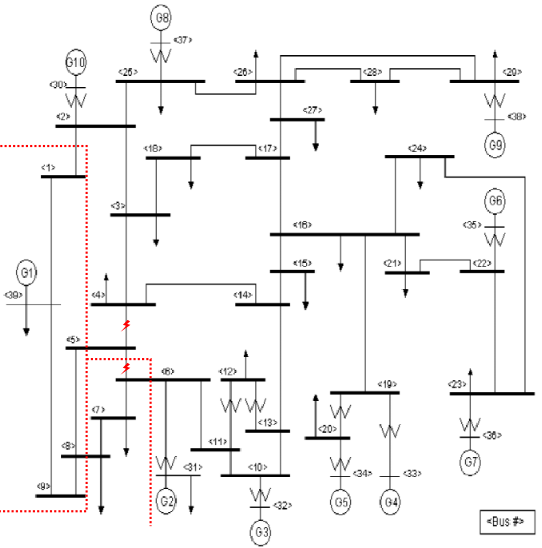
\includegraphics[width=0.475\linewidth]{Figs/IEEE39_slow_split.pdf}
        \label{subfig:split_slow}
    } \hfill
    \subfloat[System split following the (actual) fast sequence]{%
        \includegraphics[width=0.475\linewidth]{Figs/IEEE39_fast_split.pdf}
        \label{subfig:split_fast}
    }
    \caption{Comparison of the consequences of the N-2 contingency of lines 5-6 and 6-7 in the slow and fast sequences}
    \label{fig:IEEE_split}
\end{figure}
}

% 6.15694 | 1-_2-1_AC_side2_DistanceSlow | Distance protection trip zone 2
% 6.22741 | 1-39-1_AC_side1_DistanceSlow | Distance protection trip zone 2
% 6.25709 | 5-_8-1_AC_side1_DistanceSlow | Distance protection trip zone 3
% 6.34501 | 8-_9-1_AC_side1_DistanceSlow | Distance protection trip zone 2
%
% 6.02905	13-14side1_Distance	Distance protection trip zone 3
% 6.05505 | 1-_2-1_AC_side2_DistanceFast | Distance protection trip zone 2
% 6.13181 | 5-_8-1_AC_side1_DistanceFast | Distance protection trip zone 3
% 6.134 | 1-39-1_AC_side1_DistanceFast | Distance protection trip zone 2
% 6.15187 | 4-14-1_AC_side2_DistanceFast | Distance protection trip zone 3
% 6.18391 | 8-_9-1_AC_side1_DistanceFast | Distance protection trip zone 2
%
% 6.02905	13-14side1_Distance	Distance protection trip zone 3
% 6.05505	1-2side2_Distance	Distance protection trip zone 2
% 6.13181	5-8side1_Distance	Distance protection trip zone 3
% 6.18407	8-9side1_Distance	Distance protection trip zone 2
% 8.27884	GEN___38_SM_Speed Under-speed protection trip
% 8.31923	GEN___37_SM_Speed	Under-speed protection trip
% 8.32712	GEN___30_SM_Speed	Under-speed protection trip
% 8.35866	GEN___33_SM_Speed	Under-speed protection trip
% 8.36521	GEN___35_SM_Speed	Under-speed protection trip
% 9.43916	23-24side1_Distance	Distance protection trip zone 2
% 9.55622	26-27side2_Distance	Distance protection trip zone 3
% 9.60304	16-17side1_Distance	Distance protection trip zone 3
% 9.81107	16-21side2_Distance	Distance protection trip zone 3
% 9.81712	GEN___33_SM_UVA	Under-voltage generator trip
% 9.84866	GEN___34_SM_UVA	Under-voltage generator trip

It can be noted that looking at the sequences of protection operations allows the indicator to perform significantly better than an indicator that would only consider the consequences of cascades. For example, Table~\ref{tab:indicator-consequence-based} shows the performance of an indicator that is true if the slower and faster sequences lead to different amount of load shedding%\footnote{Note that to estimate the load shedding, both sequences need to be simulated separately.}
. Such indicator indeed shows poor performance and misses between 20\% and 44\% (depending on the load model) of the sensitive contingencies.


\subsubsection{Causes of false negatives and false positives}
\label{sec:causesOfInaccuracy}

% 1s-restorative case, 3 FN
% _BUS___26-BUS___27-1_AC_end1-CB_end1-_BUS___26-BUS___29-1_AC
% Faster disconnection of GEN___38_SM_Speed that lost synchronism leads to less UFLS
% _BUS____2-BUS___25-1_AC_end2-CB_end2-_BUS___25-BUS___26-1_AC
% _BUS___26-BUS___29-1_AC_end2-CB_end1-_BUS___26-BUS___27-1_AC
% Same

% 5s, 1 FN
% _BUS___26-BUS___29-1_AC_end1-CB_end1-_BUS___26-BUS___27-1_AC
% Same

Table~\ref{tab:indicator} shows that the indicator misses 4 sensitive contingencies (3 false negatives in the 1s-restorative-load case, and 1 in the 5s-restorative one). In all those 4 cases, the difference between the slow and the (actual) fast sequences is that, in the fast sequence, generator 9 (bus 38) is disconnected faster by its protections after losing synchronism. This faster disconnection helps with frequency stability and leads to the activation of one less UFLS step. In the fast sequence estimated from the simulation of the slow one, this impact on the frequency behaviour is not caught, which leads to the false negatives. Using two simulations (one for the slower sequence and one for the faster sequence) would thus have lead to a null false negative rate (at the cost of an increase in computation time).

Table~\ref{tab:indicator} also shows that the indicator has a few false positives. It should however be noticed that false positives have a smaller impact that false negatives. Indeed, false negatives hide sensitive contingencies and lead to an inaccurate evaluation of their consequences (estimation from a single simulation while multiple MC simulations would be needed). However, false positives only cause unnecessary MC simulations which only affects computation time.

There are two causes for the occurrence of false positives. The first is that, in some cases, changing the order of protection operations does not impact the global evolution of the cascade. A typical example of this is when two distance protections operate to split the system in different points following an out-of-step condition. In this case, changing the order of protection operations will sometimes impact how the system splits and sometimes not.

The second cause is due to contingencies in which the operation of an additional protection system does not impact the consequences (in terms of load shedding). Most often, the protection system has no impact because it operates in an island that will collapse regardless of whether the protection system operates. % Both causes are each responsible for around 50\% of the false positives. % Also, one case where the ``new" protection that operates is Z3 instead of Z2 of the same protection -> actually not impact (most likely that Z2 will trip first anyway and that Z3 thus cannot trip after)


\section{Conclusion}
\label{sec:protection_conclusion}

Protection systems play a key role in maintaining highly-reliable power systems. However, they can sometimes misoperate, and they also impact (in positive and negative ways) the evolution of cascading outages. It is thus critical to model them adequately when performing probabilistic security assessments.

For this, it is important to first acknowledge the fact that protection systems can sometimes fail to clear faults in the normal way (i.e. by quickly disconnecting the faulted element), transforming mild N-1 contingencies into more severe N-k contingencies. This is because protection systems cannot be made 100\% dependable nor 100\% selective. Lack of dependability is mainly caused by the failure of individual protection elements (relays, breakers) and can be adequately modelled using standard reliability evaluation techniques such as fault trees and event trees. This is discussed in great details in~\cite{GridPSA, Haarla}.

Lack of selectivity has more diverse causes, including design errors, incorrect settings, and as-left personnel errors~\cite{ProtectionMisoperationsBian2012} that are significantly harder to model. Most of the literature on the topic is rather old and is concerned with failure modes of legacy electromechanical relays that are no longer used. Unfortunately, due to lack of time, this issue was not investigated further in this thesis and is left for future work. But, statistics on the rate and causes of unselective protection behaviour at extra-high voltages (the ones most critical for security-related issues) would greatly help in evaluating the importance of unselective trips and to model them.

Beyond clearing the initial faults, protection systems also play a key role in how cascading outages propagate. As for fault clearing, lack of dependability or of selectivity can impact cascading outage evolution\footnote{Although, as will be shown in chapter~\ref{ch:DPSA}, the impact lack of dependability is relatively limited, except for SIPSs.}. However, even with perfectly reliable protection systems, it is difficult to predict how protection systems will impact the evolution of cascading outages. Indeed, during cascading outages, many protection systems might operate or be close to operate in a short window of time. Therefore, the propagation of cascading outages (and thus their final consequences) can be very sensitive to modelling uncertainties. In the literature, this has been studied using advanced MC techniques~\cite{SequencesRelaySobol, PierreIEEEtran}, however MC simulations are computationally expensive which is problematic for the probabilistic security assessment of large systems that require to simulate many possible cascading outages. To alleviate this issue, this thesis proposes a simple indicator to predict which cascading outages are actually sensitive to protection-related uncertainties, so that MC simulations can be focused on these cases.

In conclusion, this chapter has discussed how to model N-k contingencies caused by protection misoperations and how to model the impact of protection systems on the evolution of cascading outages. The next step is thus to integrate this information into a comprehensive probabilistic security assessment framework. This is the objective of chapter~\ref{ch:DPSA}.

\chapter{Model of distribution grids}
\label{ch:distrib}
\minitoc

It has long been acknowledged that load models play have a critical influence on the results of dynamic simulations, especially on voltage stability~\cite{kundur}. Most utilities however use relatively (e.g. compared to generators) simple load models due to the difficulty to gather data on the loads connected to the distribution grid and their variable nature\footnote{Both the total amount of load and shares of different types of loads (heaters, motors, lamps, etc.) vary with the time of day and the season.}. The most commonly used model is the ZIP load model (aggregation of a constant impedance, a constant current and a constant power load) and its derivatives~\cite{IndustryLoadModel}.

The massive installation of distributed renewable energy sources (mostly wind and solar) in distribution grids challenges those load models. In particular interest in this thesis is the tendency of distributed generators to disconnect during wide-area disturbances. These disconnection had a high impact in historical blackouts. For example, the frequency collapse of Italy in 2003 was partly caused by the unexpected disconnection of 3400~MW of distributed generators while the frequency was still above 49~Hz~\cite[p115]{Italy2003}. On the other hand, there are perspectives regarding the provision of ancillary services by distributed generators. Better modelling of those so-called active distribution networks (ADNs) is thus needed.

One way to accurately model the interactions between the transmission and distribution sides of a grid is to perform simulations on complete a transmission and distribution network as in~\cite{FullTDexample}\footnote{To limit the size of the studied system, it is of course necessary to only consider the medium voltage level of the distribution grids, not the low voltage level.}. However, this approach cannot be used in this thesis due to the high computational power requirements of probabilistic dynamic security assessment. Outside the scope of this thesis, this approach also has issues of confidentiality and data handling.

% Co-simulation of T\&D (gridlabd?)

Reduced-order load models are thus necessary. Section~\ref{sec:dynLoadModel} thus reviews load models used in the literature%, and section~\ref{sec:dynLoadModelParam} discussed how to estimate the parameters of these load models.
and section~\ref{sec:loadPerspectives} discusses perspectives.

\section{Passive load models}
\label{sec:dynLoadModel}

Load models have seen renewed interest in the past decade due post-mortem reproduction of some blackouts being impossible with simple ZIP models~\cite[p11-12]{CIGREloadModels}. It was shown necessary to include at least a simple model of induction machines as in Fig.~\ref{fig:motorLoad}. The model of the induction machine can be either static (i.e. only include algebraic equations, so consider the slip \(s\) to be constant) or dynamic (i.e. differential-algebraic equations, so the slip varies with time as a function of the balance between the electromagnetic and load torques). More complex load models such as the WECC composite load model (CLM) have also been developed. The CLM is shown in Fig.~\ref{fig:WECC-CLM}. It consists in an on-load tap changer (OLTC), and equivalent feeder impedance, four different types of dynamic induction motor models, and electronic and a static (i.e. ZIP) load. It is being implemented in several time-domain simulators~\cite{NERCloadModelTF}. Various models whose complexity is between the ZIP and CLM models have also been developed and are reviewed by the CIGRE~\cite{CIGREloadModels} and NERC~\cite{NERCloadModelTF} task forces on load modelling.

\begin{figure}[t]
    \centering
    \includegraphics[width=0.6\linewidth]{Figs/MotorLoad.png}
    \caption{Constant impedance load in parallel with an induction motor~\cite{CIGREloadModels}}
    \label{fig:motorLoad}
\end{figure}

\begin{figure}[t]
    \centering
    \includegraphics[width=0.5\linewidth]{Figs/WECC-composite-load-model.png}
    \caption{WECC composite load model~\cite{NERCloadModelTF}}
    \label{fig:WECC-CLM}
\end{figure}

The models presented above however do not consider distributed energy sources. The simplest solution to this is to add one (or several) generic model(s) of renewable sources to the load model. However, estimating the parameters that give the most accurate representation of the system might be difficult, especially since TSOs have little experience with ADNs compared to ZIP and motor load models. So, four main types of methods were developed in the literature to build ADNs models. They are listed below~\cite{ADNreview2013}.

\begin{itemize}
    \item Linear-based approaches: in these methods, the model of the full distribution network is first linearised. Then, different approaches (e.g. Hankel-norm approximation, modal approach, Krylov methods, etc.) allow to reduce the order of the linearised system. A theoretical bound on the error made by using the reduced-order model can be derived depending on the method used. These methods are however accurate only around a given operating point and are thus not appropriate to study large disturbances. These methods were originally developed to make reduced-order equivalents of neighbouring transmission systems. Indeed, TSOs mostly study the impact of disturbances originating in their own system. For moderately large disturbances, neighbouring TSOs are weakly affected, so a linearisation-based approach makes sense. Distribution systems however are much more dependant on their associated transmission system.
    \item Coherency-based approaches: synchronous generators that tend to swing together are grouped into an equivalent machine. The network around those machines is then also reduced. Like linear-based approaches, these methods were developed to model neighbour transmission systems. They are often not applicable to distribution systems as synchronous generators are rarely used there.
    \item Black-box approaches: in these methods, the model of a distribution system is an artificial neural network (ANN) that is trained to match the behaviour of the actual distribution system. These methods are quite popular since they do not require any information on the structure and components of the distribution grid. ANNs are thus most often matched to measurements of the behaviour of the distribution grid (often PMU measurements made at the point of common coupling (PCC) between the transmission and distribution grids). It is also possible to train ANNs from simulations of the distribution grid, but grey-box approaches (described below) are often preferred when one has enough information on the distribution grid to simulate it. The main limitation of measurement-based approaches (and by extension black-box approaches) is that large disturbances are rare. It is possible to intentionally introduce disturbances to generate more data but those disturbances are usually kept small for obvious reasons (usually tap changes or capacitor switching). Training ANNs for those disturbances is thus often impossible.
    \item Grey-box approaches: grey-box approaches are similar to black-box approaches except that the model used is a physical model instead of an ANN. The model usually has at most a few buses and should have a similar structure than the real grid\footnote{Taking the example shown in Fig.~\ref{fig:greyBox}, if switches a and b are closed, and switch c is open, they grey-box model becomes two feeders in parallel. One feeder could represent a classical distribution system. The second, a large distribution-connected plant (with stricter connection requirements).}. The advantage is thus that results are more comprehensive, but it is necessary to known  the structure of the distribution grid. An example of grey-box model is shown in Fig.~\ref{fig:greyBox}. Like black-box approaches, the parameters of the model are fitted to match the behaviour of the full model (e.g. in the least square sense). As it is not feasible to write the analytical formulation of the objective function (i.e. difference between behaviour of the grey-box and the real system), derivative-free optimisation methods (e.g. genetic algorithms, particle swarm optimisation) have to be used. The behaviour of the real system for a given operating point and disturbance can be obtained either from measurements or from simulations. As previously explained, only the simulation-based approach is appropriate when studying large disturbances\footnote{When available, measurements should still be used to validate the equivalent and/or the full distribution model.}.
\end{itemize}

\begin{figure}
    \centering
    \includegraphics[width=0.6\linewidth]{Figs/GreyBoxEquivalent.pdf}
    \caption{Possible grey-box equivalent topologies. Multiple topologies can be created from this scheme by changing the status of the switches~\cite{ChaspierreThesis}. IBG = Inverter-based generation}
    \label{fig:greyBox}
\end{figure}


As discussed above, only (simulation-based) grey-box approaches are suitable to study large disturbances. This is thus the type of approach chosen in this thesis. Most recent development on grey-box approaches have been made in the thesis of Gilles Chaspierre~\cite{ChaspierreThesis, ChaspierrePaper}. His approach is thus used as a reference in this thesis. He also proposed a methodology to share the grey-box development between the TSO and DSOs to avoid confidentiality issues, and he discussed how to efficiently update the equivalent with varying operating conditions. Interestingly, he also proposed a control algorithm for a battery storage to be installed at the PCC to compensate for errors between the grey-box and the real system. Those elements are however not discussed further here.


\section{Perspectives}
\label{sec:loadPerspectives}

The results in~\cite{ChaspierreThesis} were very satisfactory, so relatively little improvements can be performed\footnote{A more detailed discussion of potential improvement is done in section 7.2 of~\cite{ChaspierreThesis}.}. Two main paths can be considered in this thesis. The first is the validation of grey-box models in large-scale studies. Indeed, in the literature, ADN equivalents (including grey-boxes, black-boxes, etc.) are validated in studies were only one distribution system is replaced by an equivalent (the others are simply considered to always behave as simple load models). In this thesis, studies will be performed by replacing all loads by equivalents. Additionally, as I study cascading outages, the models will be further challenged.

Another path to consider is the handling of model uncertainties. In~\cite{ChaspierreThesis}, the complete model of the distribution system is simulated with random sets of parameters (e.g. parameters of the control loops of distributed generation, share of renewables, etc.) to account for uncertainties. From these simulations, one deduces the average (i.e. statistical expected) behaviour of the system as well its standard deviation. This is illustrated in the example in Fig.~\ref{fig:greyBoxUncertainty}. The grey-box is then fitting to the average, and the objective function is a least square error weighted by the standard deviation for each point in time. In the rest of the literature, uncertainties are not considered (except measurement errors in measurement-based approaches). In this thesis, I might try to determine if using a single equivalent is appropriate, or if using multiple equivalents associated with different realisations of the uncertainties is necessary. Also, methods to propagate the uncertainties from the full model to the equivalent might be considered. % Correlation between uncertainties of different distribution grids (e.g. LVRT of a given manufacturer)

% "Probabilistic load model": transfer the uncertainty in parameters of full model into the reduced one. And/or sensitivity studies.

\begin{figure}
    \centering
    \includegraphics[width=0.6\linewidth]{Figs/GreyBoxUncertainty.png}
    \caption{Average \(\mu_P\) and standard deviation \(\sigma_P\) of the active power consumption of a distribution grid following a disturbance at \(t=\)0.3~s~\cite[p58]{ChaspierreThesis}}
    \label{fig:greyBoxUncertainty}
\end{figure}


Finally, as this thesis is made in the framework of the CYPRESS project (presented in appendix~\ref{ch:CYPRESS}), the possibility to include cyber elements in the equivalents will be studied.

\TODO{Fig of equivalent with average parameters vs. correct ones (in draft of ISGT paper), not fully accurate but already way better than simple load model}

\TODO{(fig 4 of CIGRE paper shows it would be best to cluster, but does not work for multiple disturbances)}


% Assume already have the appropriate load model for each moment of year -> do not include in computing time for DPSA
\chapter{Probabilistic dynamic security assessment}
\label{ch:DPSA}
\minitoc

\TODO{Load blinders added compared to chapter~\ref{ch:protections}}

Need more data than deterministic. It should be noted that, even if using more complex models, the exact value of the risk (in MWh/y or €/y) is of low significance. What is important is to be able to compare the risk associated with different scenarios and to be able to identify actions that most effectively reduce the risk.

PDSA will provide useful information even with garbage data, but better data gives better results \url{https://xkcd.com/2295/} ('Garbage In, Garbage Out' should not be taken to imply any sort of conservation law limiting the amount of garbage produced.)

Limit analysis to short-term stability for sake of simplicity, but could be applied to long-term too (or both, Eurostag, Dynawo)

\TODO{ML figure: coverage, importance, historical}

\TODO{Show more the ximple windows than in paper (e.g. likelyhood of a contingency having consequcens, etc.)}

\TODO{Mention missing trips (other than fault clearing)}

\TODO{Use the DPSA acronym. Potentially distinguish between DPSA and probabilistic DSA}

\TODO{Explain the choice of considered failure modes: EHV faults most likely to causes wide-area issues, EHV protected by diff+distance (in Elia) and talks for double diff, diff is a very good protection, cannot really be misconfigured and self-testing of relays (incl. more advanced stuff like Russian paper in CIGRE 2022 proceedings)}

\TODO{(D)PSA is more of a process than a methodology, refine the models/data by iteration}

\TODO{Curse of dimensionality / peel, example with hypersphere}

\TODO{Bien situer le contexte (vision planing mais opérationel envisable avec modifications), ce qui existe déjà, etc.}

Limit analysis to short-term stability for sake of simplicity, but could be applied to long-term too (or both, Eurostag, Dynawo), same for ch 6

\TODO{Protection indicator helps a bit with coverage, although don't know how much}

The objective of a probabilistic security assessment are to list the possible accident scenarios that can lead to unwanted consequences, to estimate the probability of these scenarios, and to estimate their consequences. Such assessment can be decomposed into two parts: (i) listing (or sampling) the possible pre-contingency states, and (ii) determining the possible post-contingency evolutions. As highlighted in the literature review (section~\ref{sec:probabilisticSecurity}), the second part is actually the hardest.

In a deterministic approach, only one post-contingency evolution is considered, because one assumes that all transmission equipment and protection systems operate as expected. The evolution is computed by simulation. Often, the protection systems are not explicitly modelled in the simulation. Their effect (e.g. fault clearing by opening a line) is predicted in advance and included in the simulator as part of the contingency. In a probabilistic approach, possible misoperations are considered which leads to multiple possible system evolutions. One way to handle those multiple possible evolutions is to use event trees as done in~\cite{Haarla, GridPSA}. Event trees are presented in section~\ref{sec:DynMethods} and in Figure~\ref{fig:eventTree}. In the approach proposed in~\cite{Haarla, GridPSA}, event trees are built prior running simulations. So, only events that can easily be predicted without simulations can be included\footnote{For example, if the initiating event is a line fault, the events that can easily be predicted are the triggering of the protections of this line, and their backup protections.}. Another limitation of event trees is that event are placed in a so-called event axis instead of a time axis. So, it is assumed that the timing of events does not influence the evolution of the system.

In theory, a skilled analyst can alleviate the above limitations. He can use his expertise and/or simulation results to identify events that can occur during the system evolution. Also, if the order and/or timing of events is of importance, he can add additional events to consider them (e.g. split ``event A occurs" in ``events A occurs before \(t=\)~5~s" and ``event A occurs after \(t=\)~5~s). It can however be difficult to compute the probabilities associated with those events. Also, the analyst should try to only consider the most critical scenarios to avoid an explosion of the size of the tree. So, in practice, this requires a lot of effort from the analyst. So-called dynamic event trees (DETs) have thus been developed with the objective to move most of the burden of proof of correctness from the analyst to the methodology. DETs are introduced in section~\ref{sec:dynamicReliability}.

It should however first be noted while the above observations have mostly been made in the nuclear sector (wherefrom event trees originated)~\cite{LabeauTowards}, they are even more relevant for power systems. There is two main reasons for this. First, there are significantly more initiating events to consider. Indeed, one should consider at least hundreds of possible (e.g. line) faults or even more depending on the size of the considered system (and the voltage level(s) considered). Also, for a given fault, multiple event trees should be built as the evolution of the system depends on the initial operating conditions. Second, a large number of events can occur after a disturbance, especially during fast cascading outages. Predicting those events as well as determining the importance of the timing and order of events might prove particularly complex.

Section~\ref{sec:dynamicReliability} introduces DETs and reviews the literature on the subject. Section~\ref{sec:proposedMethodology} discusses the proposed methodology. Section~\ref{sec:DataRequirementsForDSA} discusses the data requirements for dynamic probabilistic security assessment, and section~\ref{sec:testCases} presents the test cases used.


\section{Dynamic reliability methods}
\label{sec:dynamicReliability}

\textbf{Note:} In the final thesis, this section will introduce more rigorously DETs and the different techniques that can be used to solve them. Also, ``dynamic reliability" techniques (that include DETs) will be reviewed. In this report, only MCDET, the specific DET solving technique used in this work, is presented.

A DET follows the (time-dependant) evolution of the system after a given initiating event. This tree branches each time the system can transition to different states. For example, if the initiating event is a line fault, the DET will branch at the times when each of the circuit breakers (CBs) open. In that case, each branch is associated with a possible state of the CBs (i.e. both open, both closed or one open and one closed) and follows the evolution of the system in that given state. Additionally, because the operating time of the circuit breakers is not known with an infinite precision, branchings are made at each point in time were the breakers are likely to operate. If CB opening times are assumed to follow some continuous probabilistic distribution, there is theoretically an infinity of possible branching points to consider. Techniques are thus needed to solve them numerically.

It should be noted that contrarily to ``static" event trees, branching points are not defined explicitly but via branching rules. For example, if the line is protected by distance protection scheme, the relays and CBs should be included in the model. Then, during the system evolution, when the apparent impedance seen by a relay goes below a (potentially uncertain) threshold, the relay send a tripping signal to the CB that either opens (after an uncertain amount of time) or fails to open. Branches are automatically created to follow the possible system evolutions (e.g. CB fail to open, CB opens 60~ms after receiving the signal, CB opens 80~ms after receiving the signal, etc.).

One of the available techniques is MCDET. MCDET is a concatenation of MC (Monte Carlo) and DDET (discrete DET). In MCDET, continuous uncertainties (e.g. threshold values, CB opening delays) are handled by MC and discrete uncertainties (e.g. CB fails to open) are handled by DDETs. DDETs are based upon the restriction of the possible branching points to discrete points in time. In other words, the system evolution after a disturbance is simulated, and at each time step branchings are created following aforementioned branching rules. The drawback of DDETs is the combinatorial explosion of the number of branches (that grows as the average number of branches created at each step to the power of the number of steps). To manage this explosion, it is necessary to introduce cutoffs (e.g. do not follow branches that have a probability lower than a threshold) and to increase the size of the time steps. It is however difficult to estimate how the size of the time steps and the cutoff thresholds affect the accuracy of the DET solving method. So, it is difficult to make a good compromise between accuracy and computation time.

In MCDET, a DDET is built for each (MC) sample of the continuous uncertainties. As only discrete uncertainties have to be handled by the DDETs, they can potentially be built completely (i.e. with no cutoffs and a very small time step). In this case, the accuracy of the DET solving technique depends only on the MC part. This is convenient as MC accuracy can be estimated easily with statistical methods.


\section{Proposed methodology}
\label{sec:proposedMethodology}

As discussed in the previous section, the security assessment method used in this thesis is based on MCDET. An additional element has however to be added to the methodology to properly model the pre-disturbance state of the grid. Indeed, given a particular realisation of generator and transmission asset availabilities and load, system operators will try to dispatch power plants to minimise total costs while maintaining acceptable operating conditions (e.g. no overloads, acceptable voltages, etc.). The optimisation problem associated is called an optimal power flow (OPF). When potential (usually N-1) contingencies are considered, this is referred to as a security constrained (SC) OPF.

The methodology can thus be summarised as follow. First, generate a sample of the pre-contingency state (i.e. availability of assets, renewable production, etc.) and consolidate it by running a (SC)OPF program. Then, sample the remaining continuous uncertainties. Build a DDET to handle the discrete uncertainties. Repeat the above procedure until statistical convergence.

\TODO{Simplified model of a few steps of slow cascade?}
% \TODO{Mention forecasting errors for the SCOPF? (not considered in the thesis)}
\TODO{(Foot)note: sampling protection threshold before simulation implies ``tabou" region~\cite{Faghihi}.}


\section{Data requirements for dynamic probabilistic security assessment}
\label{sec:DataRequirementsForDSA}

Dynamic probabilistic security assessment requires a large amount of input data. The following paragraphs thus discuss the data needed to model the pre-disturbance state, the disturbances themselves, and the post-disturbance evolution.

\subsection{Pre-disturbance state}

The data required to model the pre-disturbance state of the grid is quite similar to the one used in deterministic dynamic security assessment (that is discussed e.g. in~\cite{EurostagHPC}). These data consist mainly of generation and load forecasts for the considered period. Planned maintenances are also often included. In a probabilistic assessment, the only additions could be unplanned maintenances and forecast errors. These are not considered in this thesis. Finally, the (SC)OPF also requires some data: running costs of generators (or at least a merit order) and static (current) limits.

\subsection{Disturbances}

In a probabilistic assessment, it is of course necessary to estimate the frequency of occurrence of disturbances. This requires historical statistics of past disturbances.

\subsection{Post-disturbance evolution}

Modelling the post-disturbance evolution of a system in a probabilistic assessment is generally more complex than in a deterministic one. This is because, in a probabilistic analysis, the system has to be simulated further away from normal operation (e.g. during cascading outages). For this, one should generally model the generators (including governors and voltage regulators), loads, transformers, etc. with the best (RMS) models available. If the accuracy of a model is deemed insufficient (e.g. difficulty to reproduce past disturbances, high sensitivity to input data, etc.), then better models have to be developed and/or better data have to be collected.

Additionally, since the system is simulated in degraded states, protections have to be modelled explicitly\footnote{At least, the protections that are discussed in chapter~\ref{ch:protections}.}. This requires to know what protections are installed in the system and what are their settings. Finally, to compute the frequency of scenarios, it is necessary to have an estimate of the probability of failure of protection systems. It is best to also have probability density functions (pdfs) of the protections thresholds\footnote{In order to model measurement and setting errors. The second point is particularly challenging.} and operating times. Pdfs of all aforementioned parameters can also be used to refine the analysis and perform sensitivity studies.

\TODO{2-3 mots sur ce qu'Eurostag appèle le modèle electromec étendu (p117)}

\section{Test cases}
\label{sec:testCases}

The method proposed in this thesis will be applied on a variety of test cases. This report present two of them: the Roy Billinton test system (RBTS) and the three-area reliability test system (RTS). They are shown in Figure~\ref{fig:rbts-ch6} and~\ref{fig:rts} respectively. These systems were chosen because they include part of the necessary data (static data, load and generation profiles\footnote{The grid modernization laboratory consortium (GMLC) developed an updated version of the RTS. This version has a significant installed capacity of renewable generation. It also mapped the system to a geographical area such that meteorological data can be used to generate coherent generation forecasts.}, economic data). Missing data include dynamic data (i.e. generator models) and protection data (types of protection installed, settings and reliability data). Another criterion in the choice of these systems is their size. The RBTS is a small (6-bus) system that can be used in simple case studies and for debugging. The RTS is a medium (73-bus) system that is large enough to represent cascading mechanisms found in larger grids, yet not to large which eases the interpretation of results, data handling and computational issues\footnote{Finally, those systems were developed for research on reliability. Contrarily to other systems, parallel lines and parallel generators are not replaced with equivalent elements. This allows to more easily perform N-1 security analysis (double line failures are not accidentally considered as N-1 contingencies) and fill the missing data (generators have more realistic sizes, so typical parameters are easier to find).}.

\begin{figure}
    \centering
    \includegraphics[width=0.6\linewidth]{Figs/RBTS.png}
    \caption{Roy Billinton test system. Adapted from~\cite{rbts}}
    \label{fig:rbts-ch6}
\end{figure}

\begin{figure}
    \centering
    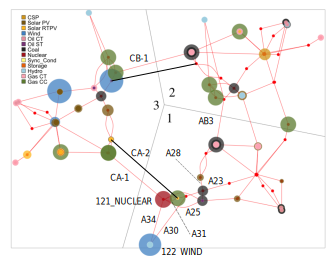
\includegraphics[width=0.8\linewidth]{Figs/RTS.jpg}
    \caption{Reliability test system~\cite{VOLL}}
    \label{fig:rts}
\end{figure}

The following dynamic data have been added to those systems. Synchronous generators are represented with a seventh order model. For most generators, the excitation system is represented by an IEEET1 model, and the governor is represented with BPA GG (also known as WSCC type G) model as in~\cite{excitationAndGovernorModels}. A different model is however used for hydro units as they have a fundamentally different behaviour than other types of units. The model used is an GOVHYDRO1 model. Most parameters are taken from annex D of~\cite{vittalBook}. This annex contains typical data for different types of machines (hydro, nuclear, coal, gas) and a wide range of rated powers (5~MW to 1.3~GW). So, for each generators of the test systems, parameters were taken from a machine in~\cite{vittalBook} that has the same type and that has the closest rated power. For hydro units, those parameters are completed with the ones in~\cite{hydroGov}. Models of wind and solar plants still have to be defined. However, WECC models or the generic inverted-connected generation model proposed in~\cite{ChaspierreThesis} will probably be used. Protection models are discussed in chapter~\ref{ch:protections}.

\TODO{Check this 7th order stuff if I have the time, or say ``four winding model" model (one field winding, one d-axis damper winding and two q-axis damper windings) according to Dynawo terminology.}

'Subsequent analysis is required to understand and mitigate high
numbers of unsuccessful simulations'\cite{EurostagHPC}


\TODO{robustness analysis even if out of scope of ``purely-probabilistic" assessment. E.g. redo analysis with all loads increases by 10\% (but with lower statistical accuracy requirements)}

% \cite{TestSystemHenneaux} % for RTS modifications to be N-1 secure

% \subsection{RBTS}
% \label{sec:RBTS}

% will be modernised by decreasing coal capacity (and replace by gas) and add RES in distrib.

% \subsection{GMLC-RTS}
\chapter{Conclusions and future work}
\label{ch:perspectives}

Society has grown to expect electricity to be available at any time and any interruption of service can thus have massive consequences both from an economic perspective (production downtime, equipment damage) and from a social perspective (injuries due to the lack of electricity, civil disorders). To meet those reliability expectations, power systems have often been designed around the N-1 security criterion that states the system should always be able to withstand the loss of any single element. However, past disturbances have shown that, although rarer, N-2 and higher order contingencies can occur and lead to cascading outages and widespread blackouts. On the other hand, the increasing share of intermittent energy sources indicate and economic pressure are pushing for TSOs to relax the N-1 criterion for system conditions that are deemed as unlikely or infrequent. There is thus an increasing willingness of TSOs to complement the deterministic N-1 criterion with probabilistic methods that can more adequately estimate the risk of blackouts and balance it with the cost of avoiding those blackouts. In this context, the objective of this thesis was to develop a probabilistic methodology to identify the scenarios most likely to lead to blackouts and to estimate their frequency and consequences. More specifically, this thesis focused on cascading outages initiated by short-term stability issues.

\section{Main Contributions}

Probabilistic methodologies require more advanced models than deterministic ones. Most importantly, protection systems play a key role in the initiation and propagation of cascading outages and have thus been studied in chapter~\ref{ch:protections}. Indeed, failure of protection systems to isolate faults can transform mild N-1 contingencies into more severe N-k ones and initiating a cascading outage. To model these failures, standard reliability techniques such as failure mode and effect analysis and event trees can be used. The application of these techniques to power systems are extensively described in~\cite{GridPSA}, and this thesis reuse this work to define contingency list to be considered in a probabilistic dynamic security assessment and to estimate the frequency of occurrence of such contingencies.

Conversely, the impact of protection systems during cascading outages in more difficult to model. Indeed, during cascading outages, and especially fast cascading outages, many protection systems might operate in a short period of time. This implies that the evolution of cascading outages can be very sensitive to the timing of protection system operations. In the literature, this sensitivity has been handled (when not disregarded) with multiple Monte Carlo methods. However, these methods are too computationally expensive to be used in systematic analysis that consider many possible contingencies in large systems. This thesis has thus proposed an indicator to predict which scenarios lead to cascading outages that are sensitive to the timing of protection systems operations and which are not, so that Monte Carlo simulations can be focused on the former.

Another class of models that require more consideration in probabilistic security assessments than deterministic ones is the models of distribution grids that were studied in chapter~\ref{ch:distrib}. Indeed, distributed energy sources tend to disconnected themselves during severe disturbances further degrading the state of the system. Similarly, motors are more likely to stall in those conditions leading to cascading effects. However, due to the low observability of distribution grids and the sheer number of elements connected to them, there are many uncertainties in the models of distribution grids. To handle those uncertainties, this thesis has proposed to build two dynamic equivalents per distribution grid model to bound the likely behaviour of distribution grids. It was then shown that performing transmission-level studies with those two equivalents gave similar confidence intervals as if full probabilistic transmission and distribution simulations were performed but in a much more practical manner. These equivalents have be shown to be adequate to model cascading outages and real power systems.

With those models built, chapter~\ref{ch:DPSA} has been able to develop a probabilistic dynamic security assessment methodology. This type of methodology generally consists in applying many contingencies into randomly sampled states of the grid, evaluating the consequences that would have such contingencies, and continuing until some statistical accuracy criterion is satisfied. In the literature, stopping criteria are often based on the standard error of the total risk, but in this thesis, it was argued that it is more useful to have an accurate estimate of the risk of individual contingencies. Indeed, most security-enhancing actions focus on solving local issues and thus affect the security of a limited number of contingencies. Then, a rigorous statistical accuracy indicator had to be developed to guarantee that no important unsecure regions are missed when sampling operating conditions. Based on this indicator, it was shown that when trying to have an accurate estimation of the risk of individual contingencies (as opposed to the total risk), the most effective sampling approach is generally a crude MC sampling, i.e. sampling of contingencies and operating conditions proportional to their probability of occurrence. To alleviate the computational burden of such crude MC approach, screening techniques and an implementation in a high-performance computing environment have been developed. The method has been applied to a 73-bus system and a scalability study has shown that the proposed method could be applied to large power grids with high but manageable computation burden.

The application of the methodology to a test system has also shown that a limited number of critical contingencies generally contribute to a large share of the total risk. In the considered test system, the 10 most critical delayed-clearing N-1 contingencies and N-2 contingencies (out of 708 considered contingencies) contributed to 44\% of the total risk. This indicates that complementing the N-1 criterion by securing a limited number of more severe contingencies could significantly reduce the risk and be cost-effective.

One drawback of probabilistic methods is that they require to perform many simulations which makes their results more difficult to interpret compared to deterministic methodologies. This drawback is partially alleviated by the fact that the analysts can focus on a small set of critical contingencies. In the considered test systems, 150,000 simulations were performed, but ``only'' a few hundreds were run for a given contingency. Moreover, it has been shown that by looking at which protection systems operate at the start of the simulated cascades, it is often possible to group those simulations in only a few different cascades sequences and to identify the root causes of insecurity. To help with the interpretation of the results, simple machine learning techniques have also been proposed to have an ``automatic'' identification of the root causes of the insecurity by identifying the boundary between secure and unsecure operating conditions for a given contingency. These identified security boundaries could also be used as operational rules to increase the security of the system at the cost of increased operating costs. One advantage of probabilistic methods is that these increased operating costs can be directly compared to the estimated reduction in unreliability costs (i.e. costs of occasionally having cascading outages and blackouts).

\section{Discussion}

The objective of this thesis was to develop a probabilistic dynamic security assessment methodology to cope with the limitations of deterministic methodologies. However, probabilistic methods do have drawbacks, some of which have not been properly acknowledged in the core of the thesis and are thus discussed here. Most importantly, probabilistic methodologies require significantly more data than deterministic ones, particularly reliability data: (weather-dependent) frequency of occurrence of faults, analysis of the failure modes of protection systems and estimation of their likelihood, etc. that require significant data collection campaigns over many years. However, without minimising the need for those campaigns, it should be noted that probabilistic security assessments can provide valuable insights even with incomplete data. Actually, in other fields (nuclear, aviation, oil and gas, etc.), it is common to perform probabilistic \emph{safety} assessments (PSA) with engineer best estimates for failure rates and other reliability data, at least in a first stage. Critical components can then be identified, and this, with sensitivity studies on the uncertain parameters, can help focussing data collection on the most important parameters.

Actually, in the nuclear sector, it sometimes said that the numerical value of the total risk estimated from a PSA is of little importance (despite being a regulatory target), and that what actually is the identification of critical components and the provision of recommendations on how to effectively reduce the risk. This statement might be more or less valid depending on whether one tries to minimise the risk following the as low as reasonably achievable (ALARA) approach (or as low as achievable with a fixed budget), or following a cost optimisation approach. In any case, it can be noticed that the ranking of critical contingencies or critical elements tends to be less sensitive to uncertainties than the estimation of risk itself. For example, if the average frequency of faults is not well estimated, it will affect the estimated risk of individual contingencies and estimated total risk, but not their ranking. Thus, without perfect data, probabilistic methodologies cannot fully live to their promise of allowing for the direct comparison of the cost of unreliability (blackouts\footnote{It can be noted that, even post-mortem, it is difficult to compute the societal costs of blackouts.}) and the cost of security-enhancing actions. But, they can provide strong indications on which security-enhancing actions are the most effective in reducing the risk, and they can give a rough indication on whether these actions are worth implementing.

The second main drawback of probabilistic methodologies, especially for dynamic security assessment, is the need for advanced modelling to be able to simulate the system during degraded conditions. However, this is also one of its main advantages. Simulating cascading outages allows one to get a better understanding of the behaviour of power systems and their entangled dynamics~\cite{PEGASE_simulation}, similarly to how many lessons can be learned from the post-mortem analysis of large disturbances. As for the first drawback, one should not expect to perform a perfect probabilistic security assessment in one go. However, as the first assessment already provides strong indications on which are the most critical contingencies, it also indicates which simulated scenarios should be analysed in more details. By analysing those scenarios, experts will be able to assess the adequacy of the models used that can then be improved for the next iterations of the probabilistic security assessment.

% 'Garbage In, Garbage Out' should not be taken to imply any sort of conservation law limiting the amount of garbage produced. \url{https://xkcd.com/2295/}, You never trully understand a system before you perform a PSA on it.


\section{Future work}

While this thesis has alleviated the main barriers limiting the use of probabilistic dynamic security assessment methodologies on real power systems, there is room for further work. Main directions for improvement are listed below.

\subsection*{Interpretation and use of the results}

Probabilistic security assessments perform hundreds of thousands of simulations, so it is difficult to extract all the useful information generated by those simulations. There is a plethora of security indicators (reviewed in~\cite{cypressD11}) that could help with this, however, they often focus on the consequences of cascading outages (overloading, undervoltage, load shedding), and not on their root causes which are more difficult to identify.

Conversely, this thesis has shown that tripping sequences allow for a first identification of the drivers of a cascading outage, and that they also allow grouping similar scenarios for a given contingency. The concept of ``critical event corridors'' proposed in DCAT~\cite{DCATphase1} goes a step further. A critical event corridor is a sequence of events that occurs in many system states and for many initial contingencies. The identification of such corridors would allow designing system integrity protection schemes that protect the grid against many unsecure scenarios. However, to the best of my knowledge, such corridors have never been identified and \cite{DCATphase1} does not provide with algorithm to identify them.

In another direction, the use of data mining and machine learning techniques to identify security boundaries and the root causes of cascading outages has only been superficially studied in this thesis, so further work could provide useful, especially regarding the identification of root causes. Also, as discussed in the thesis, the definition of simple security boundaries can help to make the link between the security assessment (based on a complex grid model and many scenarios) and security management methodologies such as security/risk constrained optimal power flows that require relatively simple models to converge.

% \item Coherence between risk management and risk assessment (DPSA): methods for risk assessment (especially this one) make intensive use of detailed simulations. On the other hand, risk management methods (e.g. SCOPF) are optimisation methods that require very simplified grid models to be solved in a reasonable amount of time. There are thus perspectives to

\subsection*{Application to operational planning}

The test cases considered in this thesis focused on long-term planning with simulations performed for system conditions representative of the whole year. It also briefly touched on real-time operation through the definition of machine-learning-based security boundaries. The proposed method could also be applied for operational planning for instance for the maintenance planning. It should however be noted that, since transmission assets typically have a high availability, few of the scenarios simulated in a long-term analysis might be reusable for the maintenance planning of a given asset (that is often available in the long-term scenarios, but forced unavailable for maintenance). The computational cost of performing a complete probabilistic security assessment from scratch each time an asset has to be put for maintenance might be prohibitive, so the number of considered contingencies for such assessment should be limited.

% \subsection*{Security enhancement and risk management}
%
% This thesis has proposed a method for probabilistic risk assessment which is a first step towards probabilistic security management.
%
% SPS

\subsection*{Modelling of unwanted trips}

In this thesis, missing trips were the only considered failure mode of protection systems. Unwanted trips are significantly harder to model but can also impact system security, especially when occurring as a consequence of another fault. The main causes of unwanted trips are the inadvertent use of wrong settings in protection relays and design errors which are extremely difficult to model and predict. It is also more difficult to obtain statistics on unwanted trips, as one has to distinguish between spontaneous unwanted trips (that occur without a preceding fault) and dependent unwanted trips, distinguish between voltage levels (with different protection philosophies), and cause of trip (that is not always reported, and often more complex than the reason for a missed trip).

% Unwanted: reporting: protection operates ``as designed'' (even if wrong settings), but should still be flagged as unwanted with reasons why it operated.

\subsection*{Application to large grids}

To facilitate the massive integration of renewable energy sources, power grids are becoming increasingly more connected which also means that cascading outages are more likely to propagate from one country to the other. The simulation of continental grids comes however with significant challenges, such as the data exchanges between TSOs, the scale of the simulated network and the heterogeneity between the grids of different TSOs~\cite{PEGASE_project}.

% Although the scalability of the proposed methodology has been discussed, the method should actually be applied to a large system to evaluate its computational cost. More importantly, the scalability has to des

\subsection*{Slow cascades}

While there is a growing share of purely-fast cascades, i.e. cascades that fully develop in at most a few minutes, there are still many cascades that start as slow cascades and latter transition to fast cascades if they cannot be stopped in the slow phase. There are two ways such cascades could be considered in a probabilistic security assessment. The first approach would be to use the same methodology as in this thesis but augment the models used to include slower dynamics (load models, over-excitation limiters, etc.). To keep acceptable computation time, this requires the use of simulators that can simulate large ranges of timescales thanks to a variable integration time step such as Eurostag~\cite{STAG} or Dynawo~\cite{Dynawo}. Alternatively, the slow and fast phases could be simulated separately as proposed in~\cite{TwoLevelPSA}, using a quasi-steady-state (QSS) simulator during the slow phase and a time-domain simulator during the fast phase. However, this requires predicting when a given cascade transition from the slow to the fast phase. Moreover, there is no consensus on how to model slow cascades in QSS simulations, so different QSS simulators tend to give different results~\cite{Benchmarking2018}. One often overlooked challenge when simulating slow cascades is to properly account for the actions of operators and the possibility for them to perform wrong or unoptimal actions due to stress or lack of situation awareness~\cite{Shahab_HRA, Panteli_Awareness}.

\subsection*{Load modelling}

Although the load modelling method used in this thesis can be applied to any kind of distribution network and assets. It can be reminded that, while not considered in the test cases in this thesis, the growing share of inverter-connected loads and in particular electric vehicles should be considered. Also, the parameters of the equivalents could be reused or updated instead of being recomputed from scratch when operating conditions change as proposed in~\cite{ChaspierreThesis}.


\appendix

\chapter{Reliability considerations for system integrity protection schemes}
\label{ch:SPS}
\minitoc

\begin{tcolorbox}[width=\linewidth, sharp corners=all,
    colback=white!80!black,
    colframe=white!80!black]
This chapter is partly based on the following publication:
\begin{itemize}
    \item \fullcite{LambdaMu2022}
\end{itemize}
\end{tcolorbox}

Dynamic stability issues are becoming prevalent in many power systems in part due to various causes such as market liberalisation, intermittent energy sources, increase of static limits (thanks to better conductors and dynamic line rating). There are three main general solutions to mitigate dynamic issues:

\begin{itemize}
    \item Installation of new transmission infrastructure and upgrade of existing installations (lines, transformers, etc.): this solution is potentially the most effective but it has the drawback of high lead times (up to ten years) and costs. Also, due to public and regulatory pressure, TSOs have to give more and more justifications to choose this option.
    \item Redispatching: redispatch actions such as curtailment of renewable generation can also mitigate dynamic issues. However, these actions drive the system away from the economical optimum. These actions can be judged cost-prohibitive as they have to be performed each time a (plausible) disturbance threatens the stability of the system while the probability of the disturbance actually occurring can be very low. (Line switching and topological actions are low-cost redispatching action, but they cannot alleviate all issues on their own.)
    \item Special protection schemes (SPSs): SPSs are schemes that automatically perform corrective actions upon detection of a disturbance. These schemes lead to lower operating costs since corrective actions only have to be performed after a disturbance actually occurs. They are also significantly less expensive and quicker to install than transmission infrastructure.

    SPSs have to act quickly to be effective, usually in dozens of milliseconds to a few seconds. Possible actions that can be taken by an SPS include: generation rejection, turbine fast valving, braking resistor, fast unit start-up, governor setpoint change, load shedding, shunt switching, HVDC fast power change, on-load tap changer (OLTC) blocking, quick increase of synchronous condenser and FACTS voltage setpoint, and system splitting~\cite{CigreDefensePlan} to name but the most common.
\end{itemize}

This chapter focuses on SPSs and in particular how to consider them in a probabilistic dynamic security assessment. In particular, section~\ref{sec:SPSreliability} discusses reliability considerations regarding SPSs and section~\ref{sec:SPS-ICT} discusses the communication infrastructure necessary to use SPSs as well as potential threats linked to communications. Finally, section~\ref{sec:SPSperspectives} concludes with perspectives of future work regarding SPSs.

In the literature, various definitions of SPSs exist. In this thesis, the following definitions are used. A system integrity protection scheme (SIPS) is a protection scheme whose primary objective is to protect the integrity of the whole power system. This contrasts with classical protection schemes whose primary objective is to protect a given element against unacceptable conditions (including sustained faults). An SPS is any SIPS that is not a local under-frequency load shedding (UFLS) or under-voltage load shedding (UVLS) scheme. The term defence plan is also used in the literature. SIPSs are often the main elements of a defence plan, although other (slower) mitigation measures are also included~\cite{CigreDefensePlan, ENTSOEdefencePlan}.

\section{Reliability considerations}
\label{sec:SPSreliability}

The integration of SPSs is usually done in two phases. In the first phase, the TSO designs an SPS to mitigate a specific problem in the system. This SPS requires data from only a few buses to detect this specific problem and has a small set of possible actions. In this phase, the SPS usually has a dedicated ICT infrastructure~\cite{BelgiumSPS}. In the second phase, the TSO starts to rely on SPSs to mitigate various issues. In this case, a more scalable design consists of a centralised Control Centre (CC) that has access to measurements from most buses in the system. Then, a dedicated ICT infrastructure makes less sense. The SPS thus uses the existing ICT infrastructure used for traditional operations~\cite{GeorgiaSPS, UruguaySPS}. Beyond scalability, an advantage of the second type of SPS is that they can make use of classical state estimation algorithms to compute the most likely state of the whole system even with partial information.

The reliability of the two types of SPSs has to be evaluated with different methodologies. The first type of SPS usually has a dedicated communication infrastructure and requires a limited number of remote measurements. The reliability of this kind of SPS can thus be modelled using standard reliability analysis such as reliability block diagrams and fault trees. An example of such an approach can be found in~\cite{SPSreliabilityThesis} and the references therein. It should however be noted that due to their relative low cost and critical nature, those SPSs are usually designed with a very high level of reliability (both selectivity and dependability). For example, the SPS presented in~\cite{BelgiumSPS} determines the state of each line end using a 2-out-of-4 voting scheme. It also has two redundant communication infrastructures, and it has been extensively tested prior to installation. It might thus not be necessary to include the possible misoperation (nor unwanted nor missing operations) in a probabilistic security assessment. This could however be considered in a more possibilistic approach.

The reliability analysis of the second type of SPS can be decomposed into three parts: state estimation, communication and control actions. Estimating the state of the system requires to have a sufficiently large (and diverse) set of measurements. Observability analysis can be used to determine if a given set is appropriate. It should be noted that the (relatively recent) large-scale installation of phasor-measurement units (PMUs) implies that the random loss of a few measurements should have very limited impact on the state estimation performed by the SPS. It is thus mostly inadequate performance of the communication infrastructure that can potentially lead to poor state estimation. The performance of the communication infrastructure is discussed in section~\ref{sec:SPS-ICT}. Once the SPS has evaluated the state of the system, identified a disturbance and successfully sent a control action to one or several actuators, those actuators have to actually implement the corrective action. The performance of the actuators can again be evaluated using standard reliability methods (fault trees, etc.).

\section{ICT infrastructure}
\label{sec:SPS-ICT}

The first type of SPS has a very simple communication infrastructure and is thus no longer considered in the remaining of this chapter. Most of the literature on (the second type of) SPSs simulate the ICT infrastructure by simulating it with network\footnote{In this chapter, network is short for communication network, and grid is short for electrical grid.} simulators such as ns-3, OMNeT++ or OPNET~\cite{SPS-Ciapessoni}. Some even use co-simulations, i.e. interface power system and network simulators and make them run together~\cite{SPS-MingNi, GECOtestcase}. Co-simulation is discussed in more details in appendix~\ref{ch:CYPRESS}. In this thesis however, it is preferred to use basic queuing theory. This approach allows to have an analytical formulation for the delays in the ICT system. It thus allows to have a better understanding of the system and to explore the impact of disturbances more easily.

So, queuing theory is introduced and used to size the ICT infrastructure in section~\ref{sec:ICTsizing}. Then, it is used to study the impact of failures in section~\ref{sec:ICTfailure}. A simple method to monitor the communication performance in real-time is then proposed in section~\ref{sec:ICTmonitoring}. Finally, the impact of different types of cyber-attacks is discussed in section~\ref{sec:ICTtrafficAttack}.


\subsection{Infrastructure sizing with queuing theory}
\label{sec:ICTsizing}

The test case considered in this section is the Roy Billinton test system (shown in Figure~\ref{fig:RBTS-phys}) equipped with a centralised SPS. The SPS consists in PMUs that are installed at each bus and that send measurements (voltage, current, frequency and possible breaker status) to a CC located near bus 3. The ICT infrastructure is shown in Figure~\ref{fig:RBTS-cyber}. In real networks, phasor data concentrators (PDCs) are placed between the PMUs and the CC to aggregate the PMU traffic. This is not the case here due to the small size of the system considered. The methods presented below can however easily be adapted to consider those PDCs.

It is necessary to have a communication infrastructure to link the PMUs to the CC. TSOs can either have their own infrastructure, this is e.g. the case in the UK~\cite[p110]{bookUK_OPGW} and in Germany~\cite[p42]{ThesisInspire} where optical ground wires (OPGWs) are installed on top of most transmission lines, or rent it from an Internet service provider (ISP). In the second case, the design of the infrastructure is outsourced to the ISP\footnote{There is a tendency of operators of geographically-extended systems (power systems, railroads) to install fibre optic cables in parallel to their infrastructure and to sell them to ISPs. Part of the capacity of the cables is then rented back to the utility. There are two main causes to this trend. First, the bandwidth of modern cables often vastly exceeds the needs of utilities. Second, ISPs have more experience in managing communication infrastructures. A concern that this introduces is that critical communication infrastructures (electricity, railroad, etc.) get connected to the global internet. However, it has been shown many times that and ``air gap'' is not an effective cyber-security measure.}. The focus is thus placed on the first case. However, ISPs use a similar methodology to what is described below. Also, for the sake of simplicity, it is assumed that a single OPGW is installed in parallel to every transmission line (including the double lines).

\begin{figure}
     \centering
     \begin{subfigure}[b]{0.45\textwidth}
         \centering
         \includegraphics[width=\linewidth]{Figs/RBTS.png}
         \caption{Physical part. Adapted from~\cite{rbts}}
         \label{fig:RBTS-phys}
     \end{subfigure}
     \hfill
     \begin{subfigure}[b]{0.45\textwidth}
         \centering
         \includegraphics[width=0.5\linewidth]{Figs/RBTS_com.pdf}
         \caption{Communication infrastructure. Plain lines represent communication links, and dashed arrows represent PMU traffic flows in normal operation}
         \label{fig:RBTS-cyber}
     \end{subfigure}
\caption{Cyber-physical Roy Billinton test system (RBTS)}
\label{fig:RBTS}
\end{figure}

TSOs usually only use a fraction of the bandwidth provided by the OPGWs. They thus often choose to rent part of this bandwidth to ISPs~\cite[p110]{bookUK_OPGW}. The traffic used for the SPS should however not be in competition with the ISPs' traffic. This is achieved using quality of service (QoS) mechanisms such as weighted fair queuing. These mechanisms allow to guarantee a given amount of bandwidth for the SPS. Below, queuing theory is used to determine the minimum bandwidth to reserve for the SPS to stay under a maximum delay. Queuing theory is often used to study datagram networks, i.e. networks where packets are routed individually such as in ISP networks. For critical applications, virtual circuit networks are an alternative. In these networks, reservations are made for the entire path between a source and a destination (emulating a direct copper cable between the two). They have higher setup costs and poorer scalability, but they offer higher reliability and maximum delay guarantees. The reliability of virtual circuit networks can be studied with classical reliability techniques and is not further discussed here.

The most common assumption in communication network traffic engineering is to consider that the distribution of arrivals is Poissonian~\cite{trafficBook}. In other words, it means that packets arrive with a constant mean rate and independently of the time elapsed since the last event. This assumption is very often valid in ISP networks due to the large number of independent inbound traffic sources\footnote{The validity of this hypothesis in the communication network of an SPS is discussed later in this section.}. Then, traffic load (or traffic intensity) of an element (router, firewall, etc.) is defined as:

\begin{equation}
\rho = \lambda/\mu
\end{equation}

\noindent where \(\lambda\) is the arrival rate of packets in the element [packets/s], and \(\mu\) is the processing rate of the element [packets/s]. Then, from the Poisson assumption, a well-known result from queuing theory~\cite{trafficBook} is that the average number of packets in the queue of the element is given by\footnote{Assuming a steady-state system, infinite buffer size, and \(\rho \leq 1\)}:

\begin{equation}
N = \frac{\rho}{1-\rho}
\end{equation}

We can then use Little's law~\cite{littleLaw} that states that the average queuing time \(t_q\) [s] spent by a packet in a system is given by:

\begin{equation}
\label{eq:little}
t_q = N/\lambda
\end{equation}

(Little's law is valid for any stationary system, e.g. a single queue or a complex network.) It is also interesting to decompose \(t_q\) into the waiting time \(t_w\) and the processing time \(t_s = \frac{1}{\mu}\). For this, one can simply observe that when a packet arrives in a queue, it must wait for the average \(N\) packets already present to be processed. So,

\begin{equation}
\label{eq:t_w}
t_w = N t_s
\end{equation}

Equations~(\ref{eq:little}) and~(\ref{eq:t_w}) imply that,

\begin{equation}
t_w = \frac{\rho}{1-\rho} t_s
\end{equation}

\noindent and

\begin{equation}
\label{eq:final}
t_q = \frac{1}{1-\rho} t_s
\end{equation}

Equation~(\ref{eq:final}) is plotted in Fig~\ref{fig:queuing}. This figure illustrates clearly the impact of congestion on delays. This figure shows that, in order to limit the waiting delay (and its derivative with respect to \(\rho\)), the network should be operated such that \(\rho\) is lower than 0.7 or even 0.5. (As a rule of thumb, for 1~Mbps of traffic, links should thus have 2~Mbps of bandwidth.)

\begin{figure}
\centering
\begin{tikzpicture}
\pgfplotsset{width=0.6\linewidth}
        % legend style={font=\footnotesize}}
\begin{axis}[
    xlabel={Traffic intensity},
    ylabel= {\(t_q/t_s\)},
    enlarge x limits=0,
    enlarge y limits=0,
    xmin = 0,
    xmax = 1,
    xtick distance = 0.2,
    ytick distance = 2,
    ymin = 0,
    ymax = 8,
    smooth,
   ]

  \addplot [name path=A, blue, no marks, domain=0:0.95] {1/(1-x)};
  \addplot [name path=B, black, no marks, dashed] {1};
  \addplot[blue, fill opacity=0.2] fill between[of=A and B];

  \addplot [red, no marks, dashed] coordinates {(0, 3.33333333) (0.7, 3.33333333)};
  \addplot [red, no marks, dashed] coordinates {(0.7, 0) (0.7, 3.33333333)};

  \node at (axis cs:0.73,1.1) [anchor=south west, text width=5em, align=right] {Excess overhead induced by queuing};

  \node at (axis cs:0.01,3.2) [anchor=north west] {Zone of normal operation};

\end{axis}
\end{tikzpicture}
\caption{Communication delays as a function of congestion}
\label{fig:queuing}
\end{figure}

This methodology is now illustrated on the RBTS. For this, it is assumed that each PMU generates 120~kbps of traffic (packets of 300 bytes~\cite{StandardC37-118-2} sent at 50~Hz), that 300~kbps is reserved in each link for the SPS, and that packets are routed to the shortest path as shown in Figure~\ref{fig:RBTS-cyber}. Also, the processing time of routers is assumed to be limited by the bandwidth of links, i.e. is equal to the packet size divided by the bandwidth, so 8~ms. The traffic in each link is simply the sum of all traffics going through this link\footnote{For routers where multiple PMU influxes are merged, a Poisson distribution of arrivals can still be assumed thanks to the additivity of the Poisson distribution. Thanks to this additivity property, queuing theory can easily be applied in large networks.}. From this traffic, one can compute the traffic intensity and the average queuing time as done in Table~\ref{tab:delayLink}. Then, the average communication delay between a given PMU and the CC is simply given by the sum of the delays in the path between this PMU and the CC. Those delays are given in Table~\ref{tab:delayPMU}.

\begin{table}
\centering
\caption{Computation of the average time spent by a packet in a given link for a reserved bandwidth of 300~kbps}
\label{tab:delayLink}
\begin{tabular}{|l|l|l|l|l|}
\hline
\multicolumn{1}{|c|}{\textbf{Link}} &
  \multicolumn{1}{c|}{\textbf{Traffic}} &
  \multicolumn{1}{c|}{\textbf{\(\bm{\rho}\)}} &
  \multicolumn{1}{c|}{\textbf{\(\bm{N}\)}} &
  \multicolumn{1}{c|}{\textbf{\(\bm{t_q}\) [ms]}} \\ \hline
2-1 & 120~kbps & 0.4 & 0.67 & 13.3 \\ \hline
1-3 & 240~kbps & 0.8 & 4    & 40   \\ \hline
4-3 & 120~kbps & 0.4 & 0.67 & 13.3 \\ \hline
5-3 & 240~kbps & 0.8 & 4    & 40   \\ \hline
6-5 & 120~kbps & 0.4 & 0.67 & 13.3 \\ \hline
\end{tabular}
\end{table}

\begin{table}
\centering
\caption{Average communication delays between each PMU and the CC}
\label{tab:delayPMU}
\begin{tabular}{|l|l|}
\hline
\multicolumn{1}{|c|}{\textbf{PMU \#}} & \multicolumn{1}{c|}{\textbf{\(\bm{t_q}\) (ms)}} \\ \hline
1                                    & 40                                     \\ \hline
2                                    & 53.3                                   \\ \hline
4                                    & 13.3                                   \\ \hline
5                                    & 40                                     \\ \hline
6                                    & 53.3                                   \\ \hline
\end{tabular}
\end{table}

These delays can be compared with the maximum delay allowable for the SPS's actions. In this case, the SPS protects the system against angle stability issues by disconnecting a 20~MW generator at bus 2 when either line 2, 3 or 7 is lost. To maintain angle stability, the generator should be disconnected at most 173~ms after the line loss. To determine the maximum communication delay that satisfy this constraint, the other (constant) delays have to be subtracted from those 173~ms. The processing times in the PMUs and CC is taken as 5 and 10~ms respectively~\cite{SPS-Ciapessoni}. A 20~ms worst-case delay due to the sampling rate of 50~Hz is also considered. The circuit breaker of the generator is supposed to open in 60~ms~\cite{ESOcircuitBreakerDelay}. A constant 8~ms delay is considered for communication between the CC and the generator\footnote{Queuing theory could also be used to compute this delay, however as messages from the CC to the generator travel in the opposite direction as messages from PMUs to the CC, they do not affect each other (assuming full duplex links).}. The propagation delays (1~ms per 200~km for a refractive index of the communication medium of 1.5) are neglected. There is thus 70~ms remaining for the communication delays between the PMUs and the CC. One can then verify than the average delays in Table~\ref{tab:delayPMU} are lower than 70~ms. It is also possible to compute the probability of the delays being lower than 70~ms. This is however more complex, and discussed in traffic engineering textbooks~\cite{trafficBook}.

The computations above have been made assuming a Poisson distribution of arrivals. The PMUs however send packets at a deterministic and constant rate. The developments above are still useful because the merging of several influxes in larger network tends to produce Poisson distributions. Also, the above method will very often lead to conservative results. In this particular case, simulations in ns-3 resulted in communications delays of 8~ms (the processing time in one router) for PMUs 1, 4 and 5, and 16~ms (twice the above value) for PMUs 2 and 6. Finally, due to the small amount of traffic needed by the SPS (and its critical nature), it is inexpensive to have large margins. This is true even for large networks. For example, even if all 2700 substations operated by the French TSO (mostly at 225 and 400~kV level)~\cite{RTEsubstations} sent PMU packets (300 bytes~\cite{StandardC37-118-2}) at a sampling rate of 50~Hz, it only results in a total of 360~Mbps\footnote{In the future, the size of the packets might increase slightly due to the transition to IPv6 (20 bytes), additional information regarding substation equipment being included in the PMU traffic (a few dozens of bytes), and longer cryptographic headers (a few dozens of bytes).}.

% If the SPS makes use of demand response, it is also necessary to have a communication infrastructure between the CC (and/or the individual buses) and end-users. Due to high geographical dispersion of end-users, it is completely unrealistic for the TSO to build its own ICT infrastructure for this purpose. The TSO thus has to make service level agreements (SLAs) with distribution system operators (DSOs) or ISPs. The TSO defines the amount of necessary bandwidth and maximum delay, and the DSO or ISP then has to make sure that those constraints are satisfied (e.g. using queuing theory, QoS, etc.).

\subsection{Impact of failure}
\label{sec:ICTfailure}

The impact of cyber failures is studied differently if the ICT infrastructure is owned by the TSO or by an ISP. In the first case, the TSO can simply perform the same analysis as in section~\ref{sec:ICTsizing} but considering that some links are failed. For example, after a failure of link 3-4, traffic from the PMU 4 will be redirected through path 4-5, 3-5 which will increase the traffic intensity and queuing delays along this path. A higher bandwidth is thus necessary to stay under the target delay when considering possible failures. Additionally, if simultaneous failures of communication links and power lines are considered (due to a common mode failure), an additional delay has to be considered for the rerouting of the traffic.

In the second case, cyber failures will usually have a lower impact. This is because ICP's networks are usually more meshed than TSO's grids. For example, the core network of BT (formerly British Telecom) consists of 8 inner core nodes that are fully linked to each other, and 12 outer nodes that are each connected to at least 3 core nodes~\cite{BTnetwork}. Also, in this case, it is the ISP and not the TSO that has to make sure the cyber failures have a limited impact on the performance of the ICT infrastructure. The service level agreement (SLA) should define to what level of reliability the ICT performance (i.e. availability and delays) should be guaranteed. Carrier-grade lines are often leased with a reliability level of 99.999\% (i.e. 5 minutes of total downtime per year).

\subsection{Monitoring ICT performance}
\label{sec:ICTmonitoring}

Even if the ICT infrastructure has been appropriately sized (or if this the responsibility has been outsourced to an ISP), it is still useful to monitor its performance and to verify that the delays are under a given bound. Indeed, delays could increase following failures, bugs, attacks, increase of the traffic, etc. When high delays are detected, the SPS should arm schemes that are less time critical (e.g. disconnection additional generators or loads), or send an alarm to the operators such that they take preventive actions (e.g. reduction of the production at bus 2).

Monitoring the communication delays between the PMUs and the CC is direct since the packets sent by PMUs are precisely time-tagged (PMUs' clock are synchronised via GPS). For other communications (e.g. communication with the generator's circuit breaker), this generally is not possible. An alternative is to estimate communication delays from Round Trip Time (RTT) measurements. In other words, when the TSO sends a message to a given recipient, it measures the time that passed between sending the message and receiving the acknowledgement message from the recipient. Assuming a symmetric network, the one-way delay is half the RTT. Since the TSO might not always need to communicate with recipients, it is necessary to use so-called keep-alive messages to have a continuous monitoring of the RTT. RTT measurements are used very often in ICT networks. The RTT-based mechanism used by TCP as defined by the Internet Engineering Task Force standard~\cite{roundTripTime} is presented below for illustration. There are similar mechanisms in other communication protocols such as RTP (Real-Time Protocol).

In TCP, when an application sends a message, it expects to receive an acknowledgement from the recipient. If it does not receive one, it resends the message. The Retransmission TimeOut (RTO) is defined as the maximum time after which a sender considers that if it did not receive an acknowledgement signal, then its message was lost and must thus be resent. The RTO can thus be seen as an upper bound (with a good probability) of the RTT. As the RTT can vary in time (due to variability of the traffic, seasonal effects, attacks, etc.), a ``smoothed'' RTT is defined. Each time a new measurement R' of the RTT is made, the smoothed RTT is updated according to:
%
\begin{equation}\text{SRTT} = (1-\alpha)\times\text{SRTT} + \alpha\times\text{R'}\end{equation}
%
where \(\alpha\) is a parameter often set to 0.125. To compute the RTO, a safety margin is added to the SRTT. This margin is higher when there are higher variations of the RTT. Mathematically, the variation of the RTT with is computed using,
%
\begin{equation}\text{RTTVAR} = (1-\beta)\times\text{RTTVAR} + \beta\times |\text{R'}-\text{SRTT}|\end{equation}
%
and the RTO as,
%
\begin{equation}\text{RTO} = \text{SRTT} + 4 \times \text{RTTVAR}\end{equation}
%
The recommended value for \(\beta\) is 0.25.


\subsection{Impact of traffic-based cyber-attacks}
\label{sec:ICTtrafficAttack}

The impact of cyber-attacks is usually classified into three categories: confidentiality, integrity and availability. Loss of confidentiality has no direct impact on the power system. It must be addressed through the use of classical cryptography. Attacks on integrity (i.e. attacks that modify the data that is exchanged between different nodes) can cause wrong control actions either by directly injection/modifying control messages, or by modifying the measurements that are necessary to perform control actions. One advantage of using a state-estimation-based SPS is that it makes False Data Injection Attacks (FDIAs) more difficult. This is because the state estimator is based on a least square method. Measurements that have a high residual can thus be disregarded. This reduces the size of the set of possible successful attacks. There is a large body of literature on FDIAs (see e.g. the review papers~\cite{FDIAreview, FDIAreview2}). Specific cryptography techniques can also be used to protect integrity of the data (e.g. keyed hashing, authenticated encryption). The focus is thus placed on availability attacks in this section.

An example of availability attack is the Denial of Service (DoS) attack. In its most simple form, it is a volumetric attack that consists in exhausting computer resources by sending large amounts of redundant packets. More complex types of DoS attacks (e.g. reflector-based attacks) exist but they have the same overall effect. The effect can intuitively be seen as a shift to the right in Figure~\ref{fig:queuing}. When small to medium amounts of traffic (compared to the available processing capacity of the system) are injected, it results in an increase of delays. When the total arrival rate is larger than the processing capacity of the system, then most packets are dropped; this is the most common case. QoS mechanisms can defend against DoS attacks, but they have to not only reserve bandwidth but also buffers. Other mitigation measures are discussed in dedicated literature.

The high amount of traffic caused by DoS attacks makes them easy to detect. They can thus often be mitigated automatically and relatively quickly. Such attack will thus only have physical consequences if the attacker manages to launch it just before an SPS action is needed. An attacker might thus prefer to use more ``subtle'' attacks to be less easily detected but still have an impact on the performance of the SPS. For example, if an attacker is able to take control of a router, he can then drop arbitrary packets instead of sending them to their original destination. This will have a different impact depending on the protocols that are used. The IEEE C37.118.2 standards recommends UDP (i.e. no retransmission of lost packets) for the traffic coming from PMUs and TCP (i.e. packets resent until an acknowledgement message is received) for the control traffic (from the CC)~\cite{StandardC37-118-2}.

If the attacker is unable to decrypt the packets going through the router he hijacked, he might choose to simply drops half the packets he receives. Since UDP is used, it means that half the data will no longer reach the CC. For example, if the router 1 (from Figure~\ref{fig:RBTS-cyber}) is attacked, then measurements from either bus 1 or 2 will be unavailable. In this case, only one measurement is lost. The state estimation algorithm can thus still compute the state of the whole system. However, in a real-scale system, individual routers (especially those near the CC) would see more measurements. It is thus possible to lose observability on part of the grid (standard methods for observability analysis can be used, e.g.~\cite{SEbook}). Control messages on the other hand should never be completely missed, but they might need to be sent several times before being actually received. This introduces additional delays, and it would thus be useful to use a lower retransmission time than what is defined in~\cite{roundTripTime}.

If the attacker is able to decrypt the packets, he can cause more harm by dropping specific packets. The attacker could for example specifically drop disconnection messages that are sent to the generators. This basically renders the SPS out of service and a blackout could thus occur in case an action of the SPS is needed. The SPS considered here only has to operate for faults on lines 2, 3 and 7 (and only for some system configurations), so about once per year. The risk caused by such attacks is thus limited. For larger systems that heavily rely on SPS for many different types of faults (e.g. ref.~\cite{GeorgiaSPS} reported 4 operations of its SPS for the first 11 days of 2016), the risk would be higher. It is worth noting that the attacker does not necessarily need to decrypt the packets. A lot of information can be deduced from the non-encrypted headers of the packets (e.g. from the source, destination, and protocol used).

\section{Perspectives}
\label{sec:SPSperspectives}

The probabilistic dynamic security assessment methodology presented proposed in this thesis can theoretically be applied either in planning or in operation. However, computation time issues are more stringent in operation which requires additional considerations. A way to circumvent those issues could be to store the results of the security assessment (to be performed all year round). Then, during operation, results associated with similar operating conditions than the current conditions can be retrieved. A similar approach (although in a slightly different context) was proposed in~\cite{QimingChenThesis}. This is however out of scope of this thesis.

Another perspective is to use a probabilistic security assessment to identify the critical issues that pose significant risk to the system and then to design SPSs to alleviate those issues.

\chapter{Co-simulation of power and ICT systems}
\label{ch:cosim}
\minitoc

\begin{tcolorbox}[width=\linewidth, sharp corners=all,
    colback=white!80!black,
    colframe=white!80!black]
This chapter is partly based on the following publication:
\begin{itemize}
    \item \fullcite{Cosim}
\end{itemize}
\end{tcolorbox}

As mentioned in appendix~\ref{ch:SPS}, a possible approach to model cyber-physical systems, \ie systems that consist of a ``physical'' part (in this case, a power grid) and a ``cyber'' part (\ie ICT (information and communication technology) systems) that both act on each others, is through the use of co-simulations\footnote{Co-simulation can also refer to the simulation of part of a power system with RMS tools and part with EMT tools. This is however not the topic of this chapter.}. When performing co-simulations, both parts of the system are modelled using two separate simulators (\eg \Dynawo{} for the physical part, and ns-3 for the cyber part) that are then run together. The advantage of co-simulation is that both parts can be easily modelled using dedicated simulators (with standard libraries, solvers, etc.), but the drawback is that additional work is needed to make the two simulators run together. Indeed, the two simulators need to stay synchronised and exchange information about what is currently happening in both simulators (in order to model the interactions between the cyber and physical parts).

Before talking about time synchronisation of simulators, it can be noted that ICT and power system simulators have a different concept of time. Indeed, power system simulators work by solving a set of differential-algebraic equations (DAEs) that model the behaviour of the grid. Time is thus seen as a continuous variable (as the grid continuously evolves), although when numerically solving the DAEs, time will be discretised using a fixed or variable time step. On the other hand, ICT simulators are ``event-based'' which means that the state of the system only changes following events, and \emph{nothing} occurs in between.

To illustrate this, let's consider a very simple ICT system consisting of two nodes sending a message back-and-forth between each other through a communication link that has a 10ms propagation delay. Let's assume that the simulation starts with node 1 sending the message to node 2 at \(t=0ms\). At the start of the simulation, the event queue of the simulator thus contains a single event ``Node 1 sends a message at \(t=0ms\)''. The simulator then simulates this event, removes it from the queue, and creates a new event ``Node 2 receives a message at \(t=10ms\)''. The simulator then proceeds to this new event, removes it from the queue and creates a third event ``Node 2 sends a message at \(t=10ms\)''. The simulator continues like this until the event queue is empty or until \(t\) reaches the maximum simulation time.

Due to these differences between physical and cyber simulators, multiple approaches have been defined to synchronise them as discussed in~\cite{CosimFigure}. The most common approaches are illustrated in Figure~\ref{fig:Cosim}. The most straightforward approach consists in synchronising the simulators at predefined time intervals as shown in Figure~\ref{fig:CosimPointBased} and is referred to as point-based synchronisation. In other words, each time a simulator reaches a synchronisation point, it waits for the other simulator to also reach this point, then the two simulators exchange data about what occurred since the last synchronisation, and go back to simulating separately until the next synchronisation point. The drawback of this method is that when something happens in a simulator, the other is not made aware of it until the next synchronisation step. Events are thus perceived as ``delayed'' by the other simulator.

\begin{figure}
\centering
\subfloat[Point-based synchronisation]{%
\label{fig:CosimPointBased}
\includegraphics[width=0.7\linewidth]{Figs/CosimPointBased.pdf}
} \\ \vspace*{0.5cm} % \hfill
\subfloat[Event-based synchronisation]{%
\label{fig:CosimEventBased}
\includegraphics[width=0.7\linewidth]{Figs/CosimEventBased.pdf}
}
\caption{Main synchronisation techniques for co-simulation of cyber-physical systems~\cite{CosimFigure}}
\label{fig:Cosim}
\end{figure}

The second most common approach is the event-based synchronisation method illustrated in Figure~\ref{fig:CosimEventBased}. In this approach, time steps of the power system simulators and events in the cyber simulator are merged in a global event queue and the simulators are synchronised at each step of the global event queue (\ie at each time step of the power system simulator, and for each event in the cyber simulator). The advantage of this method is that simulators are directly made aware when something occurs in the second simulator. It has however two important drawbacks. The first is that it is difficult to implement for power system simulators with variable integration time steps. Indeed, such simulators cannot say in advance what will be their next time step as it depends on zero-crossings and on numerical convergence. So complex rollback mechanisms must be implemented to account for cases where the power system simulator time step is smaller than predicted.

The second important drawback is that ICT simulators tend to generate events at a very fast rate (sub-millisecond rate or even lower) compared to the timescales of interest in power systems. Consider for example the test case shown in Figure~\ref{fig:IEEE_PMU} consisting of the standard IEEE 39-bus test system but equipped with a phasor measurement unit (PMU)-based state estimator. In this system, PMUs are installed at each bus and send measurements to phasor data concentrators (PDCs) every 30 times per second (the IEEE 39-bus system is US-based and is thus considered to be operated at 60~Hz in this chapter). PDCs aggregate this data and forward it to a super PDC (SPDC) that perform the state estimation and potentially initiate automatic corrective actions based on the state of the system.

\begin{figure}
\centering
\includegraphics[width=0.6\linewidth]{Figs/IEEE39-PMU.pdf}
\caption{IEEE 39-bus test system with an all-PMU state estimator~\cite{GECOtestcase}}
\label{fig:IEEE_PMU}
\end{figure}

In this case, there are 39 PMUs that send messages to the communication network 30 times per second. If we take as a rough estimate that there are in average 3 hops between a PMU and the SPDC, this results in 3500 events and thus 3500 synchronisation steps per second, or in average, a synchronisation step every 0.3ms. Synchronisation steps would be even more frequent for larger systems. However, there is no point to have such frequent synchronisations as power system dynamics (at least the ones considered when using RMS simulators) are significantly slower.

The point-based synchronisation technique should thus be used in the majority of cases. For this approach, Table~\ref{tab:CosimComputationTime} analyses the impact of the co-simulation time step (\ie how often the simulators are synchronised) on the total computation time for the above test case. The computation time is 4s when using a very large co-simulation time step (5000ms, effectively never synchronising the two simulators) and 16s, four times more, when using a very small step of 1ms. And actually, this increase in computation time is mostly due to the fact that a smaller co-simulation time step forces the power system simulator to use a smaller integration time step (the power system cannot use a 1s integration time step if synchronisations are performed every millisecond). Computations have been performed using a standard laptop CPU (AMD 4500U) and are significantly faster than the 20~minutes taken for a similar system in~\cite{GECOcomputationTime}. The reason for this is simply due to a better implementation. In~\cite{GECOcomputationTime}, authors use a closed-source power system simulator that does not have an interface designed to be used in a co-simulation. They are thus probably forced to stop the simulator, write power system to a file to disk, then to read this file and send the necessary values to the cyber simulator at each synchronisation time step. Our implementation connects \Dynawo{} and ns-3 using HELICS~\cite{HELICS}, a co-simulation orchestrator that enables efficient data exchanges through RAM, and is thus significantly faster.

\begin{table}
\centering
\caption{Evolution of computation time with using self-consistent and co-simulation. The simulated time is 5s.}
\begin{tabular}{@{}ll@{}}
\toprule
Co-simulation time step (ms) & Computation time \\ \midrule
5000ms                       & 4s               \\
10ms                         & 7s               \\
1ms                          & 16s              \\ \bottomrule
\end{tabular}
\label{tab:CosimComputationTime}
\end{table}


% \bibliographystyle{IEEEtranURLdate}
% \bibliography{bib}
\printbibliography[heading=bibintoc, title=References]


% \let\clearpage\relax  % Don't end on a blank page

\end{document}
